\documentclass{article}
\usepackage[pdftex]{graphicx,color}
\usepackage[T1]{fontenc}
\usepackage{lmodern}
\usepackage{amsmath}
\usepackage{amsfonts}
\usepackage{amssymb}
\usepackage{subfigure}
\usepackage{textpos}
\usepackage{gensymb}
\usepackage{siunitx}
\usepackage{cite}
\usepackage{svg}
\usepackage{newclude}

% This adds space between the Appendix number (e.g., A.101) and the title.

\renewcommand{\numberline}[1]{#1~}

% If your page numbers stick out into the righthand margin but using lengths
% appropriate to your document. See the Introduction to the "The tocloft
% package" for additional information.

\makeatletter
 \renewcommand{\@pnumwidth}{1.75em}
 \renewcommand{\@tocrmarg}{3.25em}
\makeatother


% use a larger page size; otherwise, it is difficult to have complete
% code listings and output on a single page
\usepackage{fullpage}

% have an index. we use the imakeidx' replacement of the 'multind' package so
% that we can have an index of all run-time parameters separate from other
% items (if we ever wanted one)
\usepackage{imakeidx}
\makeindex[name=prmindex, title=Index of run-time parameter entries]
\makeindex[name=prmindexfull, title=Index of run-time parameters with section names]

% be able to use \note environments with a box around the text
\usepackage{fancybox}
\newcommand{\note}[1]{
{\parindent0pt
  \begin{center}
    \shadowbox{
      \begin{minipage}[c]{0.9\linewidth}
        \textbf{Note:} #1
      \end{minipage}
    }
  \end{center}
}}

% use the listings package for code snippets. define keywords for prm files
% and for gnuplot
\usepackage{listings}
\lstset{
  language=C++,
  showstringspaces=false,
  basicstyle=\small\ttfamily,
  columns=fullflexible,
  keepspaces=true,
  frame=single,
  breaklines=true,
  postbreak=\raisebox{0ex}[0ex][0ex]{\hspace{5em}\ensuremath{\color{red}\hookrightarrow\space}}
}
\lstdefinelanguage{prmfile}{morekeywords={set,subsection,end},
                            morecomment=[l]{\#},escapeinside={\%\%}{\%},}
\lstdefinelanguage{gnuplot}{morekeywords={plot,using,title,with,set,replot},
                            morecomment=[l]{\#},}


% use the hyperref package; set the base for relative links to
% the top-level aspect directory so that we can link to
% files in the aspect tree without having to specify the
% location relative to the directory where the pdf actually
% resides
\usepackage[colorlinks,linkcolor=blue,urlcolor=blue,citecolor=blue,destlabel=true,baseurl=../]{hyperref}

\newcommand{\dealii}{{\textsc{deal.II}}}
\newcommand{\pfrst}{{\normalfont\textsc{p4est}}}
\newcommand{\trilinos}{{\textsc{Trilinos}}}
\newcommand{\aspect}{\textsc{ASPECT}}

\DeclareMathOperator{\erf}{erf}

\begin{document}

%%%%%%%%%%%%%%%%%%%%%%%%%%%%%%
%%% START OF CIG MANUAL COVER TEMPLATE %%%
%%%%%%%%%%%%%%%%%%%%%%%%%%%%%%
% This should be pasted at the start of manuals and appropriate strings entered at locations indicated with FILL.
% Be sure the TeX file includes the following packages.
% \usepackage{graphicx}
% \usepackage{times}
% \usepackage{textpos}

\definecolor{dark_grey}{gray}{0.3}
\definecolor{aspect_blue}{rgb}{0.3125,0.6875,0.9375}
\definecolor{aspect_red}{rgb}{0.522,0.0,0.0}

%LINE 1%
{
\renewcommand{\familydefault}{\sfdefault}

\pagenumbering{gobble}
\begin{center}
\resizebox{\textwidth}{!}{\textcolor{dark_grey}{\fontfamily{\sfdefault}\selectfont
COMPUTATIONAL INFRASTRUCTURE FOR GEODYNAMICS (CIG)
}}

\hrule

%LINE 2%
\color{dark_grey}
\rule{\textwidth}{2pt}

%LINE 3%
\color{dark_grey}
% FILL: additional organizations
% e.g.: {\Large Organization 1\\Organization 2}
{\Large }
\end{center}

%COLOR AND CODENAME BLOCK%
\begin{center}
\resizebox{\textwidth}{!}{\colorbox
% FILL: color of code name text box
% e.g. blue
{aspect_red}{\fontfamily{\rmdefault}\selectfont \textcolor{white} {
% FILL: name of the code
% You may want to add \hspace to both sides of the codename to better center it, such as:
% \newcommand{\codename}{\hspace{0.1in}CodeName\hspace{0.1in}}
\hspace{0.1in}\aspect{}\hspace{0.1in}
}}}
\\[12pt]
{\Large Advanced Solver for Problems in Earth's ConvecTion}
\end{center}

{
  \parindent 0pt
  % Place the Logo into a box of width 0 and position it at the given
  % (x,y) within this box.
  \begin{textblock*}{0in}(0.0in,0.8in)
    \begin{center}
      \vspace{1em}
      \includesvg[width=4.5in]{../logo/unlabeled_logo.svg}
      \hspace{5em}
    \end{center}
  \end{textblock*}

  % Then overlay some text into another textblock* environment that is
  % as wide as the page. We use \raggedright, so everything is shown
  % on the right side of the page. The y-coordinate of the anchor
  % (0.3in) is the same as for the picture, aligning the text nicely
  % to the image.
  \begin{textblock*}{\textwidth}(0in,0.3in)
    \vspace{1em}
    \color{dark_grey}
    \hfill{\Huge \fontfamily{\sfdefault}\selectfont User Manual \\
      \raggedleft \huge \fontfamily{\sfdefault}\selectfont Version
      % keep the following line as is so that we can replace this using a script:
2.4.0-rc1 %VERSION-INFO%
      \\
      \large(generated \today)
      \\[16pt]
        {\Large
          Wolfgang Bangerth \\
          Juliane Dannberg \\
          Menno Fraters \\
          Rene Gassm{\"o}ller \\
          Anne Glerum \\
          Timo Heister \\
          Bob Myhill \\
          John Naliboff\\}
    }
  \end{textblock*}
}


%AUTHOR(S) & WEBSITE%
\null
\vfill
\color{dark_grey}
{\fontfamily{\sfdefault}\selectfont
% FILL: author list
% e.g. Author One\\Author Two\\Author Three\\
% be sure to have a newline (\\) after the final author
\large
\noindent with contributions by: \\
    Jacqueline Austermann,
    Magali Billen,
    Markus B{\"u}rg,
    Thomas Clevenger,
    Samuel Cox,
    William Durkin,
    Grant Euen,
    Thomas Geenen,
    Ryan Grove,
    Eric Heien,
    Ludovic Jeanniot,
    Louise Kellogg,
    Scott King,
    Martin Kronbichler,
    Marine Lasbleis,
    Haoyuan Li,
    Shangxin Liu,
    Hannah Mark,
    Elvira Mulyukova,
    Bart Niday,
    Jonathan Perry-Houts,
    Elbridge Gerry Puckett,
    Tahiry Rajaonarison,
    Fred Richards,
    Jonathan Robey,
    Ian Rose,
    Max Rudolph,
    Stephanie Sparks,
    D.~Sarah Stamps,
    Cedric Thieulot,
    Wanying Wang,
    Iris van Zelst,
    Siqi Zhang\\
\vspace{0.5em}
}

{\noindent
{\fontfamily{\sfdefault}\selectfont \href{https://geodynamics.org}{geodynamics.org}}
}

%LINE%
{\noindent
\color{dark_grey}
\rule{\textwidth}{2pt}
}

}

\pagebreak
\pagenumbering{arabic}

%%%%%%%%%%%%%%%%%%%%%%%%%%%%%%
%%%   END OF CIG MANUAL COVER TEMPLATE    %%%
%%%%%%%%%%%%%%%%%%%%%%%%%%%%%%

\pagebreak

\tableofcontents

\pagebreak

\section{Introduction}

\aspect{} --- short for Advanced Solver for Problems in Earth's ConvecTion ---
is a code intended to solve the equations that describe thermally driven
convection with a focus on doing so in the context of convection in the Earth
mantle. It is developed by computational scientists all over the world
based on the following principles:
\begin{itemize}
\item \textit{Usability and extensibility:} Simulating mantle convection is a
  difficult problem characterized not only by complicated and nonlinear
  material models but, more generally, by a lack of understanding which parts
  of a much more complicated model are really necessary to simulate the
  defining features of the problem. To name just a few examples:
  \begin{itemize}
  \item Mantle convection is often solved in a spherical shell geometry, but
    the Earth is not a sphere -- its true shape on the longest length scales is
    dominated by polar oblateness, but deviations from spherical shape
    relevant to convection patterns may go down to the length scales of
    mountain belts, mid-ocean ridges or subduction trenches. Furthermore,
    processes outside the mantle like crustal depression during glaciations
    can change the geometry as well.
  \item Rocks in the mantle flow on long time scales, but on shorter time
    scales they behave more like a visco-elasto-plastic material as they break
    and as their crystalline structure heals again. The mathematical models
    discussed in Section~\ref{sec:models} can therefore only be
    approximations.
    \item If pressures are low and temperatures high enough, rocks melt,
      leading to all sorts of new and interesting behavior.
  \end{itemize}
  This uncertainty in what problem one actually wants to solve requires a code
  that is easy to extend by users to support the community in determining what
  the essential features of convection in the Earth mantle are. Achieving this
  goal also opens up possibilities outside the original scope, such as the
  simulation of convection in exoplanets or the icy satellites of the gas
  giant planets in our solar system.

\item \textit{Modern numerical methods:} We build \aspect{} on numerical
  methods that are at the forefront of research in all areas -- adaptive mesh
  refinement, linear and nonlinear solvers, stabilization of
  transport-dominated processes. This implies complexity in our algorithms,
  but also guarantees highly accurate solutions while remaining efficient in
  the number of unknowns and with CPU and memory resources.

\item \textit{Parallelism:} Many convection processes of interest are
  characterized by small features in large domains -- for example, mantle
  plumes of a few tens of kilometers diameter in a mantle almost 3,000 km
  deep. Such problems can not be solved on a single computer but require
  dozens or hundreds of processors to work together. \aspect{} is designed
  from the start to support this level of parallelism.

\item \textit{Building on others' work:} Building a code that satisfies above
  criteria from scratch would likely require several 100,000 lines of
  code. This is outside what any one group can achieve on academic time
  scales. Fortunately, most of the functionality we need is already available
  in the form of widely used, actively maintained, and well tested and
  documented libraries, and we leverage these to make \aspect{} a much smaller
  and easier to understand system. Specifically, \aspect{} builds immediately
  on top of the \dealii{} library (see \url{https://www.dealii.org/}) for
  everything that has to do with finite elements, geometries, meshes, etc.;
  and, through \dealii{} on Trilinos (see \url{http://trilinos.org/})
  for parallel linear algebra and on \pfrst{} (see
  \url{http://www.p4est.org/}) for parallel mesh handling.

\item \textit{Community:} We believe that a large project like \aspect{} can
  only be successful as a community project. Every contribution is welcome and
  we want to help you so we can improve \aspect{} together.

\end{itemize}

Combining all of these aspects into one code makes for an interesting
challenge. We hope to have achieved our goal of providing a useful tool to the
geodynamics community and beyond!


\note{\aspect{} is a community project. As such, we encourage contributions
  from the community to improve this code over time. Natural candidates for
  such contributions are implementations of new plugins as discussed in
  Section~\ref{sec:plugins-concrete} since they are typically self-contained and do not
  require much knowledge of the details of the remaining code. Obviously,
  however, we also encourage contributions to the core functionality in any
  form! If you have something that might be of general interest, please
  contact us.}

\note{\aspect{} will only solve problems relevant to the community if we get
  feedback from the community on things that are missing or necessary for what
  you want to do. Let us know by personal email to the developers, or open
  a topic on our forum hosted at
  \url{https://community.geodynamics.org/c/aspect}!}

\subsection{Referencing \aspect{}}

As with all scientific work, funding agencies have a reasonable expectation
that if we ask for continued funding for this work, we need to demonstrate
relevance.
In addition, many have contributed to the development of \aspect{} and deserve credit
for their work.
To this end, we ask that you cite the appropriate references if you
publish results that were obtained to some part using \aspect{}. For
what exactly to cite and suggestions for acknowledgments,
please see
{\bf \url{https://aspect.geodynamics.org/cite.html}}.

Also see \cite{aspect-doi-v1.5.0,aspect-doi-v2.0.0,aspect-doi-v2.0.1,aspectmanual,KHB12,heister_aspect_methods2}.


\subsection{Acknowledgments}

The development of \aspect{} has been funded
through a variety of grants to the authors. Most immediately, it has been
supported through the Computational Infrastructure in Geodynamics
(CIG), initially by the CIG-I grant (National Science Foundation Award No. EAR-0426271,
via The California Institute of Technology) and later by the CIG-II
and CIG-III grants
(National Science Foundation Awards No. EAR-0949446 and EAR-1550901, via The University
of California -- Davis). In addition, the libraries upon
which \aspect{} builds heavily have been supported through many other grants
that are equally gratefully acknowledged.

Please acknowledge CIG as follows:
{\parindent0pt
  \begin{center}
    \shadowbox{
      \begin{minipage}[c]{0.9\linewidth}
ASPECT is hosted by the Computational Infrastructure for Geodynamics (CIG)
which is supported by the National Science Foundation award EAR-1550901.
      \end{minipage}
    }
  \end{center}
}

The \aspect{} community as a whole, and a number of the primary
developers in particular, owe great thanks to Louise Kellogg
who, when she was the head of CIG, was a strong supporter of the
\aspect{} project. Louise loved how collaborative the \aspect{}
development model was, and how many people contributed. Louise passed
away far too early in 2019, but her support lives on in the spirit of
this project.


\section{Geodynamic modeling assumptions and numerical methods in \aspect{}}
\label{sec:models}

\subsection{Basic equations}
\label{sec:equations}

\aspect{} solves a system of equations in a $d=2$- or $d=3$-dimensional
domain $\Omega$ that describes the motion of a highly viscous fluid driven
by differences in the gravitational force due to a density that depends on
the temperature. In the following, we largely follow the exposition of this
material in Schubert, Turcotte and Olson \cite{STO01}.

Specifically, we consider the following set of equations for velocity $\mathbf
u$, pressure $p$ and temperature $T$, as well as a set of advected quantities
$c_i$ that we call \textit{compositional fields}:
\begin{align}
  \label{eq:stokes-1}
  -\nabla \cdot \left[2\eta \left(\varepsilon(\mathbf u)
                                  - \frac{1}{3}(\nabla \cdot \mathbf u)\mathbf 1\right)
                \right] + \nabla p &=
  \rho \mathbf g
  &
  & \textrm{in $\Omega$},
  \\
  \label{eq:stokes-2}
  \nabla \cdot (\rho \mathbf u) &= 0
  &
  & \textrm{in $\Omega$},
  \\
  \label{eq:temperature}
  \rho C_p \left(\frac{\partial T}{\partial t} + \mathbf u\cdot\nabla T\right)
  - \nabla\cdot k\nabla T
  &=
  \rho H
  \notag
  \\
  &\quad
  +
  2\eta
  \left(\varepsilon(\mathbf u) - \frac{1}{3}(\nabla \cdot \mathbf u)\mathbf 1\right)
  :
  \left(\varepsilon(\mathbf u) - \frac{1}{3}(\nabla \cdot \mathbf u)\mathbf 1\right)
  \\
  &\quad
  +\alpha T \left( \mathbf u \cdot \nabla p \right)
  \notag
  \\
  &\quad
  + \rho T \Delta S \left(\frac{\partial X}{\partial t} + \mathbf u\cdot\nabla X\right)
  &
  & \textrm{in $\Omega$},
  \notag
  \\
  \label{eq:compositional}
  \frac{\partial c_i}{\partial t} + \mathbf u\cdot\nabla c_i
  &=
  q_i
  &
  & \textrm{in $\Omega$},
  i=1\ldots C
\end{align}
where $\varepsilon(\mathbf u) = \frac{1}{2}(\nabla \mathbf u + \nabla\mathbf
u^T)$ is the symmetric gradient of the velocity (often called the
\textit{strain rate}).%
\footnote{There is no consensus in the sciences on the notation used
  for strain and strain rate. The symbols $\varepsilon$,
  $\dot\varepsilon$,  $\varepsilon(\mathbf u)$, and
  $\dot\varepsilon(\mathbf u)$, can all be found. In this manual, and
  in the code, we will consistently use $\varepsilon$ as an
  \textit{operator}, i.e., the symbol is not used on its own but only
  as applied to a field. In other words, if $\mathbf u$ is the
  velocity field, then $\varepsilon(\mathbf u) = \frac{1}{2}(\nabla
  \mathbf u + \nabla\mathbf u^T)$ will denote the strain rate. On the
  other hand, if $\mathbf d$ is the
  displacement field, then $\varepsilon(\mathbf d) = \frac{1}{2}(\nabla
  \mathbf d + \nabla\mathbf d^T)$ will denote the strain.}


In this set of equations, \eqref{eq:stokes-1} and \eqref{eq:stokes-2}
represent the compressible Stokes equations in which $\mathbf u=\mathbf
u(\mathbf x,t)$ is the velocity field and $p=p(\mathbf x,t)$ the pressure
field. Both fields depend on space $\mathbf x$ and time $t$. Fluid flow is
driven by the gravity force that acts on the fluid and that is proportional to
both the density of the fluid and the strength of the gravitational pull.

Coupled to this Stokes system is equation \eqref{eq:temperature} for the
temperature field $T=T(\mathbf x,t)$ that contains heat conduction terms as
well as advection with the flow velocity $\mathbf u$. The right hand side
terms of this equation correspond to
\begin{itemize}
\item internal heat production for example due to radioactive
  decay;
\item friction heating;
\item adiabatic compression of material;
\item phase change.
\end{itemize}
The last term of the temperature equation corresponds to
the latent heat generated or consumed in the process of phase change of material. The latent heat release
is proportional to changes in the fraction of material $X$ that has already
undergone the phase transition (also called phase function) and the change
of entropy $\Delta S$. This process applies both
to solid-state phase transitions and to melting/solidification.
Here, $\Delta S$ is positive for exothermic phase
transitions. As the phase of the material, for a given composition, depends
on the temperature and pressure, the latent heat term can be reformulated:
\begin{gather*}
\frac{\partial X}{\partial t} + \mathbf u\cdot\nabla X
=
\frac{DX}{Dt}
=
\frac{\partial X}{\partial T} \frac{DT}{Dt}
 + \frac{\partial X}{\partial p} \frac{Dp}{Dt}
=
\frac{\partial X}{\partial T}
\left(\frac{\partial T}{\partial t} + \mathbf u\cdot\nabla T
\right)
 + \frac{\partial X}{\partial p} \mathbf u\cdot\nabla p.
\end{gather*}
The last transformation results from the assumption that the flow field is
always in equilibrium and consequently $\partial p/\partial t=0$ (this is the
same assumption that underlies the fact that equation \eqref{eq:stokes-1}
does not have a term $\partial \mathbf u / \partial t$). With this
reformulation, we can rewrite \eqref{eq:temperature} in the following way in
which it is in fact implemented:
\begin{align}
  \label{eq:temperature-reformulated}
  \left(\rho C_p - \rho T \Delta S \frac{\partial X}{\partial T}\right)
  \left(\frac{\partial T}{\partial t} + \mathbf u\cdot\nabla
  T\right) - \nabla\cdot k\nabla T
  &=
  \rho H
  \notag
  \\
  &\quad
  +
  2\eta
  \left(\varepsilon(\mathbf u) - \frac{1}{3}(\nabla \cdot \mathbf u)\mathbf 1\right)
  :
  \left(\varepsilon(\mathbf u) - \frac{1}{3}(\nabla \cdot \mathbf u)\mathbf 1\right)
  \\
  &\quad
  +\alpha T \left( \mathbf u \cdot \nabla p \right)
  \notag
  \\
  &\quad
  + \rho T \Delta S \frac{\partial X}{\partial p} \mathbf u\cdot\nabla p
  & \quad & \textrm{in $\Omega$}.
  \notag
\end{align}

The last of the equations above, equation~\eqref{eq:compositional}, describes
the evolution of additional fields that are transported along with the
velocity field $\mathbf u$ and may react with each other and react to other
features of the solution, but that do not diffuse. We call these fields $c_i$
\textit{compositional fields}, although they can also be used for other
purposes than just tracking chemical compositions. We will discuss this
equation in more detail in Section~\ref{sec:compositional}.

\subsubsection{A comment on adiabatic heating}
Other codes and texts sometimes make a simplification to the adiabatic heating
term in the previous equation. If you assume the vertical component of the
gradient of the \textit{dynamic} pressure to be small compared to the gradient
of the \textit{total} pressure (in other words, the gradient is dominated by
the gradient of the hydrostatic pressure), then $ -\rho \mathbf g \approx
\nabla \mathbf{p} $, and we have the following relation (the negative sign is
due to $\mathbf g$ pointing downwards)
\begin{align*}
\alpha T \left( \mathbf u \cdot \nabla \mathbf p \right)
  & \approx -\alpha \rho T \mathbf u \cdot \mathbf g.
\end{align*}
While this simplification is possible, it is not necessary if you have access
to the total pressure. \aspect{} therefore by default implements the original
term without this simplification, but allows to simplify this term by setting
the ``\texttt{Use simplified adiabatic heating}''
\index[prmindex]{Use simplified adiabatic heating}
\index[prmindexfull]{Heating model!Adiabatic heating!Use simplified adiabatic heating}
parameter in section~\ref{parameters:Heating_20model/Adiabatic_20heating}.

\subsubsection{Boundary conditions}
Having discussed \eqref{eq:temperature}, let us come to the last one of the
original set of equations, \eqref{eq:compositional}. It describes the
motion of a set of advected quantities $c_i(\mathbf x,t),i=1\ldots C$. We call these
\textit{compositional fields} because we think of them as spatially and
temporally varying concentrations of different elements, minerals, or other
constituents of the composition of the material that convects. As such, these
fields participate actively in determining the values of the various
coefficients of these equations. On the other hand, \aspect{} also allows the
definition of material models that are independent of these compositional
fields, making them passively advected quantities. Several of the cookbooks in
Section~\ref{sec:cookbooks} consider compositional fields in this way, i.e.,
essentially as tracer quantities that only keep track of where material came
from.

These equations are
augmented by boundary conditions that can either be of Dirichlet, Neumann, or
tangential type on subsets of the boundary $\Gamma=\partial\Omega$:
\begin{align}
  \mathbf u &= 0 & \qquad &\textrm{on $\Gamma_{0,\mathbf u}$},
  \\
  \mathbf u &= \mathbf u_{\text{prescribed}} & \qquad &\textrm{on
  $\Gamma_{\text{prescribed},\mathbf u}$},
  \\
  \mathbf n \cdot \mathbf u &= 0 & \qquad &\textrm{on $\Gamma_{\parallel,\mathbf
  u}$},
  \\
  (2\eta \varepsilon(\mathbf u) -p I)\mathbf n  &= \mathbf t & \qquad
  &\textrm{on $\Gamma_{\text{traction},\mathbf u}$},
  \\
  T &= T_{\text{prescribed}}
   & \qquad &\textrm{on $\Gamma_{D,T}$},
  \\
  \mathbf n \cdot k\nabla T &= 0
   & \qquad &\textrm{on $\Gamma_{N,T}$}.
  \\
  \label{eq:gamma-in-composition}
  c_i &= c_{i,\text{prescribed}}
   & \qquad &\textrm{on $\Gamma_{\text{in}}=\{\mathbf x: \mathbf
   u\cdot\mathbf n<0\}$}.
\end{align}
Here, the boundary conditions for velocity and temperature are subdivided into
disjoint parts:
\begin{itemize}
  \item $\Gamma_{0,\mathbf u}$ corresponds to parts of the boundary on
which the velocity is fixed to be zero.
  \item $\Gamma_{\text{prescribed},\mathbf u}$ corresponds to parts of the
  boundary on which the velocity is prescribed to some value (which could also
  be zero). It is possible to restrict prescribing the velocity to only certain
  components of the velocity vector.
  \item $\Gamma_{\parallel,\mathbf u}$ corresponds to parts of the boundary on
  which the velocity may be nonzero but must be parallel to the boundary, with the
tangential component undetermined.
  \item $\Gamma_{\text{traction},\mathbf u}$ corresponds to parts of the
  boundary on which the traction is prescribed to some surface force density (a
  common application being $\mathbf t=-p\mathbf n$ if one
  just wants to prescribe a pressure component). It is possible to restrict
  prescribing the traction to only certain vector components.
  \item $\Gamma_{D,T}$ corresponds to places where the temperature is prescribed
  (for example at the inner and outer boundaries of the Earth's mantle).
  \item $\Gamma_{N,T}$ corresponds to places where the temperature is unknown
  but the heat flux across the boundary is zero (for example on symmetry surfaces if only a part
of the shell that constitutes the domain the Earth's mantle occupies is
simulated).
\end{itemize}
We require that one of these boundary conditions hold at each
point for both velocity and temperature, i.e.,
$\Gamma_{0,\mathbf u}\cup\Gamma_{{\text{prescribed}}\mathbf
  u}\cup\Gamma_{\parallel,\mathbf u}\cup\Gamma_{{\text{traction}}\mathbf
  u}=\Gamma$ and
$\Gamma_{D,T}\cup\Gamma_{N,T}=\Gamma$.

Boundary conditions have to be imposed for the compositional fields only
at those parts of the boundary where flow points inward, see equation
\eqref{eq:gamma-in-composition}, but not where it is either tangential
to the boundary or points outward. The difference in treatment between
temperature and compositional boundary conditions is due to the fact
that the temperature equation contains a (possibly small) diffusion
component, whereas the compositional equations do not.

There are other equations that \aspect{} can optionally solve. For example, it
can deal with free surfaces (see Section~\ref{sec:freesurface}), melt generation and
transport (see Section~\ref{sec:melt_transport}), and it can advect along
particles (see Section~\ref{sec:particles}). These optional models
are discussed in more detail in the indicated sections.


\subsubsection{Two-dimensional models}
\label{sec:meaning-of-2d}
\aspect{} allows solving both two- and three-dimensional
models via a parameter in the input files, see also Section~\ref{sec:2d-vs-3d}.
\index[prmindex]{Dimension} \index[prmindexfull]{Dimension}
At the same time, the world is unambiguously three-dimensional. This raises the
question what exactly we mean when we say that we want to solve two-dimensional
problems.

The notion we adopt here -- in agreement with that chosen by many other codes --
is to think of two-dimensional models in the following way: We assume that the
domain we want to solve on is a two-dimensional cross section (parameterized by
$x$ and $y$ coordinates) that extends infinitely far in both negative and
positive $z$ direction. Further, we assume that the velocity is zero in $z$
direction and that all variables have no variation in $z$ direction. As a
consequence, we ought to really think of these two-dimensional models as
three-dimensional ones in which the $z$ component of the velocity is zero and so
are all $z$ derivatives.

If one adopts this point of view, the Stokes equations
\eqref{eq:stokes-1}--\eqref{eq:stokes-2} naturally simplify in a way that allows
us to reduce the $3+1$ equations to only $2+1$, but it makes clear that the
correct description of the compressible strain rate is still
$\varepsilon(\mathbf u) - \frac{1}{3}(\nabla \cdot \mathbf u)\mathbf 1$, rather
than using a factor of $\frac{1}{2}$ for the second term. (A derivation of why
the compressible strain rate tensor has this form can be found in \cite[Section
6.5]{STO01}.)

It is interesting to realize that this compressible strain rate indeed requires
a $3\times 3$ tensor: While under the assumptions above we have
\begin{align*}
  \varepsilon(\mathbf u) =
  \begin{pmatrix}
    \tfrac{\partial u_x}{\partial x}
    &
    \tfrac 12 \tfrac{\partial u_x}{\partial y} +
    \tfrac 12 \tfrac{\partial u_y}{\partial x}
    &
    0
    \\
    \tfrac 12 \tfrac{\partial u_x}{\partial y} +
    \tfrac 12 \tfrac{\partial u_y}{\partial x}
    &
    \tfrac{\partial u_y}{\partial y}
    &
    0
    \\
    0 & 0 & 0
  \end{pmatrix}
\end{align*}
with the expected zeros in the last row and column, the full compressible strain
rate tensor reads
\begin{align*}
  \varepsilon(\mathbf u) - \frac{1}{3}(\nabla \cdot \mathbf u)\mathbf 1 =
  \begin{pmatrix}
    \tfrac 23 \tfrac{\partial u_x}{\partial x}
    - \tfrac 13 \tfrac{\partial u_y}{\partial y}
    &
    \tfrac 12 \tfrac{\partial u_x}{\partial y} +
    \tfrac 12 \tfrac{\partial u_y}{\partial x}
    &
    0
    \\
    \tfrac 12 \tfrac{\partial u_x}{\partial y} +
    \tfrac 12 \tfrac{\partial u_y}{\partial x}
    &
    \tfrac 23 \tfrac{\partial u_y}{\partial y}
    - \tfrac 13 \tfrac{\partial u_x}{\partial x}
    &
    0
    \\
    0 & 0 &
    - \tfrac 13 \tfrac{\partial u_y}{\partial y}
    - \tfrac 13 \tfrac{\partial u_x}{\partial x}
  \end{pmatrix}.
\end{align*}
The entry in the $(3,3)$ position of this tensor may be surprising. It
disappears, however, when taking the (three-dimensional) divergence of the
stress, as is done in \eqref{eq:stokes-1}, because the divergence applies the $z$ derivative to all
elements of the last row -- and the assumption above was that all $z$
derivatives are zero; consequently whatever lives in the third row of the
strain rate tensor does not matter.



\subsubsection{Comments on the final set of equations}
\aspect{} solves these equations in essentially the form stated. In
particular, the form given in \eqref{eq:stokes-1} implies that the pressure
$p$ we compute is in fact the \textit{total pressure}, i.e., the sum of
hydrostatic pressure and dynamic pressure (however, see
Section~\ref{sec:pressure-static-dyn} for more information on this, as well as
the extensive discussion of this issue in \cite{KHB12}).
Consequently, it allows the direct use of this pressure when looking up
pressure dependent material parameters.


\subsection{Coefficients}
\label{sec:coefficients}

The equations above contain a significant number of coefficients that we will
discuss in the following. In the most general form, many of these coefficients
depend nonlinearly on the solution variables pressure $p$, temperature $T$
and, in the case of the viscosity, on the strain rate $\varepsilon(\mathbf
u)$. If compositional fields $\mathfrak c=\{c_1,\ldots,c_C\}$ are present (i.e.,
if $C>0$), coefficients may also depend on them. Alternatively, they may be
parameterized as a function
of the spatial variable $\mathbf x$. \aspect{} allows both kinds of
parameterizations.

Note that below we will discuss examples of the dependence of coefficients on
other quantities; which dependence is actually implemented in the code is a
different matter. As we will discuss in Sections~\ref{sec:parameters} and
\ref{sec:extending}, some versions of these models are already implemented and
can be selected from the input parameter file; others are easy to add to
\aspect{} by providing self-contained descriptions of a set of coefficients
that the rest of the code can then use without a need for further
modifications.

Concretely, we consider the following coefficients and dependencies:
\begin{itemize}
\item \textit{The viscosity $\eta=\eta(p,T,\varepsilon(\mathbf u),\mathfrak
c,\mathbf x)$:} Units $\si{Pa . s} =
  \si{kg}\frac{1}{\si{m . s}}$.

  The viscosity is the proportionality factor that relates total forces
  (external gravity minus pressure gradients) and fluid velocities $\mathbf
  u$. The simplest models assume that $\eta$ is constant, with the constant
  often chosen to be on the order of $10^{21} \si{Pa . s}$.

  More complex (and more realistic) models assume that the viscosity depends
  on pressure, temperature and strain rate. Since this dependence is often
  difficult to quantify, one modeling approach is to make $\eta$ spatially
  dependent.

\item \textit{The density $\rho=\rho(p,T,\mathfrak c,\mathbf x)$:} Units
  $\frac{\si{kg}}{\si{m}^3}$.

  In general, the density depends on pressure and temperature, both through
  pressure compression, thermal expansion, and phase changes the material may
  undergo as it moves through the pressure-temperature phase diagram.

  The simplest parameterization for the density is to assume a linear
  dependence on temperature, yielding the form
  $\rho(T)=\rho_{\text{ref}}[1-\alpha (T-T_{\text{ref}})]$ where
  $\rho_{\text{ref}}$ is the reference density at temperature $T_{\text{ref}}$
  and $\alpha$ is the linear thermal expansion coefficient. For the earth's
  mantle, typical values for this parameterization would be
  $\rho_{\text{ref}}=3300\frac{\si{kg}}{\si{m}^3}$,
  $T_{\text{ref}}=293 \si{K}$, $\alpha=\num{2e-5}
  \frac{1}{\mathrm{K}}$.

\item \textit{The gravity vector $\mathbf g=\mathbf g(\mathbf x)$:} Units
  $\frac{\si{m}}{\textrm{s}^2}$.

  Simple models assume a radially inward gravity vector of constant magnitude
  (e.g., the surface gravity of Earth, $9.81 \frac{\si{m}}{\textrm{s}^2}$),
  or one that can be computed analytically assuming a homogeneous mantle
  density.

  A physically self-consistent model would compute the gravity vector as
  $\mathbf g = -\nabla \varphi$ with a gravity potential $\varphi$ that
  satisfies $-\Delta\varphi=4\pi G\rho$ with the density $\rho$ from above and
  $G$ the universal constant of gravity. This would provide a gravity vector
  that changes as a function of time. Such a model is not currently
  implemented.

\item \textit{The specific isobaric heat capacity $C_p=C_p(p,T,\mathfrak c,\mathbf x)$:}
Units \si{J/kg/K} = \si{m^2/s^2/K}.

  The specific heat capacity denotes the amount of energy needed to increase
  the temperature of one kilogram of material by one Kelvin at constant pressure.
  Wikipedia lists a value of
  $790 \si{J/kg/K}$ for granite%
  \footnote{See \url{http://en.wikipedia.org/wiki/Specific_heat}.}
  For the Earth's mantle, a value of $1250
  \si{J/kg/K}$ is within the range
  suggested by the literature.


\item \textit{The thermal conductivity $k=k(p,T,\mathfrak c,\mathbf x)$:} Units
  $\frac{\textrm{W}}{\si{m}\cdot\si{K}}=\frac{\si{kg}\cdot\si{m}}{\textrm{s}^3\cdot\si{K}}$.

  The thermal conductivity denotes the amount of thermal energy flowing
  through a unit area for a given temperature gradient. It depends on the
  material and as such will from a physical perspective depend on pressure and
  temperature due to phase changes of the material as well as through
  different mechanisms for heat transport (see, for example, the partial
  transparency of perovskite, the most abundant
  material in the earth mantle, at pressures above around 120 GPa
  \cite{BRVMFG04}).

  As a rule of thumb for its
  order of magnitude, Wikipedia quotes values of
  $1.83$--$2.90\frac{\textrm{W}}{\si{m}\cdot\si{K}}$ for sandstone and
  $1.73$--$3.98\frac{\textrm{W}}{\si{m}\cdot\si{K}}$ for granite.%
  \footnote{See \url{http://en.wikipedia.org/wiki/Thermal_conductivity} and
    \url{http://en.wikipedia.org/wiki/List_of_thermal_conductivities}.} The
  values in the mantle are almost certainly higher than this though probably
  not by much. The exact value is not really all that important: heat
  transport through convection is several orders of magnitude more important
  than through thermal conduction.

  The thermal conductivity $k$ is often expressed in terms of the
  \textit{thermal diffusivity} $\kappa$ using the relation $k = \rho C_p \kappa$.

\item \textit{The intrinsic specific heat production $H=H(\mathbf x)$:} Units
  $\frac{\textrm{W}}{\si{kg}}=\frac{\si{m}^2}{\textrm{s}^3}$.

  This term denotes the intrinsic heating of the material, for example due to
  the decay of radioactive material. As such, it depends not on pressure or
  temperature, but may depend on the location due to different chemical
  composition of material in the earth mantle. The literature suggests a value
  of $\gamma=\num{7.4e-12}\frac{\textrm{W}}{\si{kg}}$.

\item \textit{The thermal expansion coefficient $\alpha=\alpha(p,T,\mathfrak c ,\mathbf x)$:} Units
  $\frac{1}{\si{K}}$.

  This term denotes by how much the material under consideration
  expands due to temperature increases at constant pressure.
  This coefficient is defined as
  $\alpha = -\frac{1}{\rho} \left(\frac{\partial \rho}{\partial T}\right)_{p}$,
  where the negative sign is due the fact that the density
  \textit{decreases} as a function of temperature. Alternatively, if
  one considers the \textit{volume} $V=V(T)$ a piece of material of mass $M$
  occupies, $V=\frac{M}{\rho}$, then the thermal expansion coefficient
  is defined as the relative increase in volume,
  $\alpha=\frac{1}{V}\frac{\partial V(T)}{\partial T}$, because
  $\frac{\partial V(T)}{\partial T} =
   \frac{\partial \frac{M}{\rho}}{\partial T} =
   -\frac{M}{\rho^2} \frac{\partial \rho}{\partial T} =
   -\frac{V}{\rho} \frac{\partial \rho}{\partial T}$.

   The literature suggests that values of $\alpha=\num{1e-5}\frac{1}{\si{K}}$ at the core-mantle boundary and $\alpha=\num{4e-5}\frac{1}{\si{K}}$ are appropriate for Earth.

\item \textit{The isothermal compressibility $\beta_T=\beta_T(p,T,\mathfrak c ,\mathbf x)$:} Units
  $\frac{1}{\textrm{Pa}}$.

  This term quantifies how much the material under consideration
  contracts due to pressure increases at constant temperature.
  This coefficient is defined as
  $\beta_T = \frac{1}{\rho} \left( \frac{\partial \rho}{\partial p} \right)_{T}$.
  Alternatively, if
  one considers the \textit{volume} $V=V(p, T)$ a piece of material of mass $M$
  occupies, $V=\frac{M}{\rho}$, then the isothermal compressibility
  is defined as the relative increase in volume,
  $\beta=\frac{1}{V}\left(\frac{\partial V(p, T)}{\partial p}\right)_{T}$, because
  $\frac{\partial V(p, T)}{\partial p} =
   \frac{\partial \frac{M}{\rho}}{\partial p} =
   -\frac{M}{\rho^2} \frac{\partial \rho}{\partial p} =
   -\frac{V}{\rho} \frac{\partial \rho}{\partial p}$.

   Values of $\beta=10^{-12}$ -- $10^{-11} \frac{1}{\textrm{Pa}}$
   are reasonable for Earth's mantle, with values decreasing by about a factor of 5 between the shallow lithosphere and core-mantle boundary.

\item \textit{The isentropic/adiabatic compressibility $\beta_S=\beta_S(p,T,\mathfrak c ,\mathbf x)$:} Units
  $\frac{1}{\textrm{Pa}}$.

  This term quantifies how much the material under consideration
  contracts due to pressure increases at constant entropy.
  This coefficient is defined as
  $\beta_S = \frac{1}{\rho} \left( \frac{\partial \rho}{\partial p} \right)_{S}$.
  Alternatively, if
  one considers the \textit{volume} $V=V(p, T)$ a piece of material of mass $M$
  occupies, $V=\frac{M}{\rho}$, then the isentropic compressibility
  is defined as the relative increase in volume,
  $\beta=\frac{1}{V}\left(\frac{\partial V(p, T)}{\partial p}\right)_{S}$, because
  $\frac{\partial V(p, T)}{\partial p} =
   \frac{\partial \frac{M}{\rho}}{\partial p} =
   -\frac{M}{\rho^2} \frac{\partial \rho}{\partial p} =
   -\frac{V}{\rho} \frac{\partial \rho}{\partial p}$.
   The isentropic and isothermal compressibility are related by the expression:
   \begin{equation}
     \beta_S = \beta_T - \frac{\alpha^2 T}{\rho C_p}
   \end{equation}
   The ratio of the compressibilities decreases with increasing temperature
   and increases with increasing pressure. In the Earth's convecting mantle,
   $\beta_S/\beta_T = 0.92$--$0.98$. Different mineral assemblages have
   different values of this ratio under the same conditions. For example, the
   upper-lower boundary may exhibit a 3--4\% drop in $\beta_S / \beta_T$
   as a result of a 40\% lower $C_p$ of bridgmanite-periclase assemblages
   relative to the olivine polymorphs.


\item \textit{The change in entropy $\Delta S$ at a
  phase transition together with the derivatives of the phase function
  $X=X(p,T,\mathfrak c,\mathbf x)$ with regard to temperature and pressure:} Units
  \si{J/kg/K^2} ($-\Delta S \frac{\partial X}{\partial T}$) and
  \si{m^3/kg/K} ($\Delta S \frac{\partial X}{\partial p}$).

  When material undergoes a phase transition, the entropy changes due to
  release or consumption of latent heat. However, phase transitions occur
  gradually and for a given chemical composition it depends on temperature
  and pressure which phase prevails. Thus, the latent heat release can
  be calculated from the change of entropy $\Delta S$ and the derivatives
  of the phase function $\frac{\partial X}{\partial T}$ and
  $\frac{\partial X}{\partial p}$. These values have to be provided by
  the material model, separately for the coefficient
  $-\Delta S \frac{\partial X}{\partial T}$ on the left-hand side and
  $\Delta S \frac{\partial X}{\partial p}$ on the right-hand side of the
  temperature equation. However, they may be either approximated with the help
  of an analytic phase function, employing data from a thermodynamic database
  or in any other way that seems appropriate to the user.
\end{itemize}

\subsubsection{Coefficient self-consistency}
\label{sec:coefficient_self_consistency}
\textit{This section was contributed by Bob Myhill.}

The coefficients in the previous section may at first appear independent.
However, there are thermodynamic relations between these properties which must be
satisfied in any self-consistent material model.
The following section describes the relations required for thermodynamic
consistency, and presents some suggested ways by which consistency can be assured.

In order to derive the relationships between different material properties, we must
introduce a thermodynamic potential known as the
\href{https://en.wikipedia.org/wiki/Gibbs_free_energy}{\textit{specific
    Gibbs free energy}}
$\mathcal{G}(p, T)$ with units $\si{J}/\si{kg}$. The word ``specific'' indicates that the energy is
given per unit mass, rather than volume or number of atoms or molecules. This potential is
equal to the maximum amount of non-expansion work that can be extracted from a
thermodynamically closed system. At equilibrium conditions and fixed temperature and
pressure, the Gibbs free energy is minimized. The following equations provide the
definitions and relationships between thermodynamic properties in terms of the specific
Gibbs free energy:
\begin{eqnarray}
  S &=& - \left( \frac{\partial \mathcal{G}}{\partial T} \right)_{p}, \\
  \frac{1}{\rho} &=& \left( \frac{\partial \mathcal{G}}{\partial p} \right)_{T}, \label{eq:mm_density} \\
  \frac{\alpha}{\rho} &=& \frac{\partial^2 \mathcal{G}}{\partial {p} \, \partial {T}}, \label{eq:mm_alpha_g} \\
  \beta_T &=& -\rho \left( \frac{\partial^2 \mathcal{G}}{\partial {p}^2}  \right)_{T}, \label{eq:mm_betaT_g} \\
  C_p &=& -T \left( \frac{\partial^2 \mathcal{G}}{\partial {T}^2}  \right)_{p}, \label{eq:mm_isobaric_heat_capacity} \\
  \beta_S &=& \beta_T - \frac{\alpha^2 T}{\rho C_p}, \label{eq:mm_isentropic_compressibility} \\
  \frac{C_V}{C_p} &=& \frac{\beta_S}{\beta_T}, \\
  \gamma &=& \frac{\alpha }{\beta_T \rho C_V}.
\end{eqnarray}
where $S$ is the specific entropy, $C_p$ and $C_V$ are the specific isobaric
and isochoric heat capacities, $\beta_T$ and $\beta_S$ are the isothermal and isotropic
compressibilities, and $\gamma$ is the thermodynamic Gr\"{u}neisen parameter. The subscript
indicates the thermodynamic variable ($p$ or $T$) that is held constant.

Thermodynamically self-consistent material models must obey the explicit and implicit relations
between the different properties \emph{at all pressures and temperatures}. Explicit relations
are here defined as those between properties and their derivatives, such as that between
density and thermal expansivity. Implicit relations involve mixed pressure and temperature
derivatives, and derive from the symmetry of second derivatives. The following paragraphs
list the relations most relevant for the construction of thermodynamically-consistent material
models in \aspect{}.

\paragraph{Consistency in $\boldsymbol{\rho}$-$\boldsymbol{\alpha}$ and $\boldsymbol{\rho}$-$\boldsymbol{\beta_T}$}
Using the chain rule to combine~\eqref{eq:mm_density},~\eqref{eq:mm_alpha_g}
and~\eqref{eq:mm_betaT_g} yields the more familiar definitions of $\alpha$ and $\beta_T$:
\begin{eqnarray}
  \alpha &=& -\frac{1}{\rho} \left( \frac{\partial \rho}{\partial T} \right)_{p}, \label{eq:mm_thermal_expansivity} \\
  \beta_T &=& \frac{1}{\rho} \left( \frac{\partial \rho}{\partial p} \right)_{T}. \label{eq:mm_isothermal_compressibility}
\end{eqnarray}

\paragraph{Isobaric heat capacity}

We start by taking the partial derivative of the isobaric heat
capacity~\eqref{eq:mm_isobaric_heat_capacity} with respect to pressure at constant temperature:
\begin{eqnarray}
  \left( \frac{\partial C_p}{\partial p} \right)_{T} &=& -T \frac{\partial^3 \mathcal{G}}{\partial {T}^2 \, \partial {p}} \\
  &=& -T \left( \frac{\partial \left(\alpha / \rho \right)}{\partial T} \right)_{p}. \label{eq:heat_capacity_p_dependence}
\end{eqnarray}
From this expression it becomes clear that if $\alpha / \rho$ has any temperature dependence,
the heat capacity $C_p$ \emph{cannot} be globally constant. One way to solve this issue is to define
heat capacity at constant pressure, and then integrate~\eqref{eq:heat_capacity_p_dependence}
with respect to pressure:
\begin{equation}
  C_p(p, T)
  = C_p(p_{\textrm{ref}}, T) -T \int_{p_{\textrm{ref}}}^p
  \left(\frac{\partial \left(\alpha / \rho \right)}{\partial T} \right)_{p}
  \text{d}p.
\end{equation}
There is no guarantee that this expression will have a form for which the integral can be found analytically.

\paragraph{Isentropic gradient}
The material properties also define the slope of the adiabat (the change in temperature with
pressure at constant entropy) at all pressures and temperatures. Using the cyclic relation,
we can define this slope in terms of partial differentials of the entropy with respect to pressure
and temperature:
\begin{eqnarray}
  \left( \frac{\partial T}{\partial p} \right)_{S} &=& - \left( \frac{\partial T}{\partial S} \right)_{p} \left( \frac{\partial S}{\partial p} \right)_{T} \\
  &=& - \left( \frac{T}{C_p} \right) \left( - \frac{\alpha}{\rho} \right) \\
  &=& \frac{\alpha T}{\rho C_p} \label{eq:mm_isentropic_gradient}
\end{eqnarray}
This expression does not pose a constraint on the material properties, but in order to be
self-consistent, the adiabat must be computed following this relation.

For complex material models, obtaining analytical functions which obey all these relations
may be a non-trivial exercise. Furthermore, it is often not immediately clear when a
given formulation is thermodynamically inconsistent. Indeed, both the
thermodynamic and the geodynamic literature contain many equations of
state and material parameterizations which do not obey these
relations! This may not invalidate the results obtained with these
models, but it is a point worth keeping in mind as the geodynamics
community moves to more complicated and more realistic parameterizations.

\emph{A final note of warning: Some compressible formulations in \aspect{}
  (Section~\ref{sec:mass-conservation-approximation}) use the isothermal compressibility,
  while others use the isentropic compressibility. Fully self-consistent material models must
  either specify what approximation of the compressible equations they are consistent with
  (see Section~\ref{sec:approximate-equations}), or have a switch so that they use the correct
  compressibility for each of the different approximations. The conversion between isothermal
  and isentropic compressibilities is given in~\eqref{eq:mm_isentropic_compressibility}.}


\subsubsection{Coefficient averaging}
In multiphase rocks, or multirock areas in convection simulations, properties must be averaged
because the length scales at which the rock types vary is far smaller than the resolution of the mesh.
As a consequence, we need to use ``effective coefficients'', i.e., coefficients that do not
correspond to any particular rock, but that lead to a macroscopic response that is a good match
to the response of the correct, but unresolvable mixture of rocks.
For viscosity and conductivity, there is no single expression that describes how averaging should
be performed; indeed, these properties are dependent on rock texture and mineral alignment,
both of which may change through time as strain accumulates, and chemical diffusion and
reactions take place. Some of the existing multicomponent material models in \aspect{} allow the
user to choose from a range of averaging schemes for viscosity.

In the case of density, thermal expansivity, heat capacity and bulk compressibility, there is
one correct way of averaging. Here we must consider conservation of mass and composition in a
multicomponent rock $r$. If component $i$ has masses $M_i$ and densities $\rho_i$, we
can consider the summation of volume fractions:
\begin{eqnarray}
  V_r &=& \frac{M_r}{\rho_r} = \sum_i \frac{M_i}{\rho_i} \\
  \frac{1}{\rho_r} &=& \sum_i \frac{x_i}{\rho_i}
\end{eqnarray}
where $x_i$ are mass fractions of the components in the rock.

Similarly, we can obtain averaging formulae for the other thermodynamic properties:
\begin{eqnarray}
  \frac{\alpha}{\rho} &=& \sum_i x_i \frac{\alpha_i}{\rho_{i}} \\
  \frac{\beta_T}{\rho} &=& \sum_i x_i \frac{\beta_{Ti}}{\rho_{i}} \\
  C_p &=& \sum_i x_i C_{pi}
\end{eqnarray}



\subsection{Dimensional or non-dimensionalized equations?}
\label{sec:non-dimensional}

Equations \eqref{eq:stokes-1}--\eqref{eq:temperature} are stated in their
physically correct form. One would usually interpret them in a way that the
various coefficients such as the viscosity, density and thermal conductivity
$\eta,\rho,\kappa$ are given in their correct physical units, typically
expressed in a system such as the meter, kilogram, second (MKS) system that is
part of the \href{http://en.wikipedia.org/wiki/SI}{SI} system.
This is certainly how we envision \aspect{} to be used: with geometries,
material models, boundary conditions and initial values to be given in their correct
physical units. As a consequence, when \aspect{} prints information about the
simulation onto the screen, it typically does so by using a postfix such as
\texttt{m/s} to indicate a velocity or \texttt{W/m\^{}2} to indicate a heat
flux.

\note{For mantle convection simulations, it is often convenient to work with
time units of \textit{years} instead of \textit{seconds}. The flag
``\texttt{Use years in output instead of seconds}'' (Section~\ref{parameters:global})
in the input file determines how input and output parameters with units of time or
velocity are interpreted. For details, see Section~\ref{sec:years-or-seconds} below.}

That said, in reality, \aspect{} has no preferred system of
units as long as every material constant, geometry, time, etc., are all
expressed in the same system. In other words, it is entirely legitimate to
implement geometry and material models in which the dimension of the domain is
one, density and viscosity are one, and the density variation as a function of
temperature is scaled by the Rayleigh number -- i.e., to use the usual
non-dimensionalization of the equations~\eqref{eq:stokes-1}--\eqref{eq:temperature}. Some of the cookbooks in
Section~\ref{sec:cookbooks} use this non-dimensional form; for example,
the simplest cookbook in Section~\ref{sec:cookbooks-simple-box} as well as
the SolCx, SolKz and inclusion benchmarks in Sections~\ref{sec:benchmark-solcx},
are such cases. Whenever this is the case, output showing units \texttt{m/s} or
\texttt{W/m\^{}2} clearly no longer have a literal meaning. Rather, the unit postfix must in this case simply
be interpreted to mean that the number that precedes the first is a velocity and
a heat flux in the second case.

In other words, whether a computation uses physical or non-dimensional units
really depends on the geometry, material, initial and boundary condition
description of the particular case under consideration -- \aspect{} will simply
use whatever it is given. Whether one or the other is the more appropriate
description is a decision we purposefully leave to the user. There are of
course good reasons to use non-dimensional descriptions of realistic problems,
rather than to use the original form in which all coefficients remain in their
physical units. On the other hand, there are also downsides:
\begin{itemize}
  \item Non-dimensional descriptions, such as when using the
  \href{http://en.wikipedia.org/wiki/Rayleigh_number}{Rayleigh} number to
  indicate the relative strength of convective to diffusive thermal transport,
  have the advantage that they allow to reduce a system to its essence. For
  example, it is clear that we get the same behavior if one increases both the
  viscosity and the thermal expansion coefficient by a factor of two because the
  resulting Rayleigh number; similarly, if we were to increase the size of the
  domain by a factor of 2 and thermal diffusion coefficient by a factor of 8. In both of
  these cases, the non-dimensional equations are exactly the same. On the other
  hand, the equations in their physical unit form are different and one may not
  see that the result of this variations in coefficients will be exactly the
  same as before. Using non-dimensional variables therefore reduces the space of
  independent parameters one may have to consider when doing parameter studies.

  \item From a practical perspective, equations
  \eqref{eq:stokes-1}--\eqref{eq:temperature} are often ill-conditioned in
  their original form: the two sides of each equation have physical units
  different from those of the other equations, and their numerical values are
  often vastly different.%
  \footnote{To illustrate this, consider convection in the Earth as a
  back-of-the-envelope example.
  With the length scale of the mantle $L=\num{3e6}\;\si{m}$, viscosity
  $\eta=10^{24} \; \si{kg}/\si{m}/\si{s}$, density $\rho=\num{3e3} \; \si{kg}/\si{m}^3$ and a typical
  velocity of $U=0.1\;\si{m}/\text{year}=\num{3e-9}\; \si{m}/\si{s}$, we get that the friction
  term in \eqref{eq:stokes-1} has size $\eta U/L^2 \approx \num{3e2} \;
  \si{kg}/\si{m}^2/\si{s}^2$. On the other hand, the term $\nabla\cdot(\rho u)$ in the
  continuity equation \eqref{eq:stokes-2} has size $\rho U/L\approx \num{3e-12} \; \si{kg}/\si{s}/\si{m}^3$. In other words, their \textit{numerical values} are 14
  orders of magnitude apart.}
  Of course, these values can not be compared: they have different physical
  units, and the ratios between these values depends on whether we choose to
  measure lengths in meters or kilometers, for example. Nevertheless, when
  implementing these equations in software, at one point or another, we have to
  work with numbers and at this point the physical units are lost. If one does
  not take care at this point, it is easy to get software in which all accuracy
  is lost due to round-off errors. On the other hand, non-dimensionalization
  typically avoids this since it normalizes all quantities so that values that
  appear in computations are typically on the order of one.

  \item On the downside, the numbers non-dimensionalized equations produce are
  not immediately comparable to ones we know from physical experiments. This is
  of little concern if all we have to do is convert every output number of our
  program back to physical units. On the other hand, it is more difficult and a
  source of many errors if this has to be done inside the program, for example,
  when looking up the viscosity as a pressure-, temperature- and
  strain-rate-dependent function: one first has to convert pressure,
  temperature and strain rate from non-dimensional to physical units, look up
  the corresponding viscosity in a table, and then convert the viscosity back to
  non-dimensional quantities. Getting this right at every one of the dozens or
  hundreds of places inside a program and using the correct (but distinct)
  conversion factors for each of these quantities is both a challenge and a possible source
  of errors.

  \item From a mathematical viewpoint, it is typically clear how an equation
  needs to be non-dimensionalized if all coefficients are constant. However, how
  is one to normalize the equations if, as is the case in the earth mantle, the
  viscosity varies by several orders of magnitude? In cases like these, one has
  to choose a reference viscosity, density, etc. While the resulting
  non-dimensionalization retains the universality of parameters in the
  equations, as discussed above, it is not entirely clear that this would also
  retain the numerical stability if the reference values are poorly chosen.
\end{itemize}

As a consequence of such considerations, most codes in the past have used
non-dimensionalized models. This was aided by the fact that until recently and
with notable exceptions, many models had constant coefficients and the
difficulties associated with variable coefficients were not a concern. On the
other hand, our goal with \aspect{} is for it to be a code that solves realistic
problems using complex models and that is easy to use. Thus, we allow users to
input models in physical or non-dimensional units, at their discretion. We
believe that this makes the description of realistic models simpler. On
the other hand, ensuring numerical stability is not something users should have
to be concerned about, and is taken care of in the implementation of \aspect{}'s
core (see the corresponding section in \cite{KHB12}).

\subsubsection{Years or seconds?}
\label{sec:years-or-seconds}

All internal calculations in \aspect{} are performed using time units of seconds.
Input quantities with units of time or velocity are assumed to be in
seconds or meters per second, and output quantities with units of time or velocity
will also be in seconds or meters per second, unless the input parameter
\texttt{Use years in output instead of seconds} is \texttt{true}
(see Section~\ref{parameters:global}).

This parameter is somewhat deceptively named, as it influences how \aspect{}
treats inputs as well as outputs. For example, if \texttt{Use years in output instead
of seconds} is \texttt{true}, input values for \texttt{Start time},
\texttt{End time}, and \texttt{Maximum time step} are assumed to be in years
instead of seconds. When the flag is set, \aspect{} converts input time and velocity
units to MKS internally, computes solutions, and converts time and velocity outputs
back to years and meters per year during postprocessing.

By default, \texttt{Use years in output instead of seconds} is \texttt{true},
since \aspect{} is designed primarily for models described in physical units rather
than in non-dimensionalized form, and years are often more intuitive time units
for mantle convection problems (see Section~\ref{sec:non-dimensional}). For non-
dimensional models the flag should be set to \texttt{false} since conversions
between years and seconds do not make sense for non-dimensional quantities.

\subsection{Static or dynamic pressure?}
\label{sec:pressure-static-dyn}

One could reformulate equation \eqref{eq:stokes-1} somewhat. To this end, let us
say that we would want to represent the pressure $p$ as the sum of two parts
that we will call static and dynamic, $p=p_s+p_d$. If we assume that $p_s$ is
already given, then we can replace \eqref{eq:stokes-1} by
\begin{gather*}
  -\nabla \cdot 2\eta
  \nabla \mathbf u + \nabla p_d =
  \rho\mathbf g - \nabla p_s.
\end{gather*}
One typically chooses $p_s$ as the pressure one would get if the whole medium
were at rest -- i.e., as the hydrostatic pressure. This pressure can be
computed noting that \eqref{eq:stokes-1} reduces to
\begin{gather*}
  \nabla p_s = \rho(p_s,T_s,\mathbf x)\mathbf g = \bar\rho \mathbf g
\end{gather*}
in the absence of any motion where $T_s$ is some static temperature field (see
also Section~\ref{sec:adiabatic}). This, our rewritten version of
\eqref{eq:stokes-1} would look like this:
\begin{gather*}
  -\nabla \cdot 2\eta
  \nabla \mathbf u + \nabla p_d =
  \left[\rho(p,T,\mathbf x)-\rho(p_s,T_s,\mathbf x)\right]\mathbf g.
\end{gather*}
In this
formulation, it is clear that the quantity that drives the fluid flow is in
fact the \textit{buoyancy} caused by the \textit{variation} of densities,
not the density itself.

This reformulation has a number of advantages and disadvantages:
\begin{itemize}
\item One can notice that in many realistic cases, the dynamic component $p_d$
  of the pressure is orders of magnitude smaller than the static component
  $p_s$. For example, in the earth, the two are separated by around 6 orders
  of magnitude at the bottom of the earth mantle. Consequently, if one wants
  to solve the linear system that arises from discretization of the original
  equations, one has to solve it a significant degree of accuracy (6--7
  digits) to get the dynamic part of the pressure correct to even one
  digit. This entails a very significant numerical effort, and one that is not
  necessary if we can split the pressure in a way so that the pre-computed
  static pressure $p_s$ (or, rather, the density using the static pressure and
  temperature from which $p_s$ results) absorbs the dominant part and one only
  has to compute the remaining, dynamic pressure to 2 or 3 digits of accuracy,
  rather than the corresponding 7--8 for the total pressure.

\item On the other hand, the pressure $p_d$ one computes this way is not immediately
  comparable to quantities that we use to look up pressure-dependent
  quantities such as the density. Rather, one needs to first find the static
  pressure as well (see Section~\ref{sec:adiabatic}) and add the two together
  before they can be used to look up material properties or to compare them with
  experimental results. Consequently, if the pressure a program outputs
  (either for visualization, or in the internal interfaces to parts of the
  code where users can implement pressure- and temperature-dependent material
  properties) is only the dynamic component, then all of the consumers of this
  information need to convert it into the total pressure when comparing with
  physical experiments. Since any code implementing realistic material models
  has a great many of these places, there is a large potential for inadvertent
  errors and bugs.

\item Finally, the definition of a reference density $\rho(p_s,T_s,\mathbf x)$
  derived from static pressures and temperatures
  is only simple if we have incompressible models and under the assumption
  that the temperature-induced density variations are small compared to the
  overall density. In this case, we can choose $\rho(p_s,T_s,\mathbf
  x)=\rho_0$ with a constant reference density $\rho_0$. On the other hand,
  for more complicated models, it is not a priori
  clear which density to choose since we first need to compute static
  pressures and temperatures -- quantities that satisfy equations that
  introduce boundary layers, may include phase changes releasing latent heat,
  and where the density may have discontinuities at certain depths, see
  Section~\ref{sec:adiabatic}.

  Thus, if we compute adiabatic pressures and
  temperatures $\bar p_s,\bar T_s$ under the assumption of a thermal boundary layer
  worth 900 Kelvin at the top, and we get a corresponding density profile
  $\bar\rho=\rho(\bar p_s,\bar T_s, \mathbf x)$, but after running for a few
  million years the temperature turns out to be so that the top boundary layer
  has a jump of only 800 Kelvin with corresponding adiabatic pressures and
  temperatures $\hat p_s,\hat T_s$, then a more appropriate density profile
  would be $\hat\rho=\rho(\hat p_s,\hat T_s, \mathbf x)$.

  The problem is that it may well be that the erroneously computed density
  profile $\hat \rho$ does \textit{not} lead to a separation where
  $|p_d|\ll|p_s|$ because, especially if the material undergoes phase changes,
  there will be entire areas of the computational domain in which $|\rho-\hat
  \rho_s|\ll |\rho|$ but $|\rho-\bar
  \rho_s|\not\ll |\rho|$. Consequently the benefits of lesser requirements on the
  iterative linear solver would not be realized.
\end{itemize}

We do note that most of the codes available today and that we are aware of
split the pressure into static and dynamic parts nevertheless, either
internally or require the user to specify the density profile as the
difference between the true and the hydrostatic density. This may, in part, be
due to the fact that historically most codes were written to solve problems
in which the medium was considered incompressible, i.e., where the definition
of a static density was simple.

On the other hand, we intend \aspect{} to be a code that can solve more
general models for which this definition is not as simple. As a consequence, we
have chosen to solve the equations as stated originally -- i.e., we solve for
the \textit{full} pressure rather than just its \textit{dynamic} component. With
most traditional methods, this would lead to a catastrophic loss of accuracy in the
dynamic pressure since it is many orders of magnitude smaller than the total
pressure at the bottom of the earth mantle. We avoid this problem in \aspect{}
by using a cleverly chosen iterative solver that ensures that the full pressure
we compute is accurate enough so that the dynamic pressure can be extracted from
it with the same accuracy one would get if one were to solve for only the
dynamic component. The methods that ensure this are described in detail in
\cite{KHB12} and in particular in the appendix of that paper.

\note{By default, \aspect{} uses the full pressure in the equations, and only prescribing
density deviations from a reference state on the right-hand side of \eqref{eq:stokes-1}
would lead to negative densities in the energy equation \eqref{eq:temperature}.
However, when using one of the approximations described in Section \ref{sec:approximate-equations},
the energy balance uses the reference density $\bar\rho$ instead of the full density,
which makes it possible to formulate the Stokes system in terms of the dynamic instead of
the full pressure. In order to do this, one would have to use a material model
(see Section~\ref{sec:material-models}) in which the density is in fact a density variation,
and then the pressure solution variable would only be the dynamic pressure.}

\subsection{Pressure normalization}
\label{sec:pressure}

The equations described above, \eqref{eq:stokes-1}--\eqref{eq:temperature},
only determine the pressure $p$ up to an additive constant. On the other hand,
since the pressure appears in the definition of many of the coefficients, we
need a pressure that has some sort of \textit{absolute} definition. A
physically useful definition would be to normalize the pressure in such a way
that the average pressure along the ``surface'' has a prescribed value where
the geometry description (see Section~\ref{sec:geometry-models}) has to
determine which part of the boundary of the domain is the ``surface'' (we call
a part of the boundary the ``surface'' if its depth is ``close to zero'').

Typically, one will choose this average pressure to be zero, but there is a
parameter ``\texttt{Surface pressure}''
\index[prmindex]{Surface pressure}
\index[prmindexfull]{Surface pressure}
in the input file (see Section~\ref{parameters:global}) to set it to
a different value. One may want to do that, for example, if one wants to
simulate the earth mantle without the overlying lithosphere. In that case, the
``surface'' would be the interface between mantle and lithosphere, and the
average pressure at the surface to which the solution of the equations will be
normalized should in this case be the hydrostatic pressure at the bottom of
the lithosphere.

An alternative is to normalize the pressure in such a way that the
\textit{average} pressure throughout the domain is zero or some constant
value. This is not a useful approach for most geodynamics applications but is
common in benchmarks for which analytic solutions are available. Which kind of
normalization is chosen is determined by the ``\texttt{Pressure
  normalization}'' flag in the input file,
\index[prmindex]{Pressure normalization}
\index[prmindexfull]{Pressure normalization}
see Section~\ref{parameters:global}.


\subsection{Initial conditions and the adiabatic pressure/temperature}
\label{sec:adiabatic}

Equations \eqref{eq:stokes-1}--\eqref{eq:temperature} require us to
pose initial conditions for the temperature, and this is done by
selecting one of the existing models for initial conditions in the
input parameter file, see
Section~\ref{parameters:Initial_20temperature_20model}. The equations
themselves do not require that initial conditions are specified for
the velocity and pressure variables (since there are no time
derivatives on these variables in the model).

Nevertheless, a nonlinear solver will have difficulty converging to
the correct solution if we start with a completely unphysical pressure
for models in which coefficients such as density $\rho$ and viscosity
$\eta$ depend on the pressure and temperature. To this end, \aspect{}
uses pressure and temperature fields $p_{\textrm{ad}}(z),
T_{\textrm{ad}}(z)$ computed in the adiabatic conditions model
(see Section~\ref{parameters:Adiabatic_20conditions_20model}).
By default, these fields satisfy adiabatic conditions:
\begin{align}
  \rho C_p \frac{\textrm{d}}{\textrm{d}z} T_{\textrm{ad}}(z)
  &=
  \frac{\partial\rho}{\partial T} T_{\textrm{ad}}(z) g_z,
\\
  \frac{\textrm{d}}{\textrm{d}z} p_{\textrm{ad}}(z)
  &=
  \rho g_z,
\end{align}
where strictly speaking $g_z$ is the magnitude of the vertical
component of the gravity vector field, but in practice we take the
magnitude of the entire gravity vector.

These equations can be integrated numerically starting at $z=0$, using
the depth dependent gravity field and values of the coefficients
$\rho=\rho(p,T,z), C_p=C_p(p,T,z)$. As starting conditions at $z=0$ we
choose a pressure $p_{\textrm{ad}}(0)$ equal to the average surface
pressure (often chosen to be zero, see Section~\ref{sec:pressure}),
and an adiabatic surface temperature $T_{\textrm{ad}}(0)$ that is
\index[prmindex]{Adiabatic surface temperature}
\index[prmindexfull]{Adiabatic surface temperature}
also selected in the input parameter file.

However, users can also supply their own adiabatic conditions models or
define an arbitrary profile using the ``function'' plugin.

\note{The adiabatic surface temperature is often chosen significantly
  higher than the actual surface temperature. For example, on earth,
  the actual surface temperature is on the order of 290 K, whereas a
  reasonable adiabatic surface temperature is maybe 1600 K. The reason
  is that the bulk of the mantle is more or less in thermal equilibrium
  with a thermal profile that corresponds to the latter temperature,
  whereas the very low actual surface temperature and the very high
  bottom temperature at the core-mantle boundary simply induce a
  thermal boundary layer. Since the temperature and pressure profile
  we compute using the equations above are simply meant to be good
  starting points for nonlinear solvers, it is important to choose
  this profile in such a way that it covers most of the mantle well;
  choosing an adiabatic surface temperature of 290 K would yield a
  temperature and pressure profile that is wrong almost throughout the
  entire mantle.}



\subsection{Compositional fields}
\label{sec:compositional}

The last of the basic equations, \eqref{eq:compositional}, describes the
evolution of a set of variables $c_i(\mathbf x, t), i=1\ldots C$ that we
typically call \textit{compositional fields} and that we often aggregate into
a vector $\mathfrak c$.

Compositional fields were originally intended to track what their name
suggest, namely the chemical composition of the convecting medium. In this
interpretation, the composition is a non-diffusive quantity that is simply advected along
passively, i.e., it would satisfy the equation
\begin{align*}
  \frac{\partial \mathfrak c}{\partial t} + \mathbf u \cdot \nabla \mathfrak c
  = 0.
\end{align*}
However, the compositional fields may also participate in determining the values of
the various coefficients as discussed in
Section~\ref{sec:coefficients}, and in this sense the equation above
describes a composition that is \textit{passively advected}, but an
\textit{active participant} in the equations.

That said, over time compositional fields have shown to be a much more useful
tool than originally intended. For example, they can be used to track where
material comes from and goes to (see Section~\ref{sec:cookbooks-composition})
and, if one allows for a reaction rate $\mathfrak q$ on the right hand side,
\begin{align*}
  \frac{\partial \mathfrak c}{\partial t} + \mathbf u \cdot \nabla \mathfrak c
  = \mathfrak q,
\end{align*}
then one can also model interaction between species -- for example to simulate
phase changes where one compositional field, indicating a particular phase,
transforms into another phase depending on pressure and temperature, or where
several phases combine to other phases. Another example of using a
right hand side -- quite outside what the original term
\textit{compositional field} was supposed to indicate -- is to track
the accumulation of finite strain, see Section~\ref{sec:finite-strain}.

In actual practice, one finds that it is often useful to allow
$\mathfrak q$ to be a function that has both a smooth (say,
continuous) in time component, and one that is singular in time (i.e.,
contains Dirac delta, or ``impulse'' functions). Typical time
integrators require the evaluation of the right hand side at specific
points in time, but this would preclude the use of delta
functions. Consequently, the integrators in \aspect{} only require
material models to provide an \textit{integrated} value
$\int_t^{t+\Delta t} \mathfrak q(\tau) \;
\text{d}\tau$ through the {\tt reaction\_term} output
variable. Implementations often approximate this as $\triangle t \cdot
\mathfrak q(t)$, or similar formulas.

A second application for only providing integrated right hand sides
comes from the fact that
modeling reactions between different compositional fields often involves
finding an equilibrium state between different fields because
chemical reactions happen on a much faster time scale than transport. In other
words, one then often assumes that there is a $\mathfrak c^\ast(p,T)$ so that
\begin{align*}
  \mathfrak q(p,T,\varepsilon(\mathbf u),\mathfrak c^\ast(p,T)) = 0.
\end{align*}
Consequently, the material model methods that deal with source terms for the
compositional fields need to compute an \textit{increment} $\Delta\mathfrak c$
to the previous value of the compositional fields so that the sum of the
previous values and the increment equals $\mathfrak c^\ast$. This
corresponds to an \textit{impulse change} in the compositions at every
time step, as opposed
to the usual approach of evaluating the right hand side term
$\mathfrak q$ as a continuous function in time,
which corresponds to a \textit{rate}.

On the other hand, there are other uses of compositional fields that do not
actually have anything to do with quantities that can be considered related to
compositions. For example, one may define a field that tracks the grain size
of rocks. If the strain rate is high, then the grain size decreases as the
rocks break. If the temperature is high enough, then grains heal and their size
increases again. Such ``damage models'' would then introduce a
quantity $c(t)$ describing the ``damage'' to the material (here
assumed to be described by a single scalar field) that 
satisfies an equation of the form
\begin{align*}
  \frac{\partial c}{\partial t} + \mathbf u \cdot \nabla c
  = q(T,c),
\end{align*}
where in the simplest case (much simplified from real models) one
could postulate
\begin{align*}
  q(T,c) =  A \dot\varepsilon - B \max\{T-T_{\text{healing}},0\} c.
\end{align*}
Here, $\dot\varepsilon$ is the strain rate that causes damage; the
first term then leads to growth of damage as strain continues to
accumulate on the material. The second term \textit{decreases} the
damage if the temperature is high enough.
One would then use this compositional field in the definition of the viscosity
of the material: more damage means lower viscosity because the rocks are weaker.

In cases like this, there is only a single compositional field and it is not
in permanent equilibrium. Consequently, the increment implementations of
material models in \aspect{} need to compute is typically the rate $q(T,c)$
times the time step.  In other words, if you compute a reaction rate inside the material model you need to multiply it by the time step size before returning the value.

Compositional fields have proven to be surprisingly versatile tools to model
all sorts of components of models that go beyond the simple Stokes plus
temperature set of equations. Play with them!

\note{As has hopefully become clear from the discussion above, the
  term ``compositional field'' as used in \aspect{} is by now mostly
  historic: These fields were meant to track chemical compositions, but
  are now used to track all sorts of other things as well, or in some
  cases track nothing at all and just be static fields that
simply indicate where some
  features of the model are located.

  It is therefore useful to think of the term ``compositional field''
  as a \textit{technical term} in which the two words appear
  together, separate from the original meaning of the word
  ``compositional''.}


\subsection{Constitutive laws}

Equation \eqref{eq:stokes-1} describes buoyancy-driven flow in an isotropic
fluid where strain rate is related to stress by a scalar (possibly spatially variable)
multiplier, $\eta$. For some material models it is useful to generalize this
relationship to anisotropic materials, or other exotic constitutive laws.
For these cases \aspect{} can optionally include a generalized, fourth-order
tensor field as a material model state variable which changes equation
\eqref{eq:stokes-1} to
\begin{align}
  \label{eq:stokes-1-anisotropic}
  -\nabla \cdot \left[2\eta \left(C \varepsilon(\mathbf u)
                                  - \frac{1}{3}(tr(C \varepsilon(\mathbf u)))\mathbf 1\right)
                \right] + \nabla p &=
  \rho \mathbf g
  & \qquad
  & \textrm{in $\Omega$}
\end{align}
and the shear heating term in equation \eqref{eq:temperature} to
\begin{align}
  \label {eq:temperature-anisotropic}
  \dots
  \notag
  \\
  + 2 \eta
  \left(C \varepsilon(\mathbf u) - \frac{1}{3}(tr(C \varepsilon(\mathbf u)))\mathbf 1\right)
  :
  \left(\varepsilon(\mathbf u) - \frac{1}{3}(\nabla \cdot \mathbf u)\mathbf 1\right)
  \\
  \dots
  \notag
\end{align}
where $C = C_{ijkl}$ is defined by the material model. For physical reasons, $C$ needs
to be a symmetric rank-4 tensor: i.e., when multiplied by a symmetric (strain rate)
tensor of rank 2 it needs to return another symmetric tensor of rank 2. In mathematical
terms, this means that $C_{ijkl}=C_{jikl}=C_{ijlk}=C_{jilk}$. Energy considerations
also require that $C$ is positive definite: i.e., for any $\varepsilon \neq 0$, the
scalar $\varepsilon : (C \varepsilon)$ must be positive.

This functionality can be optionally invoked by any material model that chooses to
define a $C$ field, and falls back to the default case ($C=\mathbb I$) if no such
field is defined. It should be noted that $\eta$ still appears in equations
\eqref{eq:stokes-1-anisotropic} and \eqref{eq:temperature-anisotropic}. $C$ is
therefore intended to be thought of as a ``director'' tensor rather than a
replacement for the viscosity field, although in practice either interpretation
is okay.


\subsection{Numerical methods}

There is no shortage in the literature for methods to solve the equations
outlined above. The methods used by \aspect{} use the following,
interconnected set of strategies in the implementation of numerical
algorithms:
\begin{itemize}
\item \textit{Mesh adaptation:} Mantle convection problems are characterized
  by widely disparate length scales (from plate boundaries on the order of
  kilometers or even smaller, to the scale of the entire earth). Uniform
  meshes can not resolve the smallest length scale without an intractable
  number of unknowns.  Fully adaptive meshes allow resolving local features of
  the flow field without the need to refine the mesh globally. Since the
  location of plumes that require high resolution change and move with time,
  meshes also need to be adapted every few time steps.
\item \textit{Accurate discretizations:} The equations upon which
  most models for the earth mantle are based
  have a number of intricacies that make the choice of discretization
  non-trivial. In particular, the finite elements chosen for velocity and
  pressure need to satisfy the usual compatibility condition for saddle point
  problems. This can be worked around using pressure stabilization schemes for
  low-order discretizations, but high-order methods can yield better accuracy
  with fewer unknowns and offer more reliability. Equally important is the choice of
  a stabilization method for the highly advection-dominated temperature
  equation. \aspect{} uses a nonlinear artificial diffusion method for the latter.
\item \textit{Efficient linear solvers:} The major obstacle in solving the
  system of linear equations that results from discretization is the
  saddle-point nature of the Stokes equations.
  Simple linear solvers and preconditioners can not efficiently solve this system in
  the presence of strong heterogeneities or when the size of the system
  becomes very large. \aspect{} uses an efficient solution strategy based on a
  block triangular preconditioner utilizing an algebraic multigrid that
  provides optimal complexity even up to problems with hundreds of millions of
  unknowns.
\item \textit{Parallelization of all of the steps above:} Global mantle convection
  problems frequently require extremely large numbers of unknowns for
  adequate resolution in three dimensional simulations. The only realistic way to solve such problems lies in
  parallelizing computations over hundreds or thousands of processors. This is
  made more complicated by the use of dynamically changing meshes, and it
  needs to take into account that we want to retain the optimal complexity of
  linear solvers and all other operations in the program.
\item \textit{Modularity of the code:} A code that implements all of these
  methods from \textit{scratch} will be unwieldy, unreadable and unusable as a community
  resource. To avoid this, we build our implementation on widely used and well
  tested libraries that can provide researchers interested in extending it
  with the support of a large user community. Specifically, we use the
  \dealii{} library \cite{BHK07,BK99m} for meshes, finite
  elements and everything discretization related; the \trilinos{} library
  \cite{trilinos,trilinos-web-page} for scalable and parallel linear algebra;
  and \pfrst{} \cite{p4est} for distributed, adaptive meshes. As a
  consequence, our code is freed of the mundane tasks of defining finite
  element shape functions or dealing with the data structures of linear algebra,
  can focus on the high-level description of what is supposed to happen, and
  remains relatively compact. The code will also
  automatically benefit from improvements to the underlying libraries with
  their much larger development communities. \aspect{} is extensively
  documented to enable other researchers to understand, test, use, and extend it.
\end{itemize}

Rather than detailing the various techniques upon which \aspect{} is built, we
refer to the papers by Kronbichler, Heister and Bangerth \cite{KHB12}
and Heister, Dannberg, Gassm{\"o}ller and Bangerth \cite{heister_aspect_methods2}
that
give a detailed description and rationale for the various building blocks.


\subsection{Approximate equations}
\label{sec:approximate-equations}

There are a number of common variations to equations
\eqref{eq:stokes-1}--\eqref{eq:temperature} that are used in the
geosciences. For example, one frequently finds references to the anelastic liquid
approximation (ALA), truncated anelastic liquid approximation (TALA), and the
Boussinesq approximation (BA). These can all be derived from the basic
equations~\eqref{eq:stokes-1}--\eqref{eq:temperature} via various approximations,
and we will discuss them in the following sections. Since they are typically only provided
considering velocity, pressure and temperature, we will in the following omit
the dependence on the compositional fields used in previous sections, though
this dependence can easily be added back into the equations stated below. A
detailed discussion of the approximations introduced below can also be found in \cite{STO01} and
\cite{KLKLZTTK10}; a theoretical and practical comparison of many of
these formulations using \aspect{} can be found in
\cite{gassmoller2020formulations}.

\note{Historically, the mantle convection community has typically used
  one or another of these simplified formulations for computer simulations
  -- oftentimes the simplest of them, the Boussinesq Approximation
  (BA) discussed in Section~\ref{sec:Boussinesq}. These kinds of
  approximations are appropriate in many contexts; for example,
  for crustal dynamics simulations, the hydrostatic pressures are
  never high enough to lead to noticeable compression effects and as a
  consequence the density really is more or less independent of the
  pressure -- as assumed in several of the approximations below. Yet,
  it is worth pointing out that many older publications showing
  mantle convection simulations did not
  rely on these approximations because they describe the physical
  situation better than equations
  \eqref{eq:stokes-1}--\eqref{eq:temperature}, but \textit{because
    simulation technology did not allow for anything else at the
    time}.

  This has changed today, and \aspect{} implements more realistic
  formulations as discussed in this section and in
  Section~\ref{sec:choosing-a-formulation}. As a consequence, you
  should evaluate which formulation is
  appropriate for what you want to do. The fact that someone else in
  the past used a simplified formulation does not mean that you should do
  the same for a similar situation: it could just indicate that they
  did not have the technology to use a more complete formulation at the
  time.
  }


The three approximations mentioned all start by writing the pressure and
temperature as the sum of a (possibly depth dependent)
reference state plus a perturbation, i.e., we will write
\begin{align*}
  p(\mathbf x,t) &= \bar p(z) + p'(\mathbf x,t),
  \\
  T(\mathbf x,t) &= \bar T(z) + T'(\mathbf x,t).
\end{align*}
Here, barred quantities are reference states and may depend on the depth $z$
(not necessarily the third component of $\mathbf x$) whereas primed quantities
are the spatially and temporally variable deviations of the temperature and
pressure fields from this reference state. In particular, the reference pressure
is given by solving the hydrostatic equation,
\begin{align}
\label{eq:hydrostatic-pressure}
  \nabla \bar p = \bar\rho \mathbf g,
\end{align}
where $\bar\rho=\rho(\bar p,\bar T)$ is a \textit{reference density} that
depends on depth and represents a typical change of material parameters and solution
variables with depth. $\bar T(z)$ is chosen as an adiabatic profile accounting for the
fact that the temperature increases as the pressure increases.
With these definitions, equations \eqref{eq:stokes-1}--\eqref{eq:stokes-2} can equivalently be written as follows:
\begin{align}
  \label{eq:stokes-decomposed-1}
  -\nabla \cdot \left[2\eta \left(\varepsilon(\mathbf u)
                                  - \frac{1}{3}(\nabla \cdot \mathbf u)\mathbf 1\right)
                \right] + \nabla p' &=
  (\rho-\bar\rho) \mathbf g
  & \qquad
  & \textrm{in $\Omega$},
  \\
  \label{eq:stokes-decomposed-2}
  \nabla \cdot (\rho \mathbf u) &= 0
  & \qquad
  & \textrm{in $\Omega$}.
\end{align}
The temperature equation, when omitting entropic effects, still reads as
\begin{multline}
  \label{eq:temperature-decomposed}
  \rho C_p \left(\frac{\partial T}{\partial t} + \mathbf u\cdot\nabla T\right)
  - \nabla\cdot k\nabla T
  \\
  =
  \rho H
  +
  2\eta
  \left(\varepsilon(\mathbf u) - \frac{1}{3}(\nabla \cdot \mathbf u)\mathbf 1\right)
  :
  \left(\varepsilon(\mathbf u) - \frac{1}{3}(\nabla \cdot \mathbf u)\mathbf 1\right)
  +\alpha T \left( \mathbf u \cdot \nabla p \right)
  \quad
  \textrm{in $\Omega$},
\end{multline}
where the right-hand side includes radiogenic heat production, shear heating and adiabatic heating (in that order).

Starting from these equations, the approximations discussed in the next few
subsections make use of the fact that for the flows for which these approximations are valid, the
perturbations $p'$, $T'$ are much smaller than typical values of the reference
quantities $\bar p$, $\bar T$.
The terms influenced by these approximations are $\nabla \cdot (\rho u) =0$ in the
continuity equation, and all occurrences of $\rho(p,T)$ in the temperature equation,
and we will discuss them separately below. The equations for these approximations are
almost always given in terms of non-dimensionalized quantities. We will for
now stick with the dimensional form because it expresses in a clearer way the
approximations that are made. The non-dimensionalization can then be done on
each of the forms below separately.

\subsubsection{The anelastic liquid approximation (ALA)}
\label{sec:ala}

The \textit{anelastic liquid approximation (ALA)} is based on two assumptions.
First, that the density variations relative to the adiabatic reference state at
any given depth $\rho(p,T)-\bar\rho (z)$ are small and in particular can be
accurately described by a Taylor expansion in pressure and temperature \cite{STO01}:
\begin{align}
  \rho(p,T) &\approx
  \bar\rho
  + \left( \frac{\partial \rho(\bar p,\bar T)}{\partial T} \right)_{p} T'
  + \left( \frac{\partial \rho(\bar p,\bar T)}{\partial P} \right)_{T} p' \\
  \left( \frac{\partial \rho(\bar p,\bar T)}{\partial T} \right)_{p} &= -\bar \alpha \bar \rho(\bar p,\bar T) \\
  \left( \frac{\partial \rho(\bar p,\bar T)}{\partial P} \right)_{T} &= \bar \beta_T \bar \rho(\bar p,\bar T)
\end{align}
where $\bar \alpha$ is the thermal expansion coefficient
($\alpha = -\frac{1}{\rho}\left(\frac{\partial \rho}{\partial T}\right)_p$) and $\bar \beta_T$ is
the isothermal compressibility
($\beta_T = \frac{1}{\rho}\left(\frac{\partial \rho}{\partial p}\right)_T$),
both on the adiabatic reference curve. The
subscripts ($p$ or $T$) indicate the variable that is held fixed.
The second assumption is that the variation of the density from the reference
density can be neglected in the mass balance and temperature equations.
This yields the following system of equations for the velocity and pressure
equations:
\begin{align}
  \label{eq:stokes-ALA-1}
  -\nabla \cdot \left[2\eta \left(\varepsilon(\mathbf u)
                                  - \frac{1}{3}(\nabla \cdot \mathbf u)\mathbf 1\right)
                \right] + \nabla p' &=
  \bar \rho \left(\bar \beta_T p' - \bar \alpha T' \right) \mathbf g
  & \qquad
  & \textrm{in $\Omega$},
  \\
  \label{eq:stokes-ALA-2}
  \nabla \cdot (\bar\rho \mathbf u) &= 0
  & \qquad
  & \textrm{in $\Omega$}.
\end{align}

For the temperature equation, using the definition of the hydrostatic pressure gradient \eqref{eq:hydrostatic-pressure}, we arrive at the following:

\begin{multline}
  \label{eq:temperature-ala}
  \bar\rho C_p \left(\frac{\partial T}{\partial t} + \mathbf u\cdot\nabla
  T\right) - \nabla\cdot k\nabla T
  \\
  =
  \bar\rho H
  +
  2\eta
  \left(\varepsilon(\mathbf u) - \frac{1}{3}(\nabla \cdot \mathbf u)\mathbf 1\right)
  :
  \left(\varepsilon(\mathbf u) - \frac{1}{3}(\nabla \cdot \mathbf u)\mathbf 1\right)
  +\alpha \bar\rho T (\mathbf u \cdot \mathbf g)
  \quad
  \textrm{in $\Omega$}.
\end{multline}

\note{Our energy equation is formulated in terms of $T$, while in the literature, the equation
has sometimes been formulated in terms of $T'$, which yields additional terms
containing $\bar T$ on the right-hand side.
Both ways of writing the equation are equivalent.}

\subsubsection{The truncated anelastic liquid approximation (TALA)}
\label{sec:tala}

The \textit{truncated anelastic liquid approximation (TALA)} further simplifies
the ALA by assuming that the variation of the density due to pressure variations
is small, i.e., that
\begin{align*}
  \rho(p,T) \approx
  \bar\rho (1 - \bar \alpha T').
\end{align*}
This does not mean that the density is not pressure dependent -- it will, for
example, continue to be depth dependent because the hydrostatic pressure grows
with depth. It simply means that the deviations from the reference pressure are
assumed to be so small that they do not matter in describing the density.
Because the pressure variation $p'$ is induced by the flow field (the static
component pressure is already taken care of by the hydrostatic pressure), this
assumption in essence means that we assume the flow to be very slow, even beyond
the earlier assumption that we can neglect inertial terms when
deriving~\eqref{eq:stokes-1}--\eqref{eq:stokes-2}.

This further assumption then
transforms~\eqref{eq:stokes-ALA-1}--\eqref{eq:stokes-ALA-2} into the following
equations:
\begin{align}
  \label{eq:stokes-TALA-1}
  -\nabla \cdot \left[2\eta \left(\varepsilon(\mathbf u)
                                  - \frac{1}{3}(\nabla \cdot \mathbf u)\mathbf 1\right)
                \right] + \nabla p' &=
  -\bar \alpha \bar\rho T' \mathbf g
  & \qquad
  & \textrm{in $\Omega$},
  \\
  \label{eq:stokes-TALA-2}
  \nabla \cdot (\bar\rho \mathbf u) &= 0
  & \qquad
  & \textrm{in $\Omega$}.
\end{align}
The energy equation is the same as in the ALA case.

\subsubsection{The Boussinesq approximation (BA)}
\label{sec:Boussinesq}

If we further assume that the reference temperature and the reference density are constant,
$\bar T(z)=T_0$, $\bar\rho(\bar p,\bar T)=\rho_0$,
-- in other words, density variations are so small that
they are negligible everywhere except for in the right-hand side of the velocity
equation (the buoyancy term), which describes the driving force of the flow,
then we can further simplify the mass conservation equations of the
TALA to $\nabla \cdot \mathbf u=0$.
This means that the density in all other parts of the equations is not only independent of
the pressure variations $p'$ as assumed in the TALA, but also does not depend on
the much larger hydrostatic pressure $\bar p$ nor on the reference temperature
$\bar T$. We then obtain the following set of
equations that also uses the incompressibility in the definition of the strain rate:
\begin{align}
  \label{eq:stokes-BA-1}
  -\nabla \cdot \left[2\eta \varepsilon(\mathbf u)
                \right] + \nabla p' &=
  -\bar \alpha \bar\rho T' \mathbf g
  & \qquad
  & \textrm{in $\Omega$},
  \\
  \label{eq:stokes-BA-2}
  \nabla \cdot \mathbf u &= 0
  & \qquad
  & \textrm{in $\Omega$}.
\end{align}
In addition, as the reference temperature is constant, one needs to neglect the
adiabatic and shear heating in the energy equation
\begin{equation}
  \label{eq:temperature-BA}
  \bar\rho C_p \left(\frac{\partial T}{\partial t} + \mathbf u\cdot\nabla
  T\right) - \nabla\cdot k\nabla T
  =
  \bar\rho H
  \quad
  \textrm{in $\Omega$}.
\end{equation}

\paragraph*{On incompressibility.}

The Boussinesq approximation assumes that the density can be
considered constant in all occurrences in the equations with the exception of
the buoyancy term on the right hand side of \eqref{eq:stokes-1}. The primary
result of this assumption is that the continuity equation \eqref{eq:stokes-2}
will now read
\begin{gather*}
  \nabla \cdot \mathbf u = 0.
\end{gather*}
This makes the equations \textit{much} simpler to solve: First, because the
divergence operation in this equation is the transpose of the gradient of the
pressure in the momentum equation \eqref{eq:stokes-1}, making the system of
these two equations symmetric. And secondly, because the two equations are now
linear in pressure and velocity (assuming that the viscosity $\eta$ and the
density $\rho$ are considered fixed). In addition, one can drop all terms
involving $\nabla \cdot \mathbf u$ from the left hand side of the momentum
equation \eqref{eq:stokes-1}; while dropping these terms does not
affect the solution of the equations, it makes assembly of linear systems
faster.

From a physical perspective, the assumption that the density is constant in
the continuity equation but variable in the momentum equation is of course
inconsistent. However, it is justified if the variation is small since the
momentum equation can be rewritten to read
\begin{gather*}
  -\nabla \cdot 2\eta \varepsilon(\mathbf u) + \nabla p' =
  (\rho-\rho_0) \mathbf g,
\end{gather*}
where $p'$ is the \textit{dynamic} pressure and $\rho_0$ is the constant
reference density. This makes it clear that the true driver of motion is in
fact the \textit{deviation} of the density from its background value, however
small this value is: the resulting velocities are simply proportional to the
density variation, not to the absolute magnitude of the density.

As such, the Boussinesq approximation can be justified. On the other hand,
given the real pressures and temperatures at the bottom of the Earth's mantle,
it is arguable whether the density can be considered to be almost
constant. Most realistic models predict that the density of mantle rocks
increases from somewhere around 3300 at the surface to over 5000 kilogram per
cubic meters at the core mantle boundary, due to the increasing lithostatic
pressure. While this appears to be a large variability, if the density changes
slowly with depth, this is not in itself an indication that the Boussinesq
approximation will be wrong. To this end, consider that the continuity
equation can be rewritten as $\frac 1\rho \nabla \cdot (\rho \mathbf u)=0$,
which we can multiply out to obtain
\begin{gather*}
  \nabla \cdot \mathbf u
  +
  \frac 1\rho \mathbf u \cdot \nabla \rho
  = 0.
\end{gather*}
The question whether the Boussinesq approximation is valid is then whether the
second term (the one omitted in the Boussinesq model) is small compared to the
first. To this end, consider that the velocity can change completely over length
scales of maybe 10 km, so that $\nabla \cdot\mathbf u \approx \|u\| /
10\si{km}$. On the other hand, given a smooth dependence of density on pressure,
the length scale for variation of the density is the entire earth mantle,
i.e., $\frac 1\rho \mathbf u \cdot \nabla\rho \approx \|u\| 0.5 / 3000 \si{km}$
(given a variation between minimal and maximal density of 0.5 times the
density itself). In other words, for a smooth variation, the contribution of
the compressibility to the continuity equation is very small. This may be
different, however, for models in which the density changes rather abruptly,
for example due to phase changes at mantle discontinuities.

\paragraph{On almost linear models.}

A further simplification can be obtained if one assumes that all coefficients
with the exception of the density do not depend on the solution variables but
are, in fact, constant. In such models, one typically assumes that the density
satisfies a relationship of the form $\rho=\rho(T)=\rho_0(1-\alpha(T-T_0))$
with a small thermal expansion coefficient $\alpha$ and a reference density
$\rho_0$ that is attained at temperature $T_0$. Since the thermal expansion is
considered small, this naturally leads to the following variant of the Boussinesq
model discussed above, with the replacement of $\bar \rho(z) \bar \alpha(z)$ with a constant
($\rho_0 \alpha$):
\begin{align}
  \label{eq:stokes-1-Boussinesq-linear}
  -\nabla \cdot \left[2\eta \varepsilon(\mathbf u)
                \right] + \nabla p' &=
  -\rho_0 \alpha T \mathbf g
  & \qquad
  & \textrm{in $\Omega$},
  \\
  \label{eq:stokes-2-Boussinesq-linear}
  \nabla \cdot \mathbf u &= 0
  & \qquad
  & \textrm{in $\Omega$},
  \\
  \label{eq:temperature-Boussinesq-linear}
  \rho_0 C_p \left(\frac{\partial T}{\partial t} + \mathbf u\cdot\nabla T\right)
  - \nabla\cdot k\nabla T
  &=
  \rho H
  & \quad
  & \textrm{in $\Omega$}.
\end{align}
Note that the right hand side forcing term
in \eqref{eq:stokes-1-Boussinesq-linear} is now only the deviation of the
gravitational force from the force that would act if the material were at
temperature $T_0$.

Under the assumption that all other coefficients are constant, one then
arrives at equations in which the only nonlinear term is the advection term,
$\mathbf u \cdot \nabla T$ in the temperature equation
\eqref{eq:temperature-Boussinesq-linear}. This facilitates the use of a
particular class of time stepping schemes in which one does not solve the whole
set of equations at once, iterating out nonlinearities as necessary, but
instead in each time step solves first the Stokes system with the previous
time step's temperature, and then uses the so-computed velocity to solve the
temperature equation. These kind of time stepping schemes are often referred
to as \textit{operator splitting} methods.

\note{\aspect{} does not solve the equations in the way described in this paragraph,
however, a particular operator splitting method was used in
earlier \aspect{} versions. It first solves the Stokes equations and then
uses a semi-explicit time stepping method for the temperature equation
where diffusion is handled implicitly and advection explicitly.
This algorithm is often called \textit{IMPES} (it originated in the
porous media flow
community, where the acronym stands for \textit{Im}plicit \textit{P}ressure,
\textit{E}xplicit \textit{S}aturation) and is explained in more detail
in \cite{KHB12}. Since then the algorithm in \aspect{} has
been rewritten to use an implicit time stepping algorithm also for the
temperature equation because this allows to use larger time steps.}


\subsubsection{The isothermal/isentropic compression approximation (ICA)}
\label{sec:ica}

In the compressible case and without the assumption of a reference state,
the conservation of mass equation in equation~\eqref{eq:stokes-2} is $\nabla
\cdot \left( \rho \textbf{u} \right)= 0$, which is nonlinear and not symmetric to the $\nabla p$ term in the
force balance equation \eqref{eq:stokes-1}, making solving and preconditioning
the resulting linear and nonlinear systems difficult. To make this work in
\aspect{}, we consequently reformulate this equation. Dividing by $\rho$ and
applying the product rule of differentiation gives
\begin{equation*}
\frac{1}{\rho} \nabla \cdot \left( \rho \textbf{u} \right) = \nabla \cdot \textbf{u} + \frac{1}{\rho} \nabla \rho \cdot  \textbf{u}.
\end{equation*}
We will now make two basic assumptions: First, the variation of the density
$\rho(p,T,\mathbf x, \mathfrak c)$ is dominated by the dependence on the
(total) pressure; in other words, $\nabla \rho \approx \frac{\partial \rho}{\partial
  p}\nabla p$. This assumption is primarily justified by the fact that, in the
Earth's mantle, the density increases by at least 50\% between Earth's crust and
the core-mantle boundary due to larger pressure there. Secondly, we assume
that the pressure is dominated by the static pressure, which implies that
$\nabla p \approx \nabla p_s \approx \rho \textbf{g}$. This is justified,
because the viscosity in the Earth is large and velocities are small,
hence $\nabla p' \ll \nabla p_s$.
This finally allows us to write
\begin{equation*}
\frac{1}{\rho} \nabla \rho \cdot \textbf{u} \approx \frac{1}{\rho} \frac{\partial \rho}{\partial p} \nabla p \cdot \textbf{u} \approx \frac{1}{\rho} \frac{\partial \rho}{\partial p} \nabla p_s \cdot \textbf{u} \approx \frac{1}{\rho} \frac{\partial \rho}{\partial p} \rho \textbf{g} \cdot \textbf{u}
\end{equation*}
so we get
\begin{equation}
\label{eq:stokes-2-compressible}
\nabla \cdot \textbf{u} = - \frac{1}{\rho} \frac{\partial \rho}{\partial p} \rho \textbf{g} \cdot \textbf{u}
\end{equation}
where $\frac{1}{\rho} \frac{\partial \rho}{\partial p}$ is often referred to
as the compressibility. Note that we have not yet made any assumptions about the
change in temperature with pressure; we need to do this in order to calculate the
compressibility. There are two simple choices we could make; either to ignore
adiabatic heating and use the isothermal compressibility:
\begin{equation}
\nabla \cdot \textbf{u} = -\frac{1}{\rho} \frac{\partial \rho}{\partial p}_T \rho \textbf{g} \cdot \textbf{u} = -\beta_T \rho \textbf{g} \cdot \textbf{u}
\end{equation}
or to assume that heating is everywhere adiabatic and use the isentropic compressibility:
\begin{equation}
\nabla \cdot \textbf{u} = -\frac{1}{\rho} \frac{\partial \rho}{\partial p}_S \rho \textbf{g} \cdot \textbf{u} = -\beta_S \rho \textbf{g} \cdot \textbf{u}
\end{equation}
Both choices are possible in \aspect{}, the user simply needs to specify their preferred
compressibility in the material model. The isentropic compressibility is likely to be
the more accurate approximation in models of mantle convection.

For this approximation, Equation \eqref{eq:stokes-2-compressible} replaces
Equation \eqref{eq:stokes-2}. It has the advantage that it retains the symmetry of the
Stokes equations if we can treat the right hand side of
\eqref{eq:stokes-2-compressible} as known. We do so by evaluating $\rho$ and
$\mathbf u$ using the solution from the last time step (or values extrapolated
from previous time steps), or using a nonlinear solver scheme.

\note{This is the default approximation \aspect{} uses to model compressible convection,
  see Section~\ref{sec:combined_formulations}. The approximation is named
  ``isothermal compression'' for historical reasons, but the compressibility can be
  either isentropic or isothermal.}



\subsection{Choosing a formulation in \aspect{}}
\label{sec:choosing-a-formulation}

After discussing different reasonable approximations for modeling compressible or
incompressible mantle convection, we will now describe the different steps one has
to take to use one of these approximations in a computation. As noted
towards the beginning of Section~\ref{sec:approximate-equations}, one
should choose a formulation that is adequate for the situation one
wants to simulate, taking into account that other authors in previous
studies may have used formulations not because they were suited to the
situation but also because, possibly, they did not have software
available that implemented the most suitable formulation.

The choices involved in selecting a formulation include:
\begin{enumerate}
\item Choosing an approximation for the mass conservation equation;
\item Choosing an approximation for the density in the energy balance, and deciding which heating terms should be included;
\item Formulating the buoyancy term in the material model to be used on the right-hand side of the momentum equation;
\item Prescribing a suitable reference state for the temperature, pressure, and density; i.e. the adiabatic profile,
if necessary for the approximations chosen in the first three steps.
\end{enumerate}

All of these choices can be made in the input file by selecting the corresponding parameters (see Sections~\ref{parameters:Formulation} and \ref{parameters:Adiabatic_20conditions_20model}).
A description of how to run \aspect{} and the basic structure of the input file can be found in
Section~\ref{sec:running}.

\subsubsection{Mass conservation approximation}
\label{sec:mass-conservation-approximation}

First, we have to choose how to approximate the conservation of mass: $\nabla \cdot (\rho \mathbf u) = 0$ (see Equation~\eqref{eq:stokes-2}).
We provide the following options, which can be selected in the parameter file in the subsection
\texttt{Formulation/Mass conservation} (see also \ref{parameters:Formulation/Mass conservation}):

\begin{itemize}

\item
``incompressible'':
\[
 \nabla \cdot \textbf{u} = 0,
\]

\item
``isothermal compression'':
\[
 \nabla \cdot \textbf{u} = -\rho \beta \textbf{g} \cdot \textbf{u},
\]
where $\beta = \frac{1}{\rho} \frac{\partial \rho}{\partial p}$ is the compressibility, and
is defined in the material model. Despite the name, this approximation can be used either for
isothermal compression (where $\beta = \beta_T$) or isentropic compression
(where $\beta = \beta_S$). The material model determines which compressibility is used.
This is an explicit compressible mass equation where
the velocity $\textbf{u}$ on the right-hand side is an extrapolated velocity
from the last timesteps.

\item
``hydrostatic compression'':
\[
 \nabla \cdot \textbf{u}
= - \left( \frac{1}{\rho} \left( \frac{\partial \rho}{\partial p} \right)_{T} \rho \textbf{g} + \frac{1}{\rho} \left( \frac{\partial \rho}{\partial T} \right)_{p} \nabla T \right) \cdot \textbf{u}
= - \left( \beta_T \rho \textbf{g} - \alpha \nabla T \right) \cdot \textbf{u}
\]
where $\beta_T = \frac{1}{\rho} \left(\frac{\partial \rho}{\partial p} \right)_{T}$ is the isothermal compressibility,
$\alpha = - \frac{1}{\rho} \left(\frac{\partial \rho}{\partial T} \right)_{p}$ is the
thermal expansion coefficient, and both are defined in the material model. The
approximation made here is that $\nabla p = \rho \textbf{g}$.

\item
``reference density profile'':
\[
 \nabla \cdot \textbf{u} = -\frac{1}{\bar{\rho}} \frac{\partial \bar{\rho}}{\partial z} \frac{\textbf{g}}{\|\textbf{g}\|} \cdot \textbf{u},
\]
where the reference profiles for the density $\bar{\rho}$ and the density gradient $\frac{\partial \bar{\rho}}{\partial z}$
provided by the adiabatic conditions model (\ref{sec:adiabatic})
are used. Note that the gravity is assumed to point downwards in depth direction.
This is the explicit mass equation where the velocity $\textbf{u}$ on the right-hand
side is an extrapolated velocity from the last timesteps.

\item
``implicit reference density profile'':
\[
 \nabla \cdot \textbf{u} + \frac{1}{\bar{\rho}} \frac{\partial \bar{\rho}}{\partial z} \frac{\textbf{g}}{\|\textbf{g}\|} \cdot \textbf{u} = 0,
\]
which uses the same approximation for the density as ``reference density profile'',
but implements this term on the left-hand side instead of the right-hand side of the mass
conservation equation. This effectively uses the current velocity $\textbf{u}$ instead
of an explicitly extrapolated velocity from the last timesteps.

 \item
``ask material model'', which uses ``isothermal compression'' if the material model reports
that it is compressible and ``incompressible'' otherwise.
\end{itemize}


\note{\textbf{The stress tensor approximation.}

  If a medium is incompressible, that is if the mass conservation
equation reads $\nabla \cdot \mathbf u =
0$, then the shear stress in the momentum and temperature
equation simplifies from
\[
 \tau =
 2\eta \left(\varepsilon(\mathbf u)
                                  - \frac{1}{3}(\nabla \cdot \mathbf u)\mathbf 1\right)
\]
to
\[
  \tau =
 2\eta \varepsilon(\mathbf u).
\]
}

\subsubsection{Temperature equation approximation}

The density occurs multiple times in the temperature equation. Depending on the selected approximation it is computed in one of two different ways. Which of these options is used can be chosen in the parameter file in the subsection
\texttt{Formulation/Temperature equation} (see also \ref{parameters:Formulation/Temperature equation}):

\begin{itemize}
 \item
``real density'': Use the full density $\rho(p,T)$ that equals the one also used in the buoyancy term of the force balance equation; this is also the value that is computed by the material models when asked for the density,

\item
``reference density profile'': Use the density as computed for the reference profile (which can be constant, an adiabatic profile, or an entirely different function, and is determined by the adiabatic conditions model).
\end{itemize}

\subsubsection{Approximation of the buoyancy term}
The buoyancy term (right-hand side of the momentum equation) always uses the
density that is provided by the material model (see Section~\ref{sec:material-models}).
Depending on the material model, this density could for example depend on temperature
and pressure (such as in ALA), or on temperature and depth (as in TALA); and the model can also be set up in a way
that it uses density deviations from a reference state instead of a full density
(see Section~\ref{sec:pressure-static-dyn}).

\note{In the current version of \aspect{}, it is the responsibility of the user to select a
material model that is consistent with the formulation they want to use in their model.
In the future, we plan to make it more obvious which approximations are supported by a
particular material model.}

\subsubsection{Reference state: The adiabatic profile}

The reference temperature profile $\bar{T}$, reference density profile $\bar{\rho}$
and the reference pressure $\bar{p}$ are computed in the adiabatic conditions model
(provided by the class \texttt{AdiabaticConditions}, see Section~\ref{sec:adiabatic}).
By default, these fields satisfy adiabatic conditions (if adiabatic heating is included
in the model, see Section~\ref{parameters:Heating_20model/Adiabatic_20heating}):
\begin{align}
  \frac{\textrm{d} \bar{T}(z)}{\textrm{d}z}
  &=
  \frac{\alpha \bar{T}(z) g_z}{C_p},
\\
  \frac{\textrm{d} \bar{p}(z)}{\textrm{d}z}
  &=
  \bar\rho g_z,
\\
  \bar{\rho} &= \bar\rho (\bar{p}, \bar{T}, z) \qquad \text{(as defined by the material model)},
\end{align}
where strictly speaking $g_z$ is the magnitude of the vertical
component of the gravity vector field, but in practice we take the
magnitude of the entire gravity vector.
If there is no adiabatic heating in the model, $\bar{T}$ is constant
by default and set to the adiabatic surface temperature.
The density gradient is always computed by a simple finite difference approximation
of the depth derivative of $\bar{\rho}$.

However, users can also supply their own adiabatic conditions models or
define an arbitrary profile using the ``function'' plugin,
which allows the user to define arbitrary functions for
$\bar{T}(z)$, $\bar{p}(z)$ and $\bar{\rho}(z)$, see Section~\ref{parameters:Adiabatic_20conditions_20model}.

\subsubsection{Combined formulations}
\label{sec:combined_formulations}
Not all combinations of the different approximations discussed above
are physically reasonable, and to help users choose between these options,
we provide a number of combined ``Formulations'' that are equivalent to the
approximate equations discussed above (Section~\ref{sec:approximate-equations}).
They can be selected in the subsection \texttt{Formulation/Formulation}
(see also \ref{parameters:Formulation/Formulation}):

\begin{itemize}
 \item
``anelastic liquid approximation'': This formulation sets the mass conservation approximation to ``reference density profile'',
the temperature equation approximation to ``reference density profile'' and checks that both
adiabatic and shear heating are included in the list of heating plugins used in the model, using the
simplified version of the adiabatic heating term
(see Section~\ref{parameters:Heating_20model/Adiabatic_20heating}).
The default setting for the adiabatic conditions is an adiabatic temperature profile, and hydrostatic
pressure and density profiles. This option should be chosen together with a material model
that defines a density that depends on temperature and pressure (and potentially depth),
which would be equivalent to the anelastic liquid approximation (Section~\ref{sec:ala}),
or with a material model that defines a density that depends on temperature and depth
(and not on the pressure), which would be equivalent to the truncated anelastic liquid approximation
(Section~\ref{sec:tala}).

\item
``Boussinesq approximation'': This formulation sets the mass conservation approximation to ``incompressible'',
the temperature equation approximation to ``reference density profile'' and checks that neither
adiabatic nor shear heating are included in the list of heating plugins used in the model.
The default setting for the adiabatic conditions is a constant temperature, and hydrostatic
pressure and density profiles. This option should be chosen together with a material model
that defines a density that only depends on temperature and depth (and not on the pressure).
This is equivalent to the Boussinesq approximation (Section~\ref{sec:Boussinesq}).

\item
``isothermal compression'': This formulation sets the mass conservation approximation to
``isothermal compression'', the temperature equation approximation to ``real density''
and checks that both
adiabatic and shear heating are included in the list of heating plugins used in the model.
The default setting for the adiabatic conditions is an adiabatic temperature profile, and hydrostatic
pressure and density profiles. The density can depend on any of the solution variables.
This is equivalent to the isothermal compression approximation (Section~\ref{sec:ica}).

\item
``custom'': By default, this formulation sets the mass conservation approximation
to ``ask material model'' and the temperature equation approximation to ``real density''.
The adiabatic conditions model uses an adiabatic temperature profile if adiabatic heating
is included in the model, and a constant temperature if adiabatic heating is not included.
Pressure and density profiles are hydrostatic. The density can depend on any of the solution variables.
However, this option can also be used to arbitrarily combine the different approximations
described in this section. Users should be careful when using this option, as some combinations
may lead to unphysical model behavior.
\end{itemize}

An example cookbook that shows a comparison between different approximations is discussed in Section~\ref{sec:cookbooks-burnman}.

\subsection{Advection Stabilization}
\label{sec:advection-stabilization}

\aspect{} implements several advection schemes for the temperature and compositional field
equations. Specifically, the parameter \ref{parameters:Discretization/Stabilization_20parameters/Stabilization_20method}
allows using one of the following methods:

\begin{itemize}
 \item Entropy Viscosity Stabilization
 \item SUPG Stabilization
\end{itemize}


Both add additional terms to the temperature (or compositional field) equation. We will discuss
the case for the temperature equation here. The compositional fields only differ in having
a zero conductivity, fewer right-hand side terms, and $\rho C_p=1$. The strong form of the temperature equation reads
\[
 \rho C_p \frac{\partial T}{\partial t} + \rho C_p \mathbf{u} \cdot \nabla T - \nabla \cdot k\nabla T = F,
\]
where $F$ is the combination of source and reaction terms,
while the weak form -- with test function $\varphi$ and L2 inner product $(\cdot,\cdot)$ -- is
\begin{equation}
a(T,\varphi) =
 \left(\rho C_p \frac{\partial T}{\partial t}, \varphi \right)
 + \left(\rho C_p \mathbf{u} \cdot \nabla T, \varphi \right)
 + \left( k \nabla T, \nabla \varphi \right) = (F,\varphi) = f(\varphi).
 \label{eqn:weak-form-for-advection}
\end{equation}

\subsubsection{SUPG Stabilization}

For streamline upwind/Petrov-Galerkin (SUPG) (see for example \cite{JohnKnobloch2006,dealiistep63}), we add to the weak form $a(\cdot,\cdot)$ the cell-wise defined weak form
\[
a_{\text{SUPG}} (T, \varphi) =
 \sum_{K \in \mathcal{T}_h}
  \delta_K \left( \rho C_p \frac{\partial T}{\partial t} - k \triangle T + \mathbf{\beta} \cdot \nabla T - F, \mathbf{\beta} \cdot \nabla \varphi \right)_K,
\]
where $K \in \mathcal{T}_h$ are the cells in the computation, $\delta_K \geq 0$ is a stabilization coefficient
defined on each cell, $\mathbf{\beta} = \rho C_p \mathbf{u}$ is the effective advection velocity.
The standard literature about SUPG does not contain $\rho C_p$, so it makes sense to include this in the
velocity.
The first argument in the inner product is the strong form of the residual of PDE, which
is tested with the expression $\mathbf{\beta} \cdot \nabla \varphi$ representing the solution in
streamline direction. We have to assume $k$ to be
constant per cell, as we can not compute the spatial derivatives easily.

For the implementation, $\frac{\partial T}{\partial t}$ is replaced by the BDF2 approximation, and its terms from older timesteps and $-F$, are moved to the right-hand side of the PDE.

We use the parameter design presented in \cite{JohnKnobloch2006} for $\delta_K$:
\[
 \delta_K = \frac{h}{2d\|\mathbf{\beta}\|_{\infty,K}} \left( \coth(Pe)-\frac{1}{Pe} \right)
\]
where the Peclet number is given by
\[
 Pe = \frac{ h \| \mathbf{\beta} \|_{\infty,K}}{2 d k_\text{max}},
\]
$d$ is the polynomial degree of the temperature or composition element (typically 2),
$
 \coth(x) = (1+\exp(-2x)) / (1-\exp(-2x)),
$
and $k_\text{max}=\| k \|_{\infty, K}$ is the maximum conductivity in the cell $K$.

If $Pe<1$, the equation is diffusion-dominated and no stabilization is needed, so we
set $\delta_K=0$. Care needs to be taken in the definition if $\| \beta \|$ or $k$ become zero:
\begin{enumerate}
\item If $k$ is zero, then $Pe=\infty$ and the right part of the product in the definition of $\delta_K$ is equal to one.
\item If $\| \beta \|$ is zero, $Pe < 1$, so we set $\delta_K=0$.
\item If both are zero, no stabilization is needed (the field remains constant).
\end{enumerate}

\subsubsection{Entropy viscosity}

The entropy viscosity method (\cite{GPP11,KHB12}) adds an artificial diffusion $\nu_h$ to the weak form \eqref{eqn:weak-form-for-advection}, where the diffusion term $\left (k\nabla T, \nabla \varphi \right)$ is replaced by
\[
\left(\max (k, \nu_h) \nabla T, \nabla \varphi \right).
\]
The parameter $\nu_h$ is chosen as a constant per cell as
\[
 v_h \vert_K = \min \left( v_h^\text{max} \vert_K, v_h^E \vert_K \right),
\]
where $v_h^\text{max}$ is the maximum dissipation defined as
\[
 v_h^\text{max} \vert_K = \alpha_\text{max} h \| \mathbf u \|_{\infty,K}
\]
on each cell $K$ with parameter $\alpha_\text{max}$ (known as ``beta'' in the parameter
files, see  \ref{parameters:Discretization/Stabilization_20parameters/beta}). By itself, this is commonly known as a first-order viscosity
stabilization scheme, which is effective at stabilization, but too diffusive to
be used by itself. In fact, one can show that this reduces the convergence order
of smooth solutions to be only first order.
This is avoided by taking the minimum with the entropy viscosity $v_h^E|_K$
above. It is defined as
\[
 v_h^E \vert_K = \alpha_E \frac{h^2 \| r_E \|_{\infty, K}}{\| E - E_\text{avg} \|_{\infty, \Omega}}.
\]
The constant $\alpha_E$ is given by ``cR'' in the parameter files, see \ref{parameters:Discretization/Stabilization_20parameters/cR}.
In the denominator, the entropy viscosity above is scaled by
the maximum deviation of the temperature
entropy $E=\frac{1}{2}(T-T_m)^2$ with $T_m = \frac{1}{2}(T_\text{min}+T_\text{max})$
from the spatial average $E_\text{avg} = \frac{1}{| \Omega |}\int E \;\text{d}x$.
The residual $r_E$ of the entropy equation for $E$ is defined as
\[
 r_E = \frac{\partial E}{\partial t} + (T-T_m)(\mathbf{u}\cdot \nabla T - k\triangle T - F).
\]
This residual is defined in such a way, that it is zero for the exact solution, large
where the numerical approximation is poor (for example in areas with strong gradients),
and small in areas where the numerical approximation is good.

The above definition assumes the entropy residual exponent (``alpha'' in the parameter files,
see \ref{parameters:Discretization/Stabilization_20parameters/alpha}) is set to 2 (the default
and recommended). For the choice of 1 for ``alpha'', the entropy viscosity is defined as
\[
 v_h^E \vert_K = \alpha_E \frac{h |\Omega| \cdot \| \mathbf u \|_{\infty,K} \cdot \| r_E \|_{\infty, K}}
 {\| \mathbf u \|_{\infty,\Omega} \cdot (T_\text{max} - T_\text{min})}.
\]
instead.

An additional parameter is the strain rate scaling factor ``gamma'' (see \ref{parameters:Discretization/Stabilization_20parameters/gamma}), which changes the definition
of the maximum dissipation $\nu_h^\text{max}$ to
\[
 v_h^\text{max} \vert_K = \alpha_\text{max} h \|\lvert\mathbf u\rvert + \gamma h_K \lvert\varepsilon (\mathbf u)\rvert\|_{\infty,K},
\]
where $\gamma\geq 0$ is the aforementioned parameter in front of the strain rate.

\subsection{Free surface calculations}
\label{sec:freesurface}

In reality the boundary conditions of a convecting Earth are not no-slip or
free slip (i.e., no normal velocity).  Instead, we expect that a free surface
is a more realistic approximation, since air and water should not prevent the
flow of rock upward or downward.  This means that we require zero stress on the
boundary, or $\sigma \cdot \textbf{n} = 0$, where $\sigma = 2 \eta \varepsilon (\textbf{u})$.
In general there will be flow across the boundary with this boundary condition.
To conserve mass we must then advect the boundary of the domain in the direction
of fluid flow.  Thus, using a free surface necessitates that the mesh be dynamically deformable.

\subsubsection{Arbitrary Lagrangian-Eulerian implementation}

The question of how to handle the motion of the mesh with a free surface is
challenging.  Eulerian meshes are well behaved, but they do not move with the
fluid motions, which makes them difficult for use with free surfaces.
Lagrangian meshes do move with the fluid, but they quickly become so
distorted that remeshing is required. \aspect{} implements an Arbitrary
Lagrangian-Eulerian (ALE) framework for handling motion of the mesh.  The ALE
approach tries to retain the benefits of both the Lagrangian and the Eulerian
approaches by allowing the mesh motion $\textbf{u}_m$ to be largely independent of
the fluid. The mass conservation condition requires that
$\textbf{u}_m \cdot \textbf{n} = \textbf{u} \cdot \textbf{n}$ on the free
surface, but otherwise the mesh motion is unconstrained, and should be chosen
to keep the mesh as well behaved as possible.

\aspect{} uses a Laplacian scheme for calculating the mesh velocity.  The mesh
velocity is calculated by solving

\begin{align}
-\Delta \textbf{u}_m &= 0 & \qquad & \textrm{in } \Omega, \\
\textbf{u}_m &= \left( \textbf{u} \cdot \textbf{n} \right) \textbf{n} & \qquad & \textrm{on } \partial \Omega_{\textrm{free surface}}, \\
\textbf{u}_m \cdot \textbf{n} &= 0 & \qquad & \textrm{on } \partial \Omega_{\textrm{free slip}}, \\
\textbf{u}_m &= 0 & \qquad & \textrm{on } \partial \Omega_{\textrm{Dirichlet}}.
\end{align}
After this mesh velocity is calculated, the mesh vertices are time-stepped explicitly.
This scheme has the effect of choosing a minimally distorting perturbation to the mesh.
Because the mesh velocity is no longer zero in the ALE approach, we must then correct
the Eulerian advection terms in the advection system with the mesh velocity (see, e.g.
\cite{DHPR2004}).  For instance, the temperature equation \eqref{eq:temperature-Boussinesq-linear}
becomes

\begin{equation*}
  \rho C_p \left(\frac{\partial T}{\partial t} + \left(\mathbf u - \mathbf u_m \right) \cdot\nabla T\right)
  - \nabla\cdot k\nabla T
  =
  \rho H
   \quad
   \textrm{in $\Omega$}.
\end{equation*}

\subsubsection{Free surface stabilization}

Small disequilibria in the location of a free surface can cause instabilities in
the surface position and result in a ``sloshing'' instability.  This may be countered with a
quasi-implicit free surface integration scheme described in \cite{KMM2010}.
This scheme enters the governing equations as a small stabilizing surface
traction that prevents the free surface advection from overshooting its
true position at the next time step.  \aspect{} implements this stabilization,
the details of which may be found in \cite{KMM2010}.

An example of a simple model which uses a free surface may be found in Section \ref{sec:cookbooks-freesurface}.

\subsection{Calculations with melt transport}
\label{sec:melt_transport}

The original formulation of the equations in Section~\ref{sec:equations} describes the movement of solid mantle material. These computations also allow for taking into account how partially molten material changes the material properties and the energy balance through the release of latent heat. However, this will not consider melt extraction or any relative movement between melt and solid and there might be problems where the transport of melt is of interest. Thus, \aspect{} allows for solving additional equations describing the behavior of silicate melt percolating through and interacting with a viscously deforming host rock. This requires
the advection of a compositional field representing the volume fraction of melt present at any given time (the porosity $\phi$),
and also a change of the mechanical part of the system. The latter is implemented using the approach of \cite{KMK2013} and changes
the Stokes system to

\begin{align}
  \label{eq:stokes-1-melt}
  -\nabla \cdot \left[2\eta \left(\varepsilon(\mathbf{u}_s)
                                  - \frac{1}{3}(\nabla \cdot \mathbf{u}_s)\mathbf 1\right)
                \right] + \nabla p_f + \nabla p_c  &=
  \rho \mathbf g
  & \qquad
  & \textrm{in $\Omega$},
  \\
  \label{eq:stokes-2-melt}
  \nabla \cdot \mathbf{u}_s - \nabla \cdot K_D \nabla p_f
  - K_D \nabla p_f \cdot \frac{\nabla \rho_f}{\rho_f}
  &=
  - \nabla \cdot K_D \rho_f \mathbf g
  \notag
  \\
  &\quad
  + \Gamma \left( \frac{1}{\rho_f} - \frac{1}{\rho_s} \right)
  \\
  &\quad
  - \frac{\phi }{\rho_f} \mathbf{u}_s \cdot \nabla\rho_f
  - \frac{1 - \phi }{\rho_s} \mathbf{u}_s \cdot \nabla\rho_s
  \notag
  \\
  &\quad
  - K_D \mathbf g \cdot \nabla \rho_f
  & \qquad
  & \textrm{in $\Omega$},
  \notag
  \\
  \label{eq:stokes-3-melt}
  \nabla \cdot \mathbf{u}_s + \frac{p_c}{\xi}
  &=
  0.
\end{align}

We use the indices $s$ to indicate properties of the solid and $f$ for the properties of the fluid.
The equations are solved for the solid velocity $\mathbf{u}_s$, the fluid pressure $p_f$, and an additional
variable, the compaction pressure $p_c$, which is related to the fluid and solid pressure through the relation
$p_c = (1-\phi) (p_s-p_f)$. $K_D$ is the Darcy coefficient, which is defined as the quotient of the permeability
and the fluid viscosity and $\Gamma$ is the melting rate. $\eta$ and $\xi$ are the shear and compaction viscosities
and can depend on the porosity, temperature, pressure, strain rate and composition. However, there are various
laws for these quantities and so they are implemented in the material model. Common formulations for the dependence
on porosity are $\eta = (1-\phi) \eta_0 e^{-\alpha_\phi \phi}$ with $\alpha_\phi \approx 25...30$ and
$\xi = \eta_0 \phi^{-n}$ with $n \approx 1$.

To avoid the density gradients in Equation~\eqref{eq:stokes-2-melt}, which would have to be specified individually
for each material model by the user, we can use the same method as for the mass conservation (described in Section~\ref{sec:Boussinesq}) and assume the change in solid density is dominated by the change in static pressure,
which can be written as
$\nabla p_s \approx \nabla p_{\text{static}} \approx \rho_s \textbf{g}$.
This finally allows us to write
\begin{equation*}
\frac{1}{\rho_s} \nabla \rho_s
\approx \frac{1}{\rho_s} \frac{\partial \rho_s}{\partial p_s} \nabla p_s
\approx \frac{1}{\rho_s} \frac{\partial \rho_s}{\partial p_s} \nabla p_s
\approx \frac{1}{\rho_s} \frac{\partial \rho_s}{\partial p_s} \rho_s \textbf{g}
\approx \beta_s \rho_s \textbf{g}.
\end{equation*}
where $\beta_s$ is the compressibility of the solid. In the paper that describes the implementation \cite{dannberg_melt}, $\kappa$ is used for the compressibility. We change the variable here to be consistent throughout the manual.

For the fluid pressure, choosing a good approximation depends on the model parameters and setup (see \cite{dannberg_melt}).
Hence, we make $\nabla \rho_{f}$ a model input parameter, which can be adapted based on the forces that are expected
to be dominant in the model.
We can then replace the second equation by
\begin{align*}
\nabla \cdot \mathbf{u}_s - \nabla \cdot K_D \nabla p_f
  - K_D \nabla p_f \cdot \frac{\nabla \rho_f}{\rho_f}
  &=
  - \nabla \cdot (K_D\rho_f \mathbf g)
  \\
  &\quad
  + \Gamma \left( \frac{1}{\rho_f} - \frac{1}{\rho_s} \right)
  \notag
  \\
  &\quad
  - \frac{\phi }{\rho_f} \mathbf{u}_s \cdot \nabla\rho_f
  - (\mathbf{u}_s \cdot \mathbf g ) (1 - \phi) \beta_s \rho_s
  \notag
  \\
  &\quad
  - K_D \mathbf g \cdot \nabla \rho_f .
  \notag
\end{align*}
%
The melt velocity is computed as
\[
 \mathbf{u}_f =  \mathbf{u}_s - \frac{K_D}{\phi} (\nabla p_f - \rho_f g),
\]
but is only used for postprocessing purposes and for computing the time step length.

\note{Here, we do not use the visco-elasto-plastic rheology of the \cite{KMK2013} formulation.
Hence, we do not consider the elastic deformation terms that would appear on the right hand side of Equation
\eqref{eq:stokes-1-melt} and Equation~\eqref{eq:stokes-3-melt} and that include the elastic and compaction stress
evolution parameters $\xi_\tau$ and $\xi_p$. Moreover, our viscosity parameters $\eta$ and $\xi$ only cover viscous
deformation instead of combining visco-elasticity and plastic failure. This would require a modification of the rheologic
law using effective shear and compaction viscosities $\eta_{\text{eff}}$ and $\xi_{\text{eff}}$ combining a failure criterion
and shear and compaction visco-elasticities.}

Moreover, melt transport requires an advection equation for the porosity field $\phi$:
\begin{align}
  \label{eq:porosity}
  \rho_s \frac{\partial (1 - \phi)}{\partial t} + \nabla \cdot \left[ \rho_s (1 - \phi) \mathbf{u}_s \right]
  &=
  - \Gamma
  & \quad
  & \textrm{in $\Omega$},
  i=1\ldots C
\end{align}

In order to solve this equation in the same way as the other advection equations, we replace the second term of the equation by:

\begin{equation*}
\nabla \cdot \left[ \rho_s (1 - \phi) \mathbf{u}_s \right]
= \left( 1-\phi \right) \left( \rho_s \nabla \cdot \mathbf{u}_s
+ \nabla \rho_s \cdot \mathbf{u}_s \right)
- \nabla \phi \cdot \rho_s \mathbf{u}_s
\end{equation*}
Then we use the same method as described above and assume again that the change in density is dominated by the change in static pressure
\begin{equation*}
\frac{1}{\rho_s} \nabla \rho_s \cdot \mathbf{u}_s
\approx \beta_s \rho_s \textbf{g} \cdot \mathbf{u}_s
\end{equation*}
so we get
\begin{equation*}
\frac{\partial \phi}{\partial t} + \mathbf{u}_s \cdot \nabla \phi
= \frac{\Gamma}{\rho_s}
+ (1 - \phi) (\nabla \cdot \mathbf{u}_s + \beta_s \rho_s \textbf{g} \cdot \mathbf{u}_s ).
\end{equation*}

More details on the implementation can be found in \cite{dannberg_melt}. A benchmark case demonstrating the propagation of solitary waves can be found in Section~\ref{sec:benchmark-solitary_wave}.

\subsection{Nullspace removal}
\label{sec:nullspace}

The Stokes equation (\ref{eq:stokes-1}) only involves symmetric gradients of the velocity, and as such
the velocity is determined only up to rigid-body motions (that is to say, translations and rotations).
For many simulations the boundary conditions will fully specify the velocity solution, but for some
combinations of geometries and boundary conditions the solution will still be underdetermined.
In the language of linear algebra, the Stokes system may have a nullspace.

Usually the user will be able to determine beforehand whether their problem has a nullspace.  For instance,
a model in a spherical shell geometry with free-slip boundary conditions at the top and bottom will
have a rigid-body rotation in its nullspace (but not translations, as the boundary conditions do not
allow flow through them).  That is to say, the solver may be able to come up with a solution to
the Stokes operator, but that solution plus an arbitrary rotation is also an equally valid solution.

Another example is a model in a Cartesian box with periodic boundary conditions in the $x$-direction,
and free slip boundaries on the top and bottom. This setup has arbitrary translations along the $x$-axis
in its nullspace, so any solution plus an arbitrary $x$-translation is also a solution.

A solution with some small power in these nullspace modes should not affect the physics of the simulation.
However, the timestepping of the model is based on evaluating the maximum velocities in the solution,
and having unnecessary motions can severely shorten the time steps that \aspect{} takes.
Furthermore, rigid body motions can make postprocessing calculations and visualization more
difficult to interpret.

\aspect{} allows the user to specify if their model has a nullspace. If so, any power in the nullspace
is calculated and removed from the solution after every timestep.
There are two varieties of nullspace removal implemented: removing net linear/angular momentum, and
removing net translations/rotations.

For removing linear momentum we search for a constant velocity vector $\bf c$ such that
\begin{equation*}
\int_\Omega \rho ({\bf u - c}) = 0
\end{equation*}

This may be solved by realizing that $\int_\Omega \rho {\bf u} = {\bf p}$, the linear momentum, and
$\int_\Omega \rho = M$, the total mass of the model.  Then we find
\begin{equation*}
{\bf c} = {\bf p}/M
\end{equation*}
which is subtracted off of the velocity solution.

Removing the angular momentum is similar, though a bit more complicated.
We search for a rotation vector $\mathbf \omega$ such that
\begin{equation*}
\int_\Omega \rho ( {\bf x \times (u - {\mathbf \omega} \times x) } ) = 0
\end{equation*}

Recognizing that $\int_\Omega \rho {\bf x \times u} = {\bf H}$, the angular momentum,
and $\int_\Omega \rho {\bf x \times {\mathbf \omega} \times x} = {\bf I \cdot {\mathbf \omega} }$,
the moment of inertia dotted into the sought-after vector, we can solve for ${\mathbf \omega}$:
\begin{equation*}
{\mathbf \omega} = {\bf I^{-1} \cdot H}
\end{equation*}
A rotation about the rotation vector $\omega$ is then subtracted from the velocity solution.

Removing the net translations/rotations are identical to their momentum counterparts, but for those the
density is dropped from the formulae. For most applications the density should not vary so wildly
that there will be an appreciable difference between the two varieties,
though removing linear/angular momentum is more physically motivated.

The user can flag the nullspace for removal by setting the \texttt{Remove nullspace} option,
as described in Section~\ref{parameters:Nullspace_20removal}.
Figure~\ref{fig:rigid_rotation} shows the result of removing angular momentum from a convection
model in a 2D annulus with free-slip velocity boundary conditions.

\begin{figure}[tbp]
  \centering
  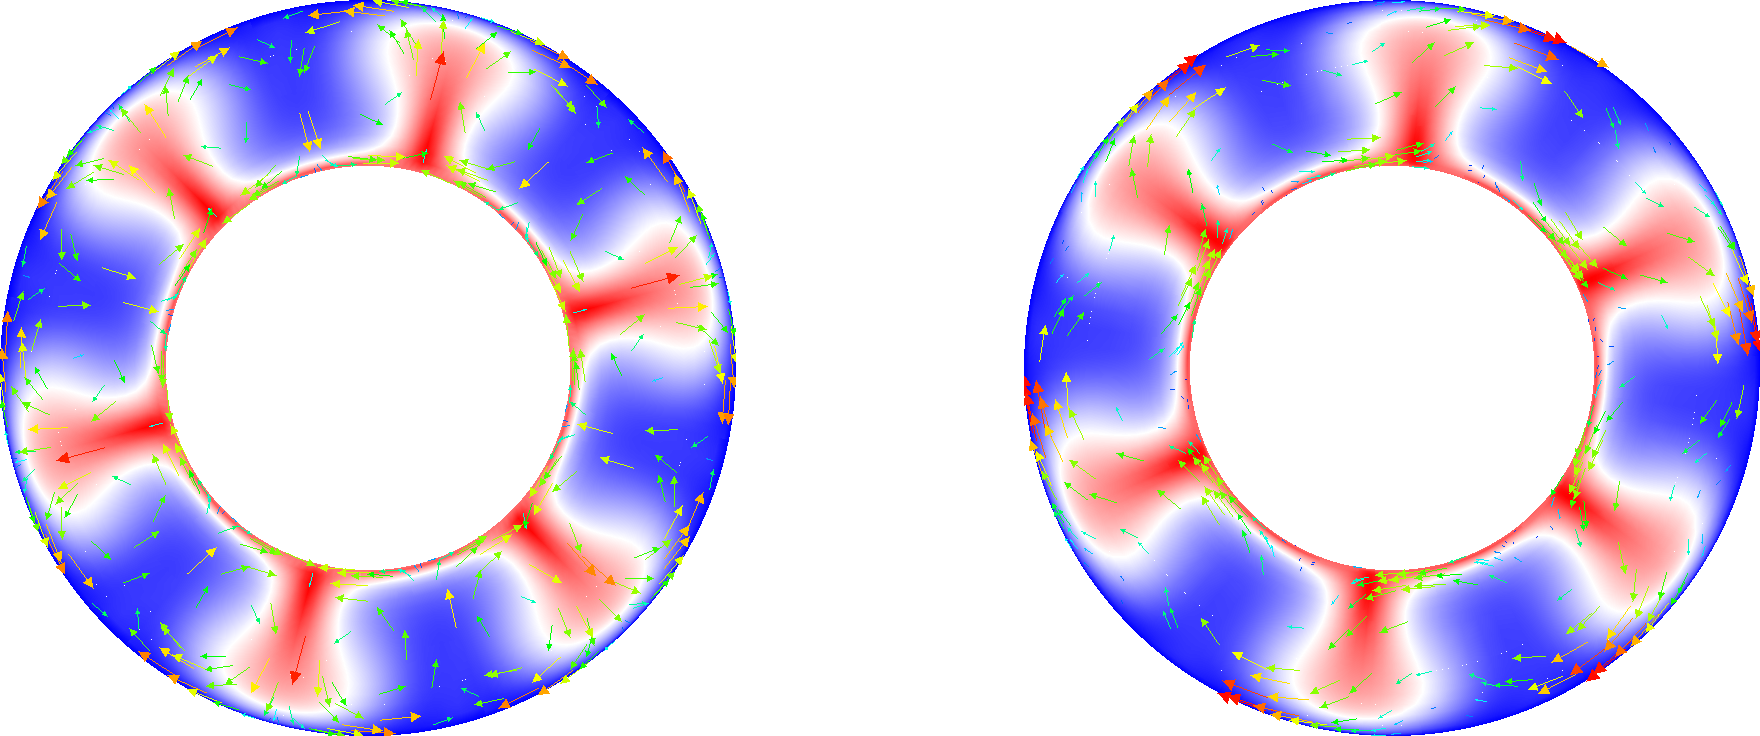
\includegraphics[width=0.8\textwidth]{rigid_rotation.png}
  \caption{\it Example of nullspace removal.
On the left the nullspace (a rigid rotation) is removed, and the velocity vectors accurately
show the mantle flow. On the right there is a significant clockwise rotation to the velocity
solution which is making the more interesting flow features difficult to see. }
  \label{fig:rigid_rotation}
\end{figure}


\subsection{Particles}
\label{sec:particles}

\aspect{} can, optionally, also deal with particles (sometimes called
``tracers''). Particles can be thought of as point-like objects that are simply
advected along with the flow. In other words, if $\mathbf u(\mathbf x,t)$ is the
flow field that results from solving equations
\eqref{eq:stokes-1}--\eqref{eq:stokes-2}, then the $k$th particle's position
satisfies the equations
\begin{align}
  \frac{d}{dt} \mathbf x_k(t)
  = \mathbf u(\mathbf x_k(t),t).
\end{align}
The initial positions of all particles also need to be given and are usually
either chosen randomly, based on a fixed pattern, or are read from a file.

Particles are typically used to track visually where material that starts
somewhere ends up after some time of a simulation. It can also be used to track
the \textit{history} of the volume of the fluid that surrounds a particle, for
example by tracking how much strain has accumulated, or what the minimal or maximal
temperature may have been in the medium along the trajectory of a particle. To
this end, particles can carry \textit{properties}. These are scalar-
or vector-valued quantities that are attached to each particle, that are
initialized at the beginning of a simulation, and that are then updated at each time step. In other words, if we
denote by $\mathbf p_{k,m}(t)$ the value of the $m$th property attached to
the $k$th particle, then $\mathbf p_{k,m}(t)$ will satisfy a differential
equation of the form
\begin{align*}
  \frac{\partial}{\partial t} \mathbf p_{k,m}(t)
  = \mathbf g_m\left(\mathbf p_{k,m},
  p(\mathbf x_k(t),t)), T(\mathbf x_k(t),t)),
  \varepsilon(\mathbf u(\mathbf x_k(t),t)),
  \mathfrak c(\mathbf x_k(t),t)\right).
\end{align*}
The exact form of $\mathbf g_m$ of course depends on what exactly a particular
property represents. Like with compositional fields (see
Section~\ref{sec:compositional}), it is possible to describe the right hand side
$\mathbf g_m$ in ways that also allows for impulse (delta) functions in time.

How particles are used in practice is probably best explained using examples. To
this end, see in particular Section~\ref{sec:cookbooks-particles}. All
particle-related input parameters are listed in
Section~\ref{parameters:Postprocess/Particles}. The implementation of particles is
discussed in great detail in \cite{gassmoeller_particles}.



\subsection{Geometric Multigrid}
\label{sec:gmg}

\aspect{} can optionally use a Geometric Multigrid Solver (GMG) for the efficient solution
of the Stokes system (velocity and pressure). When used correctly, this can
reduce the compute time spent in the solver by about a factor of 3,
and decrease the memory requirements by a factor of 10.
For more details
about the method see~\cite{clevenger_stokes19,clevenger_par_gmg}.

To take advantage of the GMG solver, you need to:
\begin{enumerate}
 \item Enable it in your parameter file, namely:
\lstinputlisting[language=prmfile]{cookbooks/overview/doc/gmg-enable.part.prm.out}
  See~\ref{parameters:Solver_20parameters/Stokes_20solver_20parameters} for other
  parameters that influence the solver behavior.

\item
  \index[prmindex]{Material averaging}
  \index[prmindexfull]{Material model!Material averaging}
  The GMG solver requires that the viscosity is averaged, either as a constant (for example by using harmonic averaging)
  or as a $Q_1$ averaging. (See Section~\ref{sec:sinker-with-averaging}
  for more about averaging.) Averaging other properties is optional. You can
  use
\lstinputlisting[language=prmfile]{cookbooks/overview/doc/gmg-average.part.prm.out}
for example. Note that $Q_1$ averaging is a bit slower than averaging to a constant per cell, but it
might provide more accurate solutions.

\item Run in release mode. The GMG solver depends on running optimized code, so using optimized mode
is more important than for other parts of ASPECT to get good
performance. (Of course, the GMG solver also runs in debug mode, and
you should do so while setting up a model. You will just not get the
same speedup from the non-GMG to the GMG solver in debug mode as you
get in release mode.)

\item Enable vectorization optimizations. The GMG solver takes advantage of special instructions (AVX2, AVX512)
in modern CPUs and requires these do be enabled when compiling \dealii{}. This can be achieved by passing the
compiler flag \texttt{CMAKE\_CXX\_FLAGS='-march=native'} to CMake or setting \texttt{NATIVE\_OPTIMIZATIONS=true} in \texttt{candi.cfg} when using candi (see~\ref{sec:installation} for more information).
When you have vectorization enabled, ASPECT will report something like
this:
\begin{lstlisting}[frame=single,language=ksh]
-----------------------------------------------------------------------------
-- This is ASPECT, the Advanced Solver for Problems in Earth's ConvecTion.
--     . version 2.3.0-pre
--     . using deal.II 9.2.0
--     .       with 64 bit indices and vectorization level 3 (512 bits)
--     . using Trilinos 12.10.1
--     . using p4est 2.2.0
--     . running in OPTIMIZED mode
--     . running with 114688 MPI processes
-----------------------------------------------------------------------------

Vectorization over 8 doubles = 512 bits (AVX512), VECTORIZATION_LEVEL=3
\end{lstlisting}
Without optimizations enabled, the output will be ``and vectorization
level 1 (128 bits)'' in the fourth line above.
\end{enumerate}




\section{Installation}
\label{sec:installation}

There are three distinct ways to install ASPECT -- compilation
from source, installing a virtual machine, and using a Docker container --
each providing distinct advantages and disadvantages. In this section we
describe all three options and start with a summary of their properties to
guide users to an informed decision about the best option for their purpose.

\begin{table}[htb]
  \center
  \begin{tabular}{|c|ccc|}
    \hline
    Feature & Compile \& Install & Virtual Machine & Docker Container \\
    \hline
    Speed overhead          & 0\%   & 30\%     & 0--5\%    \\
    Disk overhead           & 0~GB  & 1~GB     & 200~MB       \\
    Knowledge required      & Much  & Very Little & Little    \\
    Root privileges required & No   & No (installed VM software) & Partially  \\
    Embedded in native environment & Yes & No  & Partially    \\
    MacOS support           & Yes   & Yes      & Yes    \\
    Windows support         & No    & Yes      & Yes    \\
    Local parallelization   & Yes   & Yes      & Yes            \\
    Massively parallel computations & Yes & No & No \\
    Modifying ASPECT        & Possible & Possible & Possible \\
    Configuring dependencies & Possible & No   & No \\ \hline
  \end{tabular}
  \caption{\it Features of the different installation options of \aspect{}.}
  \label{tab:install-options}
\end{table}

The available options can be best presented in form of typical use cases:

\begin{enumerate}
\item Virtual Machine (\aspect{} beginner and tutorial participant): The
virtual machine image provides a fully prepared user environment that contains
installations of \aspect{}, all required libraries, and visualization software
on top of a full Linux environment. This way beginning users and tutorial
participants can work in a unified  environment, thus minimizing installation
time and technical problems. Due to the overhead of virtualizing a full
operating system this installation typically needs more space, and is
approximately 30~\% slower than a native installation. Additionally working in a
virtual machine `feels' differently from working in your usual desktop
environment. The virtual machine can be run on all host operating systems that
can run a virtualization software like VirtualBox (e.g. Linux, Apple MacOS,
Microsoft Windows).

\item Docker Container (advanced user with no need to configure/change the
underlying libraries, possibly changing parts of \aspect): Docker containers are
lightweight packages that only encapsulate the minimal dependencies to run an
application like \aspect{} on top of the host operating system. They allow easy
installation and usage of \aspect{} in a unified environment, while relying on
the user's operating system to provide visualization software and model input
data. When compared to the virtual machine it is simple to exchange files
between the host operating system and the docker container, and it provides the
benefit to work in the desktop environment you are used to. They have very
little overhead in terms of memory and speed compared to virtual machines, and
allow for reproducible computations. The container is set up with a standard
\aspect{} installation, but this can be modified by advanced users (source code
development within the container is possible).

\item Compile \& Install (advanced users and developers with the need to
reconfigure underlying libraries or running massively parallel models): The most
advanced option is to compile and install \aspect{} from source. This allows
maximal control over the underlying libraries like \trilinos{} and \dealii{}, as
well as easy modifications to \aspect{} by recompiling a modified source
directory. Our installation instructions cover most Linux and MacOS operating
systems, but incompatibilities on individual systems can always occur and make
the installation more cumbersome. If you are planning to run massively parallel
computations on a compute cluster this is likely your only option. Since
clusters usually have a very individual setup, it is always a good idea to ask
IT support staff for help when installing \aspect{}, to avoid hard to reproduce
setup problems, and performance penalties.
\end{enumerate}

\subsection{Docker Container}
\label{subsec:docker_container}

\subsubsection{Installing Docker and downloading the \aspect{} image}

Docker is a lightweight virtualization software that allows to ship
applications with all their dependencies in a simple way. It is outside of the
scope of this manual to explain all possible applications of Docker, and we
refer to the introduction (\url{https://www.docker.com/what-docker}) and
installation and quickstart guides
(\url{https://www.docker.com/products/docker}) on the Docker website for more
detailed descriptions of how to set up and use the docker engine. More
importantly Docker provides a marketplace for exchanging prepared docker images
(called Docker Hub). After setting up the docker engine downloading a
precompiled \aspect{} image from Docker Hub is as simple as typing in a
terminal:

\begin{lstlisting}[frame=single,language=ksh]
docker pull geodynamics/aspect
\end{lstlisting}

Note that the transfer size of the compressed image containing \aspect{} and
all its dependencies is about 900~MB. When extracted the image requires about
3.2~GB of disk space.

\subsubsection{Running \aspect{} models}
Although it is possible to use the downloaded \aspect{} docker image in a
number of different ways, we recommend the following workflow:

\begin{enumerate}
\item Create your \aspect{} input file in a folder of your choice (possibly
also containing any input data that is required by your model) and navigate in a
terminal into that directory.
\item Run the docker image and mount the current directory as a read-only
volume into the docker container\footnote{Note that it is possible to mount a
directory as writeable into the container. However, this is often associated
with file permission conflicts between the host system and the container.
Therefore, we recommend this slightly more cumbersome, but also more reliable
workflow.}. This is accomplished by specifying the -v flag followed by
the absolute path on the host machine, colon, absolute path within the docker
container, colon, and specifying read-only permissions as in the example below.

Make sure your parameter file specifies a model output directory \textit{other}
than the input directory, e.g. \texttt{/home/dealii/aspect/model\_output}. When
you have started the container run the aspect model inside the container. Note
that there are two \aspect{} executables in the work directory of the container:
\texttt{aspect} and \texttt{aspect-release}. For a discussion of the
different versions see Section~\ref{sec:debug-mode}, in essence: You should run
\texttt{aspect} first to check your model for errors, then run
\texttt{aspect-release} for a faster model run.

To sum up, the steps you will want to execute are:
\begin{lstlisting}[frame=single,language=ksh,showstringspaces=false]
docker run -it -v "$(pwd):/home/dealii/aspect/model_input:ro" \
  geodynamics/aspect:latest bash
\end{lstlisting}

Within the container, simply run your model by executing:

\begin{lstlisting}[frame=single,language=ksh]
./aspect model_input/your_input_file.prm
\end{lstlisting}

\item After the model has finished (or during the model run if you want to check
intermediate results) copy the model output out of the container into your
current directory. For this you need to find the name or ID of the docker
container by running \texttt{docker ps -a} in a separate terminal first. Look
for the most recently started container to identify your current \aspect{}
container.

Commands that copy the model output to the current directory could be:
\begin{lstlisting}[frame=single,language=ksh]
docker ps -a # Find the name of the running / recently closed container in the output
docker cp CONTAINER_NAME:/home/dealii/aspect/model_output .
\end{lstlisting}

\item The output data is saved inside your container even after the computation
finishes and even when you stop the container. After you have copied the data
out of the container you should therefore delete the container to avoid
duplication of output data. Even after deleting you will always be able to start
a new container from the downloaded image following step 2. Deleting the
finished container can be achieved by the \texttt{docker container prune}
command that removes any container that is not longer running.
\note{If you own other finished containers that you want to keep use
\texttt{docker container rm CONTAINER\_NAME} to only remove the container named
\texttt{CONTAINER\_NAME}.}

To remove all finished containers use the following command:
\begin{lstlisting}[frame=single,language=ksh]
docker container prune
\end{lstlisting}
Alternatively only remove a particular container:
\begin{lstlisting}[frame=single,language=ksh]
docker container rm CONTAINER_NAME
\end{lstlisting}
\end{enumerate}

You are all set. Repeat steps 1-4 of this process as necessary when updating
your model parameters.

\subsubsection{Developing \aspect{} within a container}

The above given workflow does not include advice on how to modify \aspect{}
inside the container. We recommend a slightly different workflow for advanced
users that want to modify parts of \aspect{}. The \aspect{} docker container
itself is build on top of a \dealii{} container that contains all dependencies
for compiling \aspect{}. Therefore it is possible to run the deal.II container,
mount an \aspect{} source directory from your host system and compile it inside
of the container. An example workflow could look as following (assuming you
navigated in a terminal into the modified \aspect{} source folder):

\begin{lstlisting}[frame=single,language=ksh,showstringspaces=false]
docker pull geodynamics/aspect:latest
docker run -it -v "$(pwd):/home/dealii/aspect:ro" geodynamics/aspect:latest
\end{lstlisting}

Inside of the container you now find a read-only \aspect{} directory that
contains your modified source code. You can compile and run a model inside the
container, e.g. in the following way:

\begin{lstlisting}[frame=single,language=ksh]
mkdir aspect-build
cd aspect-build
cmake -DCMAKE_BUILD_TYPE=Debug $HOME/aspect
make -j4
./aspect $HOME/aspect/cookbooks/shell_simple_2d/shell_simple_2d.prm
\end{lstlisting}

To avoid repeated recompilations of the \aspect{} source folder we recommend to
reuse the so prepared container instead of starting new containers based on the
\dealii{} image. This can be achieved by the following commands outside of the
container:

\begin{lstlisting}[frame=single,language=ksh]
docker ps -a # Find the name of the running / recently closed container in the output
docker restart CONTAINER_NAME
docker attach CONTAINER_NAME
\end{lstlisting}

For more information on the differences between using images and containers,
and how to attach additional terminals to a running container, we refer to the
docker documentation (e.g.
\url{https://docs.docker.com/engine/getstarted/step_two/}).

\subsection{Virtual Machine}

\subsubsection{Installing VM software and setting up the virtual machine}

The \aspect{} project provides an experimental virtual machine containing a
fully configured version of \aspect{}. To use this machine, you will need to
install VirtualBox (\url{http://www.virtualbox.org/}) on your machine, and then
import a virtual machine image that can be downloaded from
\url{http://www.math.clemson.edu/~heister/dealvm/}. Note, however, that the
machine image is several gigabytes in size and downloading will take a while.
After downloading and installing the virtual image it is convenient to set up a
shared folder between your host system and the virtual machine to exchange model
files and outputs.

\subsubsection{Running \aspect{} models}

The internal setup of the virtual machine is similar to the Docker container
discussed above, except that it contains a full-featured desktop environment.
Also note that the user name is \texttt{ubuntu}, not \texttt{dealii} as in the
Docker container. Again there are multiple ways to use the virtual machine, but
we recommend the following workflow:

\begin{enumerate}
\item Create your \aspect{} input file in the shared folder and start the
virtual machine.
\item Navigate in a terminal to your model directory.
\item Run your model using the provided \aspect{} executable:

\begin{lstlisting}[frame=single,language=ksh]
~/aspect/aspect your_input_file.prm
\end{lstlisting}

\item The model output should automatically appear on your host machine in the
shared directory.

\item After you have verified that your model setup is correct, you might want
to consider recompiling \aspect{} in release mode to increase the speed of the
computation. See Section~\ref{sec:debug-mode} for a discussion of debug and
release mode.

\item Visualize your model output either inside of the virtual machine
(ParaView and VisIt are pre-installed), or outside on your host system.
\end{enumerate}

You are all set. Repeat steps 1-6 of this process as necessary when updating
your model parameters.

\subsection{Local installation}

This is a brief explanation of how to compile and install the required dependencies and
\aspect{} itself. This installation procedure guarantees fastest runtimes, and largest flexibility,
but usually requires more work than the options mentioned in the previous sections.
While it is possible to install ASPECT's dependencies in particular \pfrst{}, \trilinos{},
and \dealii{} manually, we recommend to use the
\texttt{candi} software (see \url{https://github.com/dealii/candi}). \texttt{candi} was written
as an installation program for deal.II, and includes a number of system specific instructions
that will be listed when starting the program. It can be flexibly configured to allow for
non-default compilers or libraries (e.g. Intel's MKL instead of LAPACK) by changing entries
in the configuration file \texttt{candi.cfg}, or by providing platform specific installation files.

In case you encounter problems during the installation, please consult our wiki
(\url{https://github.com/geodynamics/aspect/wiki}) for frequently asked
questions and special instructions for MacOS users, before posting your
questions on the forum (\url{https://community.geodynamics.org/c/aspect}).

\subsubsection{System prerequisites}

\texttt{candi} will show system specific instructions on startup, but its prerequisites
are relatively widely used and packaged
for most operating systems. You will need compilers for C, C++ and
Fortran, the GNU make system, the CMake build system, and the libraries and
header files of BLAS, LAPACK and zlib, which is used for compressing
the output data. To use more than one process for your computations
you will need to install a MPI library, its headers and the
necessary executables to run MPI programs. There are some optional packages
for additional features, like the HDF5 libraries for additional output formats
 and Numdiff for checking \aspect{}'s test
results with reasonable accuracy, but these are not strictly required, and in
some operating systems they are not available as packages but need to be
compiled from scratch.
Finally, for obtaining a recent development version of \aspect{} you will
need the git version control system.

An exemplary command to obtain all required packages on Ubuntu 14.04 would be:
\begin{verbatim}
sudo apt-get install build-essential \
                     cmake \
                     gcc \
                     g++ \
                     gfortran \
                     git \
                     libblas-dev \
                     liblapack-dev \
                     libopenmpi-dev \
                     numdiff \
                     openmpi-bin \
                     zlib1g-dev
\end{verbatim}

\subsubsection{Using candi to compile dependencies}

In its default configuration \texttt{candi} downloads and
compiles a \dealii{} configuration that is able to run \aspect, but it
also contains a number of packages that are not required (and that can
be safely disabled if problems occur during the
installation). We require at least the packages \pfrst{}, \trilinos{},
and finally \dealii{}.

At the time of this writing \texttt{candi} will install \pfrst{} 2.2,
\trilinos{} 12.18.1, and \dealii{} 9.3.0.
We strive to keep the development version of \aspect{} compatible with
the latest release of \dealii{} and the current \dealii{} development
version at any time, and we usually support several older versions of
\pfrst{} and \trilinos{}.

\begin{enumerate}
\item \textit{Obtaining candi:} Download \texttt{candi} by running
    \begin{verbatim}
    git clone https://github.com/dealii/candi
    \end{verbatim}
    in a directory of your choice.

\item \textit{Installing \dealii{} and its dependencies:} Execute \texttt {candi} by running
    \begin{verbatim}
    cd candi
    ./candi.sh -p INSTALL_PATH
    \end{verbatim}
    (here we assume you replace \texttt{INSTALL\_PATH} by the path were
    you want to install all dependencies and \dealii{}, typically a directory inside
    \texttt{\$HOME/bin} or a similar place).
    This step might take a long time, but can be parallelized by adding
    \texttt{-jN}, where
    \texttt{N} is the number of CPU cores available on your computer. Further configuration options
    and parameters are listed at \url{https://github.com/dealii/candi}. In case you encounter
    problems during this step, please read the error message, and consult our wiki
    (\url{https://github.com/geodynamics/aspect/wiki}) for common installation problems,
    before asking on the forum (\url{https://community.geodynamics.org/c/aspect}).

\item You may now want to configure your environment to make it aware of the newly installed
    packages. This can be achieved by adding the line
    \texttt{source INSTALL\_PATH/configuration/enable.sh} to the file responsible for setting
    up your shell environment\footnote{For bash this would be the file \texttt{\~{}/.bashrc}.}
    (again we assume you replace \texttt{INSTALL\_PATH} by the patch chosen in the previous step).
    Then close the terminal and open it again to activate the change.

\item \textit{Testing your installation:} Test that your installation works
  by compiling the {\texttt{step-32}} example that you can find in
  {\texttt{\$DEAL\_II\_DIR/examples/step-32}}. Prepare and compile by running {\texttt{cmake . \&\& make}}
  and run with {\texttt{mpirun -n 2 ./step-32}}.

\end{enumerate}

Congratulations, you are now set up for compiling \aspect{} itself.

\subsubsection{Obtaining \aspect{} and initial configuration}

The development version of \aspect{} can be downloaded by executing the command
\begin{verbatim}
 git clone https://github.com/geodynamics/aspect.git
\end{verbatim}
If {\texttt{\$DEAL\_II\_DIR}} points to your \dealii{} installation, you can configure
\aspect{} by running
\begin{verbatim}
 mkdir build; cd build; cmake ..
\end{verbatim}
in the \aspect{} directory created by the {\texttt{git clone}} command above.
If you did not set {\texttt{\$DEAL\_II\_DIR}} you have to supply cmake with the location:
\begin{verbatim}
 cmake -DDEAL_II_DIR=/u/username/deal-installed/ ..
\end{verbatim}

This will create an ``out-of-source`` build, where the build directory is
different from the source directory. While in-source builds (where you run
\texttt{cmake .} in your source directory), are supported, we strongly
recommend an out-of-source build as described above. Specifically, running
the whole test suite (see Section~\ref{sec:running_tests}) is only supported
this way.

\subsubsection{Compiling \aspect{} and generating documentation}
\label{sec:compiling}

After downloading \aspect{} and having built the libraries it builds on, you
can compile it by typing
\begin{verbatim}
  make
\end{verbatim}
on the command line (or \texttt{make -jN} if you have multiple processors in
your machine, where \texttt{N} is the number of processors). This builds the
\aspect{} executable which will reside in the \texttt{build} directory
and will be named \texttt{aspect}. To run \aspect{} from the main source directory
you would need to reference it as \texttt{./build/aspect}.
If you intend to
modify \aspect{} for your own experiments, you may want to also generate
documentation about the source code. This can be done using the command
\begin{verbatim}
  cd doc; make
\end{verbatim}
which assumes that you have the \texttt{doxygen} documentation generation tool
installed. Most Linux distributions have packages for \texttt{doxygen}. The
result will be the file \url{doc/doxygen/index.html} that is the starting
point for exploring the documentation.


%%%%%%%%%%%%%%%%%%%%%%

\section{Running \aspect}
\label{sec:running}

\subsection{First steps}
\label{sec:first-steps}
Before trying to set up a model to answer your particular research questions,
we advise you to get familiar with \aspect{} and its functionalities by
following these steps:
\begin{enumerate}
\item Watch the CIG \aspect{} tutorials (\url{https://www.youtube.com/playlist?list=PLdy04DoEepEyeS_HZwa0Ws0kW5Rs2wsQ6})
that will show you how to run \aspect{} and construct new setups yourself.
\item Go through the cookbooks in this manual, see Section~\ref{sec:cookbooks}.
\item Go through the benchmarks in this manual, see Section~\ref{sec:cookbooks-benchmarks}.
\item If you want to use some existing functionality that is not discussed in these resources,
search in the extensive tests directory. For example, to search for an initial temperature condition called
``spherical gaussian perturbation'' while in the \aspect{} directory, type:
\begin{verbatim}
  grep 'spherical gaussian perturbation' tests/*.prm
\end{verbatim}
This command will show you all the test input files that use this initial temperature condition.
You can also look up any of the parameters used in the input files in this manual.
\item Have a look at the \aspect{} GitHub repository. Here you can see the planned developments
(\url{https://github.com/geodynamics/aspect/projects/2}), current issues that others have reported
(\url{https://github.com/geodynamics/aspect/issues}), and what is currently being worked on
(\url{https://github.com/geodynamics/aspect/pulls}).
\item Have a look at our discussion forum when your model behaves unexpectedly
or you need functionality that does not exist yet. The \aspect{} community can tell you
whether they experienced something similar or are already working on the topic.
\item If you experience unexpected behavior that you expect is a bug and this problem
has not been reported as an issue on GitHub, please create a new issue so that everybody
is aware of the potential problem and can think of a fix. When creating a new issue,
it is very useful if you can provide a minimum working example, i.e. a small test setup
that demonstrates the issue and does not require modifications to the code. You can for example
modify one of the existing test input files, which typically take less than a minute to
run using only a few cores.
The test input file and an image illustrating the problem can be attached to the issue.
\end{enumerate}

\subsection{Overview}
\label{sec:running-overview}

After compiling \aspect{} as described above, you should have an executable
file in the build directory. It can be called in the build directory as follows:
\begin{verbatim}
  ./aspect parameter-file.prm
\end{verbatim}
or, if you want to run the program in parallel, using something like
\begin{verbatim}
  mpirun -np 4 ./aspect parameter-file.prm
\end{verbatim}
to run with 4 processors. In either case, the argument denotes the (path and)
name of a file that contains input parameters.%
\footnote{As a special case, if you call \aspect{} with an argument that
consists of two dashes, ``\texttt{-{}-}'', then the arguments will be read from
the standard input stream of the program. In other words, you could type the
input parameters into your shell window in this case (though that would be
cumbersome, \aspect{} would seem to hang until you finish typing all of your
input into the window and then terminating the input stream by typing
\texttt{Ctrl-D}). A more common case would be to use Unix pipes so that the
default
input of \aspect{} is the output of another program, as in a command like
\texttt{cat parameter-file.prm.in | mypreprocessor | ./aspect -{}-}, where
\texttt{mypreprocessor} would be a program of your choice that somehow
transforms the file \texttt{parameter-file.prm.in} into a valid input file,
for example to systematically vary one of the input parameters.

If you want to run \aspect{} in parallel, you can do something like
\texttt{cat parameter-file.prm.in | mypreprocessor | mpirun -np 4 ./aspect
  -{}-}. In cases like this, \texttt{mpirun} only forwards the output of
\texttt{mypreprocessor} to the first of the four MPI processes, which then
sends the text to all other processors.}
When you download \aspect{}, there are a number of sample input files in the
\texttt{cookbooks} directory, corresponding to the examples discussed in
Section~\ref{sec:cookbooks}, and input files for some of the benchmarks discussed
in Section~\ref{sec:cookbooks-benchmarks} are located in the \texttt{benchmarks}
directory. A full description of all parameters one can specify in these files
is given in Section~\ref{sec:parameters}.

Running \aspect{} with an input file
\footnote{For example by running \texttt{./aspect ../cookbooks/convection-box/convection-box.prm} in
your build directory.}
will produce output that will look
something like this (numbers will all be different, of course):
\begin{lstlisting}[frame=single,language=ksh]
-----------------------------------------------------------------------------
-- This is ASPECT, the Advanced Solver for Problems in Earth's ConvecTion.
--     . version 2.0.0-pre (include_dealii_version, c20eba0)
--     . using deal.II 9.0.0-pre (master, 952baa0)
--     . using Trilinos 12.10.1
--     . using p4est 2.0.0
--     . running in DEBUG mode
--     . running with 1 MPI process
-----------------------------------------------------------------------------

Number of active cells: 1,536 (on 5 levels)
Number of degrees of freedom: 20,756 (12,738+1,649+6,369)

*** Timestep 0:  t=0 years

   Rebuilding Stokes preconditioner...
   Solving Stokes system... 30+3 iterations.
   Solving temperature system... 8 iterations.

Number of active cells: 2,379 (on 6 levels)
Number of degrees of freedom: 33,859 (20,786+2,680+10,393)

*** Timestep 0:  t=0 years

   Rebuilding Stokes preconditioner...
   Solving Stokes system... 30+4 iterations.
   Solving temperature system... 8 iterations.

   Postprocessing:
     Writing graphical output: output/solution/solution-00000
     RMS, max velocity:        0.0946 cm/year, 0.183 cm/year
     Temperature min/avg/max:  300 K, 3007 K, 6300 K
     Inner/outer heat fluxes:  1.076e+05 W, 1.967e+05 W

*** Timestep 1:  t=1.99135e+07 years

   Solving Stokes system... 30+3 iterations.
   Solving temperature system... 8 iterations.

   Postprocessing:
     Writing graphical output: output/solution/solution-00001
     RMS, max velocity:        0.104 cm/year, 0.217 cm/year
     Temperature min/avg/max:  300 K, 3008 K, 6300 K
     Inner/outer heat fluxes:  1.079e+05 W, 1.988e+05 W

*** Timestep 2:  t=3.98271e+07 years

   Solving Stokes system... 30+3 iterations.
   Solving temperature system... 8 iterations.

   Postprocessing:
     RMS, max velocity:       0.111 cm/year, 0.231 cm/year
     Temperature min/avg/max: 300 K, 3008 K, 6300 K
     Inner/outer heat fluxes: 1.083e+05 W, 2.01e+05 W

*** Timestep 3:  t=5.97406e+07 years

...
\end{lstlisting}

The output starts with a header that lists the used \aspect{}, \dealii{},
\trilinos{} and \pfrst{} versions as well as the mode you compiled \aspect{} in
(see \ref{sec:debug-mode}), and the number of parallel processes
used\footnote{If you used the \texttt{git} version control system to download
\aspect{} and/or \dealii{}, as in this example, you will also get the current
branch, and unique revision identifier for the current version. This is very
important if you modify either software between releases, or you use a
development version that is not an official release. Note that this revision
can not track changes you made to the software that are not part of a git
commit.}.  With this information we strive to make
\aspect{} models as reproducible as possible.

The following output depends on the model, and in this case was produced by
a parameter file that, among other settings, contained the following values
(we will discuss many such input files in Section~\ref{sec:cookbooks}:
\lstinputlisting[language=prmfile]{cookbooks/overview/doc/simple.prm.out}

In other words, these run-time parameters specify that we should start with a
geometry that represents a spherical shell (see
Sections~\ref{parameters:Geometry_20model} and
\ref{parameters:Geometry_20model/Spherical_20shell} for details). The coarsest
mesh is refined 4 times globally, i.e., every cell is refined into four
children (or eight, in 3d) 4 times. This yields the initial number of 1,536
cells on a mesh hierarchy that is 5 levels deep. We then solve the problem
there once and, based on the number of adaptive refinement steps at the
initial time set in the parameter file, use the solution so computed to refine
the mesh once adaptively (yielding 2,379 cells on 6 levels) on which we start
the computation over at time $t=0$.

Within each time step, the output indicates the number of iterations performed
by the linear solvers, and we generate a number of lines of output by the
postprocessors that were selected (see
\index[prmindex]{List of postprocessors}
\index[prmindexfull]{Postprocess!List of postprocessors}
Section~\ref{parameters:Postprocess}). Here, we have selected to run all
postprocessors that are currently implemented in \aspect{} which includes the
ones that evaluate properties of the velocity, temperature, and heat flux as
well as a postprocessor that generates graphical output for visualization.

While the screen output is useful to monitor the progress of a simulation,
its lack of a structured output makes it not useful for later plotting things
like the evolution of heat flux through the core-mantle boundary. To this end,
\aspect{} creates additional files in the output directory selected in the
input parameter file
\index[prmindex]{Output directory}
\index[prmindexfull]{Output directory}
(here, the \texttt{output/} directory relative to the
directory in which \aspect{} runs). In a simple case, this will look as
follows:
\begin{lstlisting}[frame=single,language=ksh]
aspect> ls -l output/
total 932
-rw-rw-r-- 1 bangerth bangerth  11134 Dec 11 10:08 depth_average.gnuplot
-rw-rw-r-- 1 bangerth bangerth  11294 Dec 11 10:08 log.txt
-rw-rw-r-- 1 bangerth bangerth     42 Dec 11 10:07 original.prm
-rw-rw-r-- 1 bangerth bangerth 326074 Dec 11 10:07 parameters.prm
-rw-rw-r-- 1 bangerth bangerth 577138 Dec 11 10:07 parameters.tex
drwxr-xr-x 2 bangerth bangerth   4096 Dec 11 10:08 solution
-rw-rw-r-- 1 bangerth bangerth    484 Dec 11 10:08 solution.pvd
-rw-rw-r-- 1 bangerth bangerth    451 Dec 11 10:08 solution.visit
-rw-rw-r-- 1 bangerth bangerth   8267 Dec 11 10:08 statistics
\end{lstlisting}
The purpose of these files is as follows:
\begin{itemize}

\item \textit{Screen output:} The file \texttt{output/log.txt} contains a copy
  of the output that is printed to the terminal when you run \aspect{}.

\item \textit{A listing of all run-time parameters:} The file
  \texttt{output/original.prm} is a copy of the parameter file that was used
  in this computation. It is often useful to save this file together with
  simulation data to allow for the easy reproduction of computations later on.

  The \texttt{output/parameters.prm} file contains a complete listing of all
  run-time parameters. In particular, this includes the ones that have been
  specified in the input parameter file passed on the command line, but it
  also includes those parameters for which defaults have been used. This file
  can also be used to explore all available parameters and possible options as
  it contains the documentation of all parameters.

  Finally, there is \texttt{output/parameters.tex}, that lists the parameters
  like \texttt{output/parameters.prm} in \LaTeX{} format, and
  \texttt{output/parameters.json} in JSON format.

  While \texttt{output/parameters.prm} contains all parameters (with their
  default values if they were not specified), all formatting and comments are
  lost. As \texttt{output/original.prm} is identical to the prm you started
  \aspect{} with, it preserves comments and formatting while not outputting
  the default values (or documentation).

\item \textit{Graphical output files:} One of the postprocessors chosen
  in the parameter file used for this computation is the one that generates
  output files that represent the solution at certain time steps. The screen output
  indicates that it has run at time step 0, producing output files that start
  with \texttt{output/solution/solution-00000}. Depending on the settings in the
  parameter file, output will be generated every so many seconds or years of
  simulation time, and subsequent output files will then start with
  \texttt{output/solution/solution-00001}, all placed in the
  \texttt{output/solution} subdirectory. This is because there are often
  \textit{a lot} of output files: For many time steps, times the number of
  processors, so they are placed in a subdirectory so as not to make it more
  difficult than necessary to find the other files.

  At the current time, the
  default is that \aspect{} generates this output in VTK format%
  \footnote{The output is in fact in the VTU version of the VTK file
    format. This is the XML-based version of this file format in which
    contents are compressed. Given that typical file sizes for 3d simulation
    are substantial, the compression saves a significant amount of disk
    space.}  as that is widely used by a number of excellent visualization
  packages and also supports parallel visualization.%
  \footnote{The underlying \dealii{} package actually supports output in
    around a dozen different formats, but most of them are not very useful for
    large-scale, 3d, parallel simulations. If you need a different format than
    VTK, you can select this using the run-time parameters discussed in
    Section~\ref{parameters:Postprocess/Visualization}.}  If
  the program has been run with multiple MPI processes, then the list of
  output files will be \texttt{output/solution/solution-XXXXX.YYYY}
  denoting that this the \texttt{XXXXX}th time we create output files and that
  the file was generated by the \texttt{YYYY}th processor.

  VTK files can be visualized by many of the large visualization packages. In
  particular, the
  \href{https://visit.llnl.gov}{Visit} and
  \href{http://www.paraview.org/}{ParaView} programs, both
  widely used, can read the files so created. However, while VTK has become a
  de-facto standard for data visualization in scientific computing, there
  doesn't appear to be an agreed upon way to describe which files jointly make
  up for the simulation data of a single time step (i.e., all files with the
  same \texttt{XXXXX} but different \texttt{YYYY} in the example above). Visit
  and ParaView both have their method of doing things, through \texttt{.pvtu} and
  \texttt{.visit} files. To make it easy for you to view data, \aspect{}
  simply creates both kinds of files in each time step in which graphical data
  is produced, and these are then also placed into the subdirectories as
  \texttt{output/solution/solution-XXXXX.pvtu} and
  \texttt{output/solution/solution-XXXXX.visit}.

  The final two files of this kind, \texttt{output/solution.pvd} and
  \texttt{output/solution.visit}, are files that
  describes to ParaView and Visit, respectively, which
  \texttt{output/solution/solution-XXXXX.pvtu} and
  \texttt{output/solution/solution-XXXXX.YYYY.vtu} jointly form a complete
  simulation.
  In the former case, the file lists the \texttt{.pvtu} files of all
  timesteps together with the simulation time to which they correspond. In the
  latter case, it actually lists all \texttt{.vtu} that belong to one
  simulation, grouped by the timestep they correspond to.
  To visualize an entire simulation, not just a single time step, it is
  therefore simplest to just load one of these files, depending on whether you
  use ParaView or Visit.%
  \footnote{At the time of writing this, current versions of Visit (starting
    with version 2.5.1) actually have a bug that prevents them from
    successfully reading the \texttt{output/solution.visit} or
    \texttt{output/solution/solution-XXXXX.visit} files -- Visit believes that
    each of these files corresponds to an individual time step, rather than that a whole
    group of files together form one time step. This bug is not fixed in Visit
    2.6.3, but may be fixed in later versions.}
  Because loading an \textit{entire} simulation is the most common use case,
  these are the two files you will most often load, and so they are placed in
  the \texttt{output} directory, not the subdirectory where the actual
  \texttt{.vtu} data files are located.

  For more on visualization, see also Section~\ref{sec:viz}.

\item \textit{A statistics file:} The \texttt{output/statistics} file contains
  statistics collected during each time step, both from within the simulator
  (e.g., the current time for a time step, the time step length, etc.) as well
  as from the postprocessors that run at the end of each time step. The file
  is essentially a table that allows for the simple production of time
  trends. In the example above, and at the time when we are writing this
  section, it looks like this:
  \begin{lstlisting}[frame=single,language=ksh,showstringspaces=false]
# 1: Time step number
# 2: Time (years)
# 3: Iterations for Stokes solver
# 4: Time step size (year)
# 5: Iterations for temperature solver
# 6: Visualization file name
# 7: RMS velocity (m/year)
# 8: Max. velocity (m/year)
# 9: Minimal temperature (K)
# 10: Average temperature (K)
# 11: Maximal temperature (K)
# 12: Average nondimensional temperature (K)
# 13: Core-mantle heat flux (W)
# 14: Surface heat flux (W)
0 0.000e+00 33 2.9543e+07 8                             "" 0.0000 0.0000 0.0000 0.0000    ...
0 0.000e+00 34 1.9914e+07 8 output/solution/solution-00000 0.0946 0.1829 300.00 3007.2519 ...
1 1.991e+07 33 1.9914e+07 8 output/solution/solution-00001 0.1040 0.2172 300.00 3007.8406 ...
2 3.982e+07 33 1.9914e+07 8                             "" 0.1114 0.2306 300.00 3008.3939 ...
  \end{lstlisting}
  The actual columns you have in your statistics file may differ from the ones above,
  but the format of this file should be obvious. Since the hash mark is a comment
  marker in many programs (for example, \texttt{gnuplot} ignores lines in text
  files that start with a hash mark), it is simple to plot these columns as time
  series. Alternatively, the data can be imported into a spreadsheet and
  plotted there.
\note{As noted in Section~\ref{sec:non-dimensional}, \aspect{} can be
  thought of as using the meter-kilogram-second (MKS, or SI) system. Unless otherwise noted,
  the quantities in the output file are therefore also in MKS units.}

  A simple way to plot the contents of this file is shown in Section~\ref{sec:viz-stat}.

\item \textit{Output files generated by other postprocessors:} Similar to the
  \texttt{output/statistics} file, several of the existing
  postprocessors one can select from the parameter file generate their
  data in their own files in the output directory. For example, \aspect{}'s
  ``depth average'' postprocessor will write depth-average statistics into
  the file \texttt{output/depth\_average.gnuplot}.
  Input parameters chosen in the input file control how often this file is
  updated by the postprocessor, as well as what graphical file format to use (if
  anything other than \texttt{gnuplot} is desired).

  By default, the data is written in text format that can be easily visualized,
  see for example Figure~\ref{fig:depthaverage}. The plot
  shows how an initially linear temperature profile forms upper and lower
  boundary layers.

\begin{figure}[tbp]
  \centering
  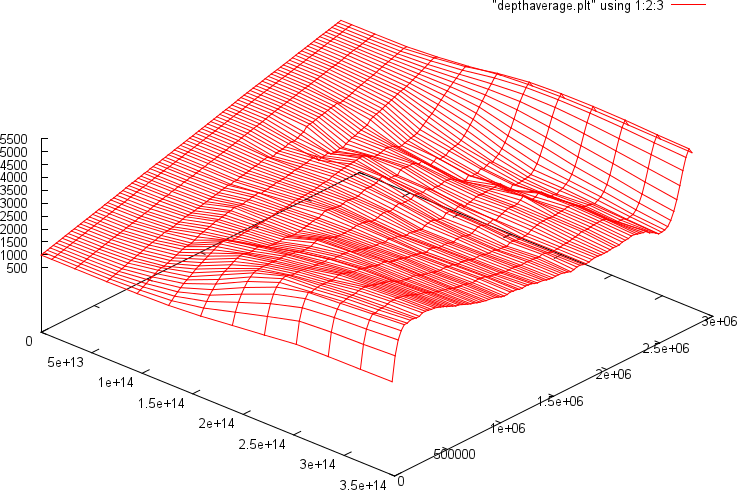
\includegraphics[width=0.6\textwidth]{depthaverage2.png}
  \caption{\it Example output for depth average statistics. On the left axis are 13 time
  steps, on the right is the depth (from the top at 0 to the bottom of the mantle on the
  far right), and the upwards pointing axis is the average temperature. This
  plot is generated by gnuplot, but the depth averages can be written in many
  other output formats as well, if preferred (see
  Section~\ref{parameters:Postprocess/Depth_20average}).}
  \label{fig:depthaverage}
\end{figure}

\end{itemize}

There are other parts of \aspect{} that may also create files in the output
directory. For example, if your simulation includes advecting along particles
(see Section~\ref{sec:particles}), then visualization information for these
particles will also appear in this file. See
Section~\ref{sec:cookbooks-particles} for an example of how this looks like.


\subsection{Selecting between 2d and 3d runs}
\label{sec:2d-vs-3d}

\aspect{} can solve both two- and three-dimensional problems.%
\footnote{For a description of what exactly we mean when we consider
two-dimensional models, see Section~\ref{sec:meaning-of-2d}.}
You select which one you want by putting a line like the following into
\index[prmindex]{Dimension}
\index[prmindexfull]{Dimension}
the parameter file (see Section~\ref{sec:parameters}):
\lstinputlisting[language=prmfile]{cookbooks/overview/doc/dim.part.prm.out}

Internally, dealing with the dimension builds on a feature in
\dealii{}, upon which \aspect{} is based, that is called
\textit{dimension-independent programming}. In essence, what this does is that
you write your code only once in a way so that the space dimension is a
variable (or, in fact, a template parameter) and you can compile the code for
either 2d or 3d. The advantage is that codes can be tested and debugged in 2d
where simulations are relatively cheap, and the same code can then be
re-compiled and executed in 3d where simulations would otherwise be
prohibitively expensive for finding bugs; it is also a useful feature when
scoping out whether certain parameter settings will have the desired effect by
testing them in 2d first, before running them in 3d. This feature is discussed
in detail in the
\href{https://www.dealii.org/developer/doxygen/deal.II/step_4.html}{\dealii{}
  tutorial program step-4}.
Like there, all the functions and classes in
\aspect{} are compiled for both 2d and 3d. Which dimension is actually
called internally depends on what you have set in the input file, but
in either case, the machine code generated for 2d and 3d results from
the same source code and should, thus, contain the same set of
features and bugs. Running in 2d and 3d should therefore yield
comparable results. Be prepared to wait much longer for
computations to finish in the latter case, however.


\subsection{Debug or optimized mode}
\label{sec:debug-mode}

\aspect{} utilizes a \dealii{} feature called \textit{debug
  mode}. By default, \aspect{} uses debug mode, i.e., it calls a version of
the \dealii{} library that contain lots of checks for the correctness of
function arguments, the consistency of the internal state of data structure,
etc. If you program with \dealii{}, for example to extend \aspect{}, it has
been our experience over the years that, by number, most programming errors are of the
kind where one forgets to initialize a vector, one accesses data that has not
been updated, one tries to write into a vector that has ghost elements,
etc. If not caught, the result of these bugs is that parts of the program use
invalid data (data written into ghost elements is not communicated to other
processors), that operations simply make no sense (adding vectors of different
length), that memory is corrupted (writing past the end of an array) or, in
rare and fortunate cases, that the program simply crashes.

Debug mode is designed to catch most of these errors: It enables some 7,300
assertions (as of late 2011) in \dealii{} where we check for errors like the
above and, if the condition is violated, abort the program with a detailed
message that shows the failed check, the location in the source code, and a
stacktrace how the program got there. The downside of debug mode is, of
course, that it makes the program much slower -- depending on application by a
factor of 4--10. An example of the speedup one can get is shown in
Section~\ref{sec:cookbooks-simple-box}.

\aspect{} by default uses debug mode because most users will want to play with
the source code, and because it is also a way to verify that the compilation
process worked correctly. If you have verified that the program runs correctly
with your input parameters, for example by letting it run for the first 10
time steps, then you can switch to optimized mode by compiling \aspect{}
with the command\footnote{Note that this procedure also changed with the switch to cmake.}
\begin{verbatim}
 make release
\end{verbatim}
and then compile using
\begin{verbatim}
 make
\end{verbatim}
To switch back to debug mode type:
\begin{verbatim}
 make debug
\end{verbatim}

\note{It goes without saying that if you make significant modifications to the
  program, you should do the first runs in debug mode to verify that your
  program still works as expected.}


\subsection{Visualizing results}
\label{sec:viz}

Among the postprocessors that can be selected in the input parameter file (see
Sections~\ref{sec:running-overview} and
\ref{parameters:Postprocess/Visualization}) are some that can produce files in
a format that can later be used to generate a graphical visualization of the
solution variables $\mathbf u, p$ and $T$ at select time steps, or of
quantities derived from these variables (for the latter, see
Section~\ref{sec:viz-postpostprocessors}).

By default, the files that are generated are in VTU format, i.e., the
XML-based, compressed format defined by the VTK library, see
\url{http://public.kitware.com/VTK/}. This file format has become a broadly
accepted pseudo-standard that many visualization program support, including
two of the visualization programs used most widely in computational science:
Visit (see \url{https://visit.llnl.gov/}) and ParaView (see
\url{http://www.paraview.org/}). The VTU format has a number of
advantages beyond being widely distributed:
\begin{itemize}
\item It allows for compression, keeping files relatively small even for
  sizable computations.
\item It is a structured XML format, allowing other programs to read it
  without too much trouble.
\item It has a degree of support for parallel computations where every
  processor would only write that part of the data to a file that this
  processor in fact owns, avoiding the need to communicate all data to a
  single processor that then generates a single file. This requires a master
  file for each time step that then contains a reference to the individual
  files that together make up the output of a single time step. Unfortunately,
  there doesn't appear to be a standard for these master records; however,
  both ParaView and Visit have defined a format that each of these programs
  understand and that requires placing a file with ending \texttt{.pvtu} or
  \texttt{.visit} into the same directory as the output files from each
  processor. Section~\ref{sec:running-overview} gives an example of what can
  be found in the output directory.
\end{itemize}

\note{You can select other formats for output than VTU, see the run-time
  parameters in Section~\ref{parameters:Postprocess/Visualization}. However,
  none of the numerous formats currently implemented in \dealii{} other than
  the VTK/VTU formats allows for splitting up data over multiple files in case
  of parallel computations, thus making subsequent visualization of the entire
  volume impossible. Furthermore, given the amount of data \aspect{} can
  produce, the compression that is part of the VTU format is an important part
  of keeping data manageable.
\index[prmindex]{Output format}
\index[prmindexfull]{Postprocess!Visualization!Output format}
}

\subsubsection{Visualization the graphical output using \textit{Visit}}
In the following, let us discuss the process of visualizing a 2d computation
using Visit. The steps necessary for other visualization programs will
obviously differ but are, in principle, similar.

To this end, let us consider a simulation of convection in a box-shaped, 2d
region (see the ``cookbooks'' section, Section~\ref{sec:cookbooks}, and in
particular Section~\ref{sec:cookbooks-simple-box} for
the input file for this particular model). We can run the program with 4 processors using
\begin{verbatim}
  mpirun -np 4 ./aspect cookbooks/convection-box/convection-box.prm
\end{verbatim}
Letting the program run for a while will result in several output files as
discussed in Section~\ref{sec:running-overview} above.

In order to visualize one time step, follow these steps:%
\footnote{The instructions and screenshots were generated with Visit
  2.1. Later versions of Visit differ slightly in the arrangement of
  components of the graphical user interface, but the workflow and general
  idea remains unchanged.}

\begin{figure}[tbp]
  \phantom{.}
  \hfill
  \subfigure[]{
    \includegraphics[width=0.24\textwidth]{viz/visit/visit-1.png}
    \label{fig:visit-1:a}
  }
  \hfill
  \subfigure[]{
    \includegraphics[width=0.24\textwidth]{viz/visit/visit-2.png}
    \label{fig:visit-1:b}
  }
  \hfill
  \subfigure[]{
    \includegraphics[width=0.24\textwidth]{viz/visit/visit-3.png}
    \label{fig:visit-1:c}
  }
  \hfill
  \phantom{.}
  \caption{\it Main window of Visit, illustrating the different steps of
    adding content to a visualization.}
  \label{fig:visit-1}
\end{figure}

\begin{figure}[tbp]
  \phantom{.}
  \hfill
  \subfigure[]{
    \includegraphics[width=0.48\textwidth]{viz/visit/visit-4.png}
    \label{fig:visit-2:a}
  }
  \hfill
  \subfigure[]{
    \includegraphics[width=0.48\textwidth]{viz/visit/visit-5.png}
    \label{fig:visit-2:b}
  }
  \hfill
  \phantom{.}
  \caption{\it Display window of Visit, showing a single plot and one where
    different data is overlaid.}
  \label{fig:visit-2}
\end{figure}

\begin{itemize}
\item \textit{Selecting input files:} As mentioned above, in parallel
  computations we usually generate one output file per processor in each time
  step for which visualization data is produced (see, however,
  Section~\ref{sec:viz-data}). To tell Visit which files together make up one
  time step, \aspect{} creates a \texttt{output/solution/solution-XXXXX.visit}
  file in the output directory. To open it, start Visit, click on the ``Open'' button in
  the ``Sources'' area of
  its main window (see Fig.~\ref{fig:visit-1:a}) and select the file you
  want. Alternatively, you can also select files using the ``File $>$ Open''
  menu item, or hit the corresponding keyboard short-cut. After adding an
  input source, the ``Sources'' area of the main window should list the
  selected file name. More easily, you can also just open
  \texttt{output/solution.visit} which references \textit{all} output files for
  all time steps. If you open this, Visit will display a slider that allows you
  to select which time step you want to visualize, along with forward, backward,
  and play buttons that allow you to move between time steps.

\item \textit{Selecting what to plot:} \aspect{} outputs all sorts of
  quantities that characterize the solution, such as temperature, pressure,
  velocity, and many others on demand (see
  Section~\ref{parameters:Postprocess/Visualization}). Once an input file has
  been opened, you will want to add graphical representations of some of this
  data to the still empty canvas. To this end, click on the ``Add'' button of
  the ``Plots'' area. The resulting menu provides a number of different kinds
  of plots. The most important for our purpose are: (i) ``Pseudocolor'' allows
  the visualization of a scalar field (e.g., temperature, pressure, density)
  by using a color field. (ii) ``Vector'' displays a vector-valued field
  (e.g., velocity) using arrows. (iii) ``Mesh'' displays the mesh. The
  ``Contour'', ``Streamline'' and ``Volume'' options are also frequently
  useful, in particular in 3d.

  Let us choose the ``Pseudocolor'' item and select the temperature field as
  the quantity to plot. Your main window should now look as shown in
  Fig.~\ref{fig:visit-1:b}. Then hit the ``Draw'' button to make Visit generate
  data for the selected plots. This will yield a picture such as shown in
  Fig.~\ref{fig:visit-2:a} in the display window of Visit.

\item \textit{Overlaying data:} Visit can overlay multiple plots in the same
  view. To this end, add another plot to the view using again the ``Add''
  button to obtain the menu of possible plots, then the ``Draw'' button to
  actually draw things. For example, if we add velocity vectors and the mesh,
  the main window looks as in Fig.~\ref{fig:visit-1:c} and the main view as in
  Fig.~\ref{fig:visit-2:b}.

\item \textit{Adjusting how data is displayed:} Without going into too much
  detail, if you double click onto the name of a plot in the ``Plots'' window,
  you get a dialog in which many of the properties of this plot can be
  adjusted. Further details can be changed by using ``Operators'' on a plot.

\item \textit{Making the output prettier:} As can be seen in
  Fig.~\ref{fig:visit-2}, Visit by default puts a lot of clutter around the
  figure -- the name of the user, the name of the input file, color bars, axes
  labels and ticks, etc. This may be useful to explore data in the beginning
  but does not yield good pictures for presentations or publications. To
  reduce the amount of information displayed, go to the ``Controls $>$
  Annotations'' menu item to get a dialog in which all of these displays can
  be selectively switched on and off.

\item \textit{Saving figures:} To save a visualization into a file that can
  then be included into presentations and publications, go to the menu item
  ``File $>$ Save window''. This will create successively numbered files in
  the directory from which Visit was started each time a view is saved. Things
  like the format used for these files can be chosen using the ``File $>$ Set
  save options'' menu item. We have found that one can often get better
  looking pictures by selecting the ``Screenshot'' method in this dialog.
\end{itemize}

More information on all of these topics can be found in the Visit
documentation, see \url{https://visit.llnl.gov/}. We have also recorded
video lectures demonstrating this process interactively at
\url{http://www.youtube.com/watch?v=3ChnUxqtt08} for Visit, and at
\url{http://www.youtube.com/watch?v=w-65jufR-bc} for ParaView.


\subsubsection{Visualizing statistical data}
\label{sec:viz-stat}

In addition to the graphical output discussed above, \aspect{} produces a
statistics file that collects information produced during each time step.
For the remainder of this section, let us assume that we have run \aspect{}
with the input file discussed in Section~\ref{sec:cookbooks-simple-box},
simulating convection in a box. After running \aspect{}, you will find
a file called \texttt{statistics} in the output directory that, at the time
of writing this, looked like this:
This file has a structure that looks (at the time of writing this section)
like this:
\begin{lstlisting}[frame=single,language=ksh,showstringspaces=false]
# 1: Time step number
# 2: Time (seconds)
# 3: Number of mesh cells
# 4: Number of Stokes degrees of freedom
# 5: Number of temperature degrees of freedom
# 6: Iterations for temperature solver
# 7: Iterations for Stokes solver
# 8: Velocity iterations in Stokes preconditioner
# 9: Schur complement iterations in Stokes preconditioner
# 10: Time step size (seconds)
# 11: RMS velocity (m/s)
# 12: Max. velocity (m/s)
# 13: Minimal temperature (K)
# 14: Average temperature (K)
# 15: Maximal temperature (K)
# 16: Average nondimensional temperature (K)
# 17: Outward heat flux through boundary with indicator 0 ("left") (W)
# 18: Outward heat flux through boundary with indicator 1 ("right") (W)
# 19: Outward heat flux through boundary with indicator 2 ("bottom") (W)
# 20: Outward heat flux through boundary with indicator 3 ("top") (W)
# 21: Visualization file name
 0 0.0000e+00 256 2467 1089  0 29 30 29 1.2268e-02 1.79026783e+00 2.54322608e+00
 1 1.2268e-02 256 2467 1089 32 29 30 30 3.7388e-03 5.89844152e+00 8.35160076e+00
 2 1.6007e-02 256 2467 1089 20 28 29 29 2.0239e-03 1.09071922e+01 1.54298908e+01
 3 1.8031e-02 256 2467 1089 15 27 28 28 1.3644e-03 1.61759153e+01 2.28931189e+01
 4 1.9395e-02 256 2467 1089 13 26 27 27 1.0284e-03 2.14465789e+01 3.03731397e+01
 5 2.0424e-02 256 2467 1089 11 25 26 26 8.2812e-04 2.66110761e+01 3.77180480e+01
 \end{lstlisting}

In other words, it first lists what the individual columns mean with a hash
mark at the beginning of the line and then has one line for each time step
in which the individual columns list what has been explained above.%
\footnote{With
  input files that ask for initial adaptive refinement, the first time step may
  appear twice because we solve on a mesh
  that is globally refined and we then start the entire computation
  over again on a once adaptively refined mesh (see the parameters in
  Section~\ref{parameters:Mesh_20refinement} for how to do that).}

This file is easy to visualize. For example, one can import it as a whitespace
separated file into a spreadsheet such as Microsoft Excel or OpenOffice/LibreOffice
Calc and then generate graphs of one column against another. Or, maybe simpler,
there is a multitude of simple graphing programs that do not need the overhead
of a full fledged spreadsheet engine and simply plot graphs. One that is
particularly simple to use and available on every major platform is \texttt{Gnuplot}.
It is extensively documented at \url{http://www.gnuplot.info/}.

\texttt{Gnuplot} is a command line program in which you enter commands that
plot data or modify the way data is plotted. When you call it, you will first
get a screen that looks like this:
\begin{lstlisting}[frame=single,showstringspaces=false]
/home/user/aspect/output gnuplot

        G N U P L O T
        Version 4.6 patchlevel 0    last modified 2012-03-04
        Build System: Linux x86_64

        Copyright (C) 1986-1993, 1998, 2004, 2007-2012
        Thomas Williams, Colin Kelley and many others

        gnuplot home:     http://www.gnuplot.info
        faq, bugs, etc:   type "help FAQ"
        immediate help:   type "help"  (plot window: hit 'h')

Terminal type set to 'qt'
gnuplot>
\end{lstlisting}
At the prompt on the last line, you can then enter commands. Given the
description of the individual columns given above, let us first try to
plot the heat flux through boundary 2 (the bottom
boundary of the box), i.e., column 19, as a function of time (column 2).
This can be achieved using the following command:
\begin{lstlisting}[frame=single,language=gnuplot,showstringspaces=false]
  plot "statistics" using 2:19
\end{lstlisting}
The left panel of Fig.~\ref{fig:viz-gnuplot-1} shows what \texttt{Gnuplot}
will display in its output window. There are many things one can
configure in these plots (see the \texttt{Gnuplot} manual referenced above).
For example, let us assume that we want to add labels to the $x$- and $y$-axes,
use not just points but lines and points for the curves,
restrict the time axis to the range $[0,0.2]$ and the heat flux axis to
$[-10:10]$,
plot not only the flux through the bottom but also through the top boundary
(column 20) and finally add a key to the figure, then the following
commands achieve this:
\begin{lstlisting}[frame=single,language=gnuplot,showstringspaces=false]
  set xlabel "Time"
  set ylabel "Heat flux"
  set style data linespoints
  plot [0:0.2][-10:10] "statistics" using 2:19 title "Bottom boundary", \
                       "statistics" using 2:20 title "Top boundary"
\end{lstlisting}
If a line gets too long, you can continue it by ending it in a backslash as
above. This is rarely used on the command line but useful when writing the
commands above into a script file, see below. We have done it here to get
the entire command into the width of the page.

\begin{figure}
  \centering
  \phantom.
  \hfill
  \includegraphics[width=0.4\textwidth]{viz/statistics/1.png}
  \hfill
  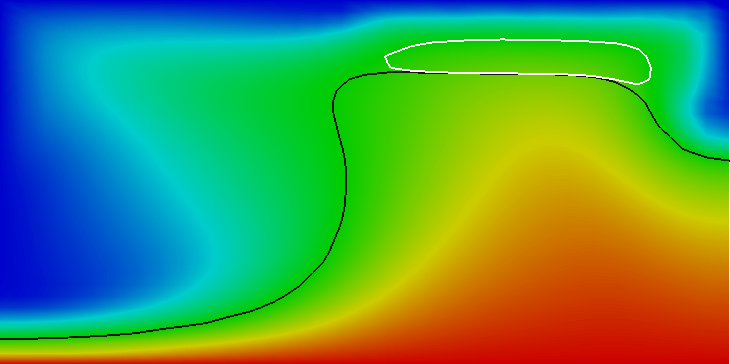
\includegraphics[width=0.4\textwidth]{viz/statistics/2.png}
  \hfill
  \phantom.
  \caption{\it Visualizing the statistics file obtained from the example in
    Section~\ref{sec:cookbooks-simple-box} using \texttt{Gnuplot}: Output
    using simple commands.}
  \label{fig:viz-gnuplot-1}
\end{figure}

For those who are lazy, \texttt{Gnuplot} allows to abbreviate things in many
different ways. For example, one can abbreviate most commands. Furthermore,
one does not need to repeat the name of an input file if it is the same
as the previous one in a plot command. Thus, instead of the commands above,
the following abbreviated form would have achieved the same effect:
\begin{lstlisting}[frame=single,language=gnuplot,showstringspaces=false]
  se xl "Time"
  se yl "Heat flux"
  se sty da lp
  pl [:0.2][-10:10] "statistics" us 2:19 t "Bottom boundary", "" us 2:20 t "Top boundary"
\end{lstlisting}
This is of course unreadable at first but becomes useful once you become
more familiar with the commands offered by this program.

Once you have gotten the commands that create the plot you want right, you probably
want to save it into a file. \texttt{Gnuplot} can write output in many
different formats. For inclusion in publications, either \texttt{eps} or
\texttt{png} are the most common. In the latter case, the commands to
achieve this are
\begin{lstlisting}[frame=single,language=gnuplot,showstringspaces=false]
  set terminal png
  set output "heatflux.png"
  replot
\end{lstlisting}
The last command will simply generate the same plot again but this time
into the given file. The result is a graphics file similar to the one
shown in Fig.~\ref{fig:convection-box-stats} on page \pageref{fig:convection-box-stats}.

\note{After setting output to a file, \textit{all} following plot commands will
  want to write to this file. Thus, if you want to create more plots after
  the one just created, you need to reset output back to the screen. On Linux,
  this is done using the command \texttt{set terminal X11}. You can then
  continue experimenting with plots and when you have the next plot ready,
  switch back to output to a file.}

What makes \texttt{Gnuplot} so useful is that it doesn't just allow entering
all these commands at the prompt. Rather, one can write them all into a file,
say \texttt{plot-heatflux.gnuplot}, and then, on the command line, call
\begin{lstlisting}[frame=single,language=ksh]
  gnuplot plot-heatflux.gnuplot
\end{lstlisting}
to generate the \texttt{heatflux.png} file. This comes in handy if one wants
to create the same plot for multiple simulations while playing with parameters
of the physical setup. It is also a very useful tool if one wants to generate
the same kind of plot again later with a different data set, for example when
a reviewer requested additional computations to be made for a paper or if one
realizes that one has forgotten or misspelled an axis label in a plot.%
\footnote{In my own work, I usually save the \aspect{} input file, the
  \texttt{statistics} output file and the \texttt{Gnuplot} script along with
  the actual figure I want to include in a paper. This way, it is easy to
  either re-run an entire simulation, or just tweak the graphic at a later
  time. Speaking from experience, you will not believe how often one wants
  to tweak a figure long after it was first created. In such situations it is
  outstandingly helpful if one still has both the actual data as well as the script
  that generated the graphic.}

\texttt{Gnuplot} has many many more features we have not even touched upon. For
example, it is equally happy to produce three-dimensional graphics, and it also
has statistics modules that can do things like curve fits, statistical regression,
and many more operations on the data you provide in the columns of an input file.
We will not try to cover them here but instead refer to the manual at
\url{http://www.gnuplot.info/}. You can also get a good amount of information
by typing \texttt{help} at the prompt, or a command like \texttt{help plot} to
get help on the \texttt{plot} command.


\subsubsection{Large data issues for parallel computations}
\label{sec:viz-data}

Among the challenges in visualizing the results of parallel computations is
dealing with the large amount of data. The first bottleneck this presents is
during run-time when \aspect{} wants to write the visualization data of a time
step to disk. Using the compressed VTU format, \aspect{} generates on the
order of 10 bytes of output for each degree of freedom in 2d and more in 3d;
thus, output of a single time step can run into the range of gigabytes that
somehow have to get from compute nodes to disk. This stresses both the cluster
interconnect as well as the data storage array.
\index[prmindex]{Number of grouped files}
\index[prmindexfull]{Postprocess!Visualization!Number of grouped files}


There are essentially two strategies supported by \aspect{} for this scenario:
\begin{itemize}
\item If your cluster has a fast interconnect, for example Infiniband, and if
  your cluster has a fast, distributed file system, then \aspect{} can produce
  output files that are already located in the correct output directory (see
  the options in Section~\ref{parameters:global}) on the global file
  system. \aspect{} uses MPI I/O calls to this end, ensuring that the local
  machines do not have to access these files using slow NFS-mounted global
  file systems.

\item If your cluster has a slow interconnect, e.g., if it is simply a
  collection of machines connected via Ethernet, then writing data to a
  central file server may block the rest of the program for a while. On the
  other hand, if your machines have fast local storage for temporary file
  systems, then \aspect{} can write data first into such a file and then move
  it in the background to its final destination while already continuing
  computations. To select this mode, set the appropriate variables discussed
  in Section~\ref{parameters:Postprocess/Visualization}. Note, however, that
  this scheme only makes sense if every machine on which MPI processes run has
  fast local disk space for temporary storage.
\end{itemize}

\note{An alternative would be if every processor directly writes its own files
  into the global output directory (possibly in the background), without the
  intermediate step of the temporary file. In our experience, file servers are
  quickly overwhelmed when encountering a few hundred machines wanting to
  open, fill, flush and close their own file via NFS mounted file system
  calls, sometimes completely blocking the entire cluster environment for
  extended periods of time.}

\subsection{Checkpoint/restart support}
\label{sec:checkpoint-restart}

If you do long runs, especially when using parallel computations, there are a
number of reasons to periodically save the state of the program:
\begin{itemize}
\item If the program crashes for whatever reason, the entire computation may
  be lost. A typical reason is that a program has exceeded the requested
  wallclock time allocated by a batch scheduler on a cluster.
\item Most of the time, no realistic initial conditions for strongly
  convecting flow are available. Consequently, one typically starts with a
  somewhat artificial state and simply waits for a long while till the
  convective state enters the phase where it shows its long-term
  behavior. However, getting there may take a good amount of CPU time and it
  would be silly to always start from scratch for each different parameter
  setting. Rather, one would like to start such parameter studies with a saved
  state that has already passed this initial, unphysical, transient stage.
\end{itemize}

To this end, \aspect{} creates a set of files in the output directory
\index[prmindex]{Output directory}
\index[prmindexfull]{Output directory}
(selected in the parameter file) every N time steps (controlled by the number
of steps or wall time as specified in \texttt{subsection Checkpointing}, see
Section~\ref{parameters:Checkpointing}) in which the entire state of the
program is saved so that a simulation can later be continued at this
point. The previous checkpoint files will then be deleted. To resume
operations from the last saved state, you need to set the \texttt{Resume
  computation} flag in the input parameter file to \texttt{true}, see
\index[prmindex]{Resume computation}
\index[prmindexfull]{Resume computation}
Section~\ref{parameters:Resume computation}.

\note{It is not imperative that the parameters selected in the input file are
  exactly the same when resuming a program from a saved state than what they
  were at the time when this state was saved. For example, one may want to
  choose a different parameterization of the material law, or add or remove
  postprocessors that should be run at the end of each time step. Likewise,
  the end time, the times at which some additional mesh refinement steps
  should happen, etc., can be different.

  Yet, it is
  clear that some other things can't be changed: For example, the geometry
  model that was used to generate the coarse mesh and describe the boundary
  must be the same before and after resuming a computation. Likewise, you can
  not currently restart a computation with a different number of processors
  than initially used to checkpoint the simulation.
  Not all invalid
  combinations are easy to detect, and \aspect{} may not always realize
  immediate what is going on if you change a setting that can't be
  changed. However, you will almost invariably get nonsensical results after
  some time.}


\subsection{Making \aspect{} run faster}

When developing \aspect{}, we are guided by the principle that the default for
all settings should be \textit{safe}. In particular, this means that you should
get errors when something goes wrong, the program should not let you choose an
input file parameter so that it doesn't make any sense, and we should solve the
equations to best ability without cutting corners. The goal is that when you
start working with \aspect{} that we give you the best answer we can. The
downside is that this also makes \aspect{} run slower than may be possible. This
section describes ways of making \aspect{} run faster -- assuming that you know
what you are doing and are making conscious decisions.

\subsubsection{Debug vs.~optimized mode}
Both \dealii{} and \aspect{} by default have a great deal of internal checking
to make sure that the code's state is valid. For example, if you write a new
postprocessing plugin (see Section~\ref{sec:plugins})) in which you need to
access the solution vector, then \dealii{}'s \texttt{Vector} class will make
sure that you are only accessing elements of the vector that actually exist and
are available on the current machine if this is a parallel computation. We do so
because it turns out that by far the most bugs one introduces in programs are of
the kind where one tries to do something that obviously doesn't make sense
(such as accessing vector element 101 when it only has 100 elements). These
kinds of bugs are more frequent than implementing a wrong algorithm, but they
are fortunately easy to find if you have a sufficient number of assertions in
your code. The downside is that assertions cost run time.

As mentioned above, the default is to have all of these assertions in the code
to catch those places where we may otherwise silently access invalid memory
locations. However, once you have a plugin running and verified that your input
file runs without problems, you can switch off all of these checks by switching
from debug to optimized mode. This means re-compiling \aspect{} and linking
against a version of the \dealii{} library without all of these internal checks.
Because this is the first thing you will likely want to do, we have already
discussed how to do all of this in Section~\ref{sec:debug-mode}.

\subsubsection{Adjusting solver tolerances} At the heart of every time step
lies the solution of linear systems for the Stokes equations, the temperature
field, and possibly for compositional fields. In essence, each of these steps
requires us to solve a linear system of the form $Ax=b$ which we do through
iterative solvers, i.e., we try to find a sequence of approximations $x^{(k)}$
where $x^{(k)}\rightarrow x=A^{-1}b$. This iteration is terminated at iteration
$k$ if the approximation is ``close enough'' to the exact solution. The solvers
we use determine this by testing after every iteration whether the
\textit{residual}, $r^{(k)}=A(x-x^{(k)})=b-Ax^{(k)}$, satisfies
$\|r^{(k)}\|\le\varepsilon\|r^{(0)}\|$ where $\varepsilon$ is called the
(relative) \textit{tolerance}.

Obviously, the smaller we choose $\varepsilon$, the more accurate the
approximation $x^{(k)}$ will be. On the other hand, it will also take more
iterations and, consequently, more CPU time to reach the stopping criterion with
a smaller tolerance. The default value of these tolerances are chosen so that
the approximation is typically sufficient. You can make \aspect{} run faster if
you choose these tolerances larger.
The parameters you can adjust are all listed in
Section~\ref{parameters:Solver_20parameters} and are located in the \texttt{Solver parameters} subsection of the input
file. In particular, the parameters you want to look at are \texttt{Linear
solver tolerance}, \texttt{Temperature solver tolerance} and
\texttt{Composition solver tolerance}.
\index[prmindex]{Composition solver tolerance}
\index[prmindexfull]{Composition solver tolerance}
\index[prmindex]{Linear solver tolerance}
\index[prmindexfull]{Linear solver tolerance}
\index[prmindex]{Temperature solver tolerance}
\index[prmindexfull]{Temperature solver tolerance}

All this said, it is important to understand the consequences of choosing
tolerances larger. In particular, if you choose tolerances too large, then the
difference between the exact solution of a linear system $x$ and the
approximation $x^{(k)}$ may become so large that you do not get an accurate
output of your model any more. A rule of thumb in choosing tolerances is to
start with a small value and then increase the tolerance until you come to a
point where the output quantities start to change significantly. This is the
point where you will want to stop.

\subsubsection{Adjusting solver preconditioner tolerances} To solve the Stokes
equations it is necessary to lower the condition number of the
Stokes matrix by preconditioning  it. In \aspect{} a right preconditioner $Y^{-1} =
\begin{pmatrix}
\widetilde{A^{-1}} & -\widetilde{A^{-1}}B^{T}\widetilde{S^{-1}} \\
0 & \widetilde{S^{-1}}
\end{pmatrix}$ is used to precondition the system, where $\widetilde{A^{-1}}$ is
the approximate inverse of the A block and $\widetilde{S^{-1}}$ is the approximate
inverse of the Schur complement matrix. Matrix $\widetilde{A^{-1}}$ and
$\widetilde{S^{-1}}$ are calculated through a CG solve, which requires a tolerance
to be set. In comparison with the solver tolerances of the previous section, these
parameters are relatively safe to use, since they only change the preconditioner,
but can speed up or slow down solving the Stokes system considerably.

In practice $\widetilde{A^{-1}}$ takes by far the most time to compute, but is
also very important in conditioning the system. The accuracy of the computation
of $\widetilde{A^{-1}}$ is controlled by the parameter \texttt{Linear solver A
block tolerance} which has a default value of $1e-2$. Setting this tolerance
to a less strict value will result in more outer iterations, since the
preconditioner is not as good, but the amount of time to compute
$\widetilde{A^{-1}}$ can drop significantly resulting in a reduced total solve
time. The cookbook crustal deformation (Section
\ref{sec:cookbooks-crustal-deformation}) for example can be computed much faster
by setting the \texttt{Linear solver A block tolerance} to $5e-1$. The
calculation of $\widetilde{S^{-1}}$ is usually much faster and the
conditioning of the system is less sensitive to the parameter \texttt{Linear
solver S block tolerance}, but for some problems it might be worth it to
investigate.
\index[prmindex]{Linear solver A block tolerance}
\index[prmindexfull]{Linear solver A block tolerance}
\index[prmindex]{Linear solver S block tolerance}
\index[prmindexfull]{Linear solver S block tolerance}

\subsubsection{Using lower order elements for the temperature/compositional discretization}
The default settings of \aspect{} use quadratic finite elements for the
velocity. Given that the temperature and compositional fields essentially (up
to material parameters) satisfy advection equations of the kind $\partial_t T +
\mathbf u \cdot \nabla T = \ldots$, it seems appropriate to also use quadratic
finite element shape functions for the temperature and compositional fields.

However, this is not mandatory. If you do not care about high accuracy in these
fields and are mostly interested in the velocity or pressure field, you can
select lower-order finite elements in the input file. The polynomial degrees are
controlled with the parameters in the \textit{discretization} section of the
input file, see Section~\ref{parameters:Discretization}, in particular by
\texttt{Temperature polynomial degree} and
\texttt{Composition polynomial degree}.
\index[prmindex]{Temperature polynomial degree}
\index[prmindexfull]{Discretization!Temperature polynomial degree}
\index[prmindex]{Composition polynomial degree}
\index[prmindexfull]{Discretization!Composition polynomial degree}

As with the other parameters discussed above and below, it is worthwhile
comparing the results you get with different values of these parameters when
making a decision whether you want to save on accuracy in order to reduce
compute time. An example of how this choice affects the accuracy you get is
discussed in Section~\ref{sec:cookbooks-simple-box}.



\subsubsection{Limiting postprocessing}
\aspect{} has a lot of postprocessing capabilities, from generating graphical
output to computing average temperatures or temperature fluxes. To see what all
is possible, take a look at the \texttt{List of postprocessors} parameter that
can be set in the input file, see Section~\ref{parameters:Postprocess}.
\index[prmindex]{List of postprocessors}
\index[prmindexfull]{Postprocess!List of postprocessors}

Many of these postprocessors take a non-negligible amount of time. How much they
collectively use can be inferred from the timing report \aspect{} prints
periodically among its output, see for example the output shown in
Section~\ref{sec:cookbooks-simple-box}. So, if your computations take too long,
consider limiting which postprocessors you run to those you really need. Some
postprocessors -- for example those that generate graphical output, see
Section~\ref{parameters:Postprocess/Visualization} -- also allow you to run them
only once every once in a while, rather than at every time step.


\subsubsection{Switching off pressure normalization}
In most practically relevant cases, the Stokes equations
\eqref{eq:stokes-1}--\eqref{eq:stokes-2} only determine the pressure up to a
constant because only the pressure gradient appears in the equations, not the
actual value of it. However, unlike this ``mathematical'' pressure, we have a
very specific notion of the ``physical'' pressure: namely a well-defined
quantity that at the surface of Earth equals the air pressure, which compared to
the hydrostatic pressure inside Earth is essentially zero.

As a consequence, the default in \aspect{} is to normalize the computed
``mathematical'' pressure in such a way that either the mean pressure at the
surface is zero (where the geometry model describes where the ``surface'' is,
see Section~\ref{sec:geometry-models}), or that the mean pressure in the domain
is zero. This normalization is important if your model describes densities,
viscosities and other quantities in dependence of the pressure -- because you
almost certainly had the ``physical'' pressure in mind, not some unspecified
``mathematical'' one. On the other hand, if you have a material model in which
the pressure does not enter, then you don't need to normalize the pressure at
all -- simply go with whatever the solver provides. In that case, you can switch
off pressure normalization by looking at the \texttt{Pressure normalization}
parameter at the top level of the input file, see
Section~\ref{parameters:global}.
\index[prmindex]{Pressure normalization}
\index[prmindexfull]{Pressure normalization}


\subsubsection{Regularizing models with large coefficient variation}
Models with large jumps in viscosity and other coefficients present
significant challenges to both discretizations and solvers. In particular,
they can lead to very long solver
times. Section~\ref{sec:sinker-with-averaging} presents parameters that can
help regularize models and these typically also include significant
improvements in run-time.
\index[prmindex]{Material averaging}
\index[prmindexfull]{Material model!Material averaging}


\subsubsection{Using multithreading}
In most cases using as many MPI processes as possible is the optimal
parallelization strategy for \aspect{} models, but if you are limited by the
amount of MPI communication it can be beneficial to use multiple threads per
MPI process. While not utilized by our linear solvers, this parallelization can
speed up the assembly of the system matrices, e.g. by around 10-15\% if you
utilize unused logical cores, or nearly linearly if you use otherwise
unused physical cores. This can also reduce the performance cost if you are
memory limited and need to run your model on less than the available number of
cores per node on a cluster to increase the available memory per core.  Running
with for example two threads per process will offset some of the performance
loss you will see in these situations.

Multithreading is controlled by setting the command line parameter \texttt{-j}
or \texttt{-{}-threads}. If the parameter is not set, \aspect{} will create
exactly one thread per MPI process, i.e. multithreading is disabled.  Appending
the parameter allows \aspect{} to spawn several threads per MPI process. Note
that the internally used TBB library will determine the number of threads based
on the number of available cores, i.e., if you start 2~MPI processes on a
quadcore machine with hyperthreading (8 logical cores), \aspect{} will spawn 4
threads on each MPI process. Also note that there is no guarantee that the
final number of threads will exactly match the number of available logical
cores if you start with a number of processes that is not a divisor of your
logical cores (e.g. 3 MPI processes for 8 logical cores).

\subsection{Input parameter files}
\label{sec:parameters-overview}

What \aspect{} computes is driven by two things:
\begin{itemize}
\item The models implemented in \aspect{}. This includes the geometries, the
  material laws, or the initial conditions currently supported. Which of these
  models are currently implemented is discussed below;
  Section~\ref{sec:extending} discusses in great detail the process of
  implementing additional models.

\item Which of the implemented models is selected, and what their run-time
  parameters are. For example, you could select a model that prescribes
  constant coefficients throughout the domain from all the material models
  currently implemented; you could then select appropriate values for all of
  these constants. Both of these selections happen from a parameter file that
  is read at run time and whose name is specified on the command line. (See
  also Section~\ref{sec:running-overview}.)
\end{itemize}
In this section, let us give an overview of what can be selected in the
parameter file. Specific parameters, their default values, and allowed values
for these parameters are documented in Section~\ref{sec:parameters}. An index
with page numbers for all run-time parameters can be found on
page~\pageref{sec:runtime-parameter-index}.

\subsubsection{The structure of parameter files}

Most of the run-time behavior of \aspect{} is driven by a parameter file that
looks in essence like this:
\lstinputlisting[language=prmfile]{cookbooks/overview/doc/structure.part.prm.out}

Some parameters live at the top level, but most parameters are grouped into
subsections. An input parameter file is therefore much like a file system: a
few files live in the root directory; others are in a nested hierarchy of
sub-directories. And just as with files, parameters have both a name (the
thing to the left of the equals sign) and a content (what's to the right).

All parameters you can list in this input file have been \textit{declared} in
\aspect. What this means is that you can't just list anything in the input
file, and expect that entries that are unknown are simply ignored.
Rather, if your input file contains a line setting a parameter that is unknown, you
will get an error message. Likewise, all declared parameters have a
description of possible values associated with them -- for example, some
parameters must be non-negative integers (the number of initial refinement
steps), can either be true or false (whether the computation should be resumed
from a saved state), or can only be a single element from a selection (the
name of the material model). If an entry in your input file doesn't satisfy
these constraints, it will be rejected at the time of reading the file (and
not when a part of the program actually accesses the value and the programmer
has taken the time to also implement some error checking at this location).
Finally, because parameters have been declared, you do not \textit{need} to
specify a parameter in the input file: if a parameter isn't listed, then the
program will simply use the default provided when declaring the parameter.

\note{In cases where a parameter requires a significant amount of text, you can
end a line in the input file with a backslash. This indicates that the
following line will simply continue to be part of the text of the current line,
in the same way as the C/C++ preprocessor expands lines that end in
backslashes. The underlying implementation always eats whitespace at
the beginning of each continuing line, but not before the
backslash. This means that the parameter file \\
\hspace*{.25cm} \texttt{set Some parameter = abc}$\backslash$ \\
\hspace*{.25cm} \texttt{\phantom{set Some parameter = }def}\\
is equivalent to \\
\hspace*{.25cm} \texttt{set Some parameter = abcdef}\\
that is, with no space between \texttt{abc} and \texttt{def} despite
the leading whitespace at the beginning of the second line. If you
do want space between these two parts, you need to add it before the
backslash in the first of the two lines.
}

\subsubsection{Categories of parameters}

The parameters that can be provided in the input file can roughly be
categorized into the following groups:
\begin{itemize}
\item Global parameters (see Section~\ref{parameters:global}): These
  parameters determine the overall behavior of the program. Primarily they
  describe things like the output directory, the end time of the simulation,
  or whether the computation should be resumed from a previously saved state.

\item Parameters for certain aspects of the numerical algorithm: These
  describe, for example, the specifics of the spatial discretization. In
  particular, this is the case for parameters concerning
  the polynomial degree of the finite element approximation
  (Section~\ref{parameters:Discretization}), some details about the
  stabilization
  (Section~\ref{parameters:Discretization/Stabilization_20parameters}), and
  how adaptive mesh refinement is supposed to work
  (Section~\ref{parameters:Mesh_20refinement}).

\item Parameters that describe certain global aspects of the equations to be
  solved: This includes, for example, a description if certain terms in the
  model should be omitted or not. See
  Section~\ref{parameters:Formulation} for the list of parameters in this
  category.

\item Parameters that characterize plugins: Certain behaviors of
  \aspect{} are described by what we call \textit{plugins} -- self-contained
  parts of the code that describe one particular aspect of the simulation. An
  example would be which of the implemented material models to use, and the
  specifics of this material model. The sample parameter file above gives an
  indication of how this works: within a subsection of the file that pertains
  to the material models, one can select one out of several plugins (or, in
  the case of the postprocessors, any number, including none, of the available
  plugins), and one can then specify the specifics of this model in a
  sub-subsection dedicated to this particular model.

  A number of components of \aspect{} are implemented via plugins. Some of
  these, together with the sections in which their parameters are declared, are
  the following:
  \begin{itemize}
  \item The material model:
    Sections~\ref{parameters:Material_20model} and following.
  \item The geometry:
    Sections~\ref{parameters:Geometry_20model} and following.
  \item The gravity description:
    Sections~\ref{parameters:Gravity_20model} and following.
  \item Initial conditions for the temperature:
    Sections~\ref{parameters:Initial_20temperature_20model} and following.
  \item Temperature boundary conditions:
    Sections~\ref{parameters:Boundary_20temperature_20model} and following.
  \item Postprocessors:
    Sections~\ref{parameters:Postprocess} and following for most postprocessors,
    section \ref{parameters:Postprocess/Visualization} and following for
    postprocessors related to visualization.
  \end{itemize}
\end{itemize}

The details of parameters in each of these categories can be found in the
sections linked to above. Some of them will also be used in the cookbooks in
Section~\ref{sec:cookbooks}.


\subsubsection{A note on the syntax of formulas in input files}
\label{sec:muparser-format}

Input files have different ways of describing certain things to \aspect{}. For
example, you could select a plugin for the temperature initial values that
prescribes a constant temperature, or a
plugin that implements a particular formula for these initial conditions in
C++ in the code of the plugin, or a
plugin that allows you to describe this formula in a symbolic way in the input file
(see Section~\ref{parameters:Initial_20temperature_20model}). An example of this latter
case is this snippet of code discussed in
Section~\ref{sec:cookbooks-simple-box-3d}:
%
\lstinputlisting[language=prmfile]{../../cookbooks/convection_box_3d/doc/initial.part.prm.out}
%
The formulas you can enter here need to use a syntax that is understood by the
functions and classes that interpret what you write. Internally, this is done
using the muparser library, see \url{http://muparser.beltoforion.de/}. The
syntax is mostly self-explanatory in that it allows to use the usual symbols
\texttt{x}, \texttt{y} and \texttt{z} to reference coordinates (unless a
particular plugin uses different variables, such as the depth), the symbol
\texttt{t} for time in many situations, and allows you to use all of the
typical mathematical functions such as sine and cosine. Based on the muparser
library, deal.II supports additional functions, including \texttt{|} (the logical OR), \texttt{\&} (the logical AND),
\texttt{int()}, \texttt{ceil()}, \texttt{floor()}, \texttt{cot()},
\texttt{csc()}, \texttt{sec()}, \texttt{pow()}, \texttt{log()},
\texttt{erfc()}, \texttt{rand()}, and \texttt{rand\_seed()}.
For more detailed information, see
\url{http://www.dealii.org/developer/doxygen/deal.II/classFunctionParser.html#details}.

A common need for function expression is an if-else-statement, for example
``if $1<x<4$ then output 1, else output 0''.
The muparser uses lazy-expression syntax \texttt{(if-condition ?\ true-expression :\ false-expression )}
for if-else statements. This lazy-expression only evaluates the expression that meets the
if-condition, rather than evaluating both expressions, which can be useful if one of the
expressions is not defined (e.g., has a divide by zero) when the if-condition is not met.
Note it is also possible to use the syntax \texttt{if(condition, true-expression, false-expression)},
but in this case both expressions are always evaluated. This is inefficient, but in addition may abort the program with a floating point exception if the expression that will be discarded has invalid floating point operations (such as a division by zero, or taking the square root of a negative number) that would ordinarily not be visible because, after all, the expression should be discarded.
Therefore, the lazy-expression syntax is recommended.

As a simple example using the lazy-expression syntax, the statement ``if $1<x<4$ then output 1, else output 0''
can be expressed as \texttt{(1<x\ \&\&\ x<4 ?\ 1\ :\ 0)}.  Multiple, nested if-else expressions
can also be used. To extend the simple example, the statement
``if $1<x<4$ then, if 2<y<3, then output 2, else output 1, else output 0''
can be expressed as \texttt{((1<x\ \&\&\ x<4)\ ?\ ((2<y\ \&\&\ y<3)\ ?\ 2\ :\ 1)\ :\ (0))}.

An example for how to translate nested if-else statements into the lazy-expression syntax is given in the
cookbook example found in Section~\ref{sec:lazy-expression}. This cookbook includes a python script that defines
the initial temperature structure using nested if-else statements and shows how this is then rewritten
using the lazy-expression. The cookbook runs a single time-step to show the outcome of using the function
option for the initial temperature. Quite complex initial conditions can be defined in this way, however,
using something like python to debug these expressions before defining them in the parameter file is
recommended. For more examples of functions used in parameter files, go to the \texttt{cookbooks}
directory and use grep to search for ``Function expression'' in the parameters files.
You can also search ``Function expression'' on the \aspect{} github page.
For more examples of the syntax understood, reference the documentation of the muparser library
linked to above.

\subsubsection{Compatibility of input files with newer \aspect{} versions}

We strive to maintain compatibility for options in input files as long as
possible. However, occasionally we have to reorder, rename, or remove options
from parameter files to improve \aspect{} further. This is especially true
for new major versions. In order to allow running old parameter files with
newer \aspect{} versions we provide scripts that can automatically update
existing parameter files to the new syntax. Executing
\texttt{doc/update\_prm\_files.sh} with one or more parameter files as
arguments will create a backup of the old parameter file (named
\texttt{old\_filename.bak}), and replace the existing file with a version that
should work with the current \aspect{} version. Using this script would look
like this:

\begin{lstlisting}[frame=single,language=ksh,showstringspaces=false]
bash contrib/utilities/update_prm_files.sh cookbooks/convection_box.prm
\end{lstlisting}

\note{Not all text replacements are unique, and the structure of input files
allows for constructions the script can not properly parse. Also we can not
guarantee to preserve the structure and position of comments, as it is not
always clear to which part of the input file they refer. Thus, it is important
that you check your updated input file for errors. That being said, all input
files in the main \aspect{} repository are updated successfully using this
script.}

\subsection{A graphical user interface for editing \aspect{} parameter files}
Preparing a parameter file in a text editor can be a tedious task, not
only because the number of input parameters has grown considerably during the
development of \aspect{}, but also because remembering the names of commonly
used options is a waste of (human) memory. Therefore, we provide a graphical
user interface that builds upon an available program for \dealii{}. This GUI
allows to investigate existing input parameters, including their default values, modify
these values in a spreadsheet like environment and then save a formatted
parameter file that can be used to start an ASPECT model. In the following
subsections we describe installing and using this user interface.

\subsubsection{Installing parameter-GUI}
The \dealii{} parameter-GUI program can be downloaded at \url{https://github.com/dealii/parameter_gui},
and is compiled using the \texttt{cmake} program just like \aspect{} itself. The program has no
dependencies except for the Qt development libraries that should be available as packages for
most Linux distributions and can also be obtained for all major operating systems at
\url{https://www.qt.io/download-open-source/}.

Example steps for installing the parameter-gui could look as follows:
\begin{enumerate}
\item Download the program from \url{https://github.com/dealii/parameter_gui}.
\item Prepare a Makefile by running \texttt{cmake .} in the source folder.
\item Compile the program by running \texttt{make}.
\item Make sure to set the environment variable \texttt{PARAMETER\_GUI\_DIR}
to the directory that contains the parameter-GUI executable (optional).
This will allow \aspect{} to automatically enable the GUI during configuration.
\end{enumerate}

\paragraph{Installing on macOS} On a mac machine with recent macOS Sierra 10.12.4, Qt development libraries of version 4.x.x at the libraries' official website \url{https://www.qt.io/download-open-source/} may fail to install.  Alternatively, you can install \texttt{qt4} through Homebrew (also see instruction here \url{https://github.com/cartr/homebrew-qt4})
\begin{verbatim}
brew tap cartr/qt4
brew tap-pin cartr/qt4
brew install qt@4
\end{verbatim}
or install it through Mac Ports (\url{https://www.macports.org/})
\begin{verbatim}
sudo port install qt4-mac
\end{verbatim}
Then you can follow the Linux user instructions provided previously to download and install dealii parameter-GUI.
Before running \texttt{cmake .}, you may need to either pass the path of \texttt{qt4} and specify the value of variable \texttt{QT\_LIBRARIES} to the directory that contains the libraries of \texttt{qt4}
or add those information into your \texttt{.bash\_profile}. For example, for installation through Mac Ports, you can set the following into your \texttt{.bash\_profile}
\begin{verbatim}
export PATH="$PATH:/opt/local/libexec/qt4"
export QT_LIBRARIES="/opt/local/libexec/qt4"
\end{verbatim}




\subsubsection{Using \aspect{}-GUI}

When configuring \aspect{} after executing the above steps, it should automatically pick up the
location of the parameter-GUI, and will create a new script named \texttt{aspect-gui} within the build folder.
If this does not happen, it is possible to hand over the location of the parameter-GUI as a cmake
variable during configuration (e.g. \texttt{cmake -D PARAMETER\_GUI\_EXECUTABLE=path\_to\_your\_executable}).

The aspect-gui script can be executed from any folder either with no argument or with one argument that contains the path to
an existing parameter file. The script will run \aspect{} with the given (or an empty) parameter file, generate a database
of existing input parameters, and open the parameter-GUI program with this database. The resulting window looks similar to Fig.~\ref{fig:aspect-gui}. If an existing parameter file was
given, all parameter fields are pre-filled with the values set in the file instead of the default values.
In the program's main window you can change parameters as necessary, and then save the file as a new parameter file. This parameter file can then be used
to start an \aspect{} model as usual. Note that it is possible to prepare and execute the parameter file with different versions of \aspect{}, e.g. if you prepare parameter files on a local machine, and execute the model on a remote compute cluster.
Note however that if the two \aspect{} versions contain different default values or parameter names have changed, this can lead
to unexpected model behavior or even unusable parameter files.

\begin{figure}
\hfill
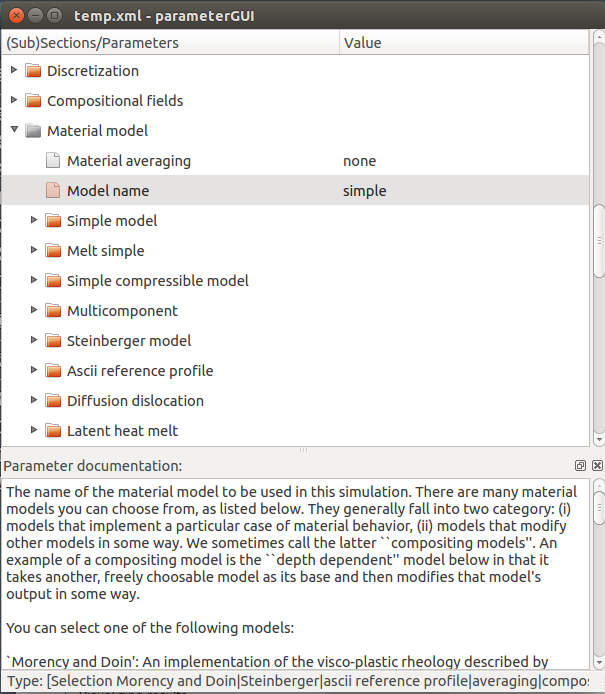
\includegraphics[width=0.4\textwidth]{aspect-gui.png}
\hfill
\phantom.
\caption{\it The parameter GUI lists all available parameter options, and allows to change and save them into a new parameter file. Input fields know about the type of the variable and will display useful options to change them (e.g. drop-down menus, file dialogs, text fields).}
\label{fig:aspect-gui}
\end{figure}

\section{Cookbooks}
\label{sec:cookbooks}

In this section, let us present a number of ``cookbooks'' -- examples of how
to use \aspect{} in typical or less typical ways. As discussed in
Sections~\ref{sec:running} and \ref{sec:parameters}, \aspect{} is driven by
run-time parameter files, and so setting up a particular situation primarily
comes down to creating a parameter file that has the right entries. Thus, the
subsections below will discuss in detail what parameters to set and to what
values. Note that parameter files need not specify \textit{all} parameters --
of which there is a bewildering number -- but only those that are relevant to
the particular situation we would like to model. All parameters not listed
explicitly in the input file are simply left at their default value (the
default values are also documented in Section~\ref{sec:parameters}).

Of course, there are situations where what you want to do is not covered by
the models already implemented. Specifically, you may want to try a different
geometry, a different material or gravity model, or different boundary
conditions. In such cases, you will need to implement these extensions in the
actual source code. Section~\ref{sec:extending} provides information on how to
do that.

The remainder of this section shows a number of applications of
\aspect{}. They are grouped into three categories: Simple setups of examples
that show thermal convection (Section~\ref{sec:cookbooks-simple}), setups
that try to model geophysical situations (Section~\ref{sec:cookbooks-geophysical})
and setups that are used to benchmark \aspect{} to ensure correctness or to test accuracy
of our solvers (Section~\ref{sec:cookbooks-benchmarks}). Before we get there,
however, we will review how one usually approaches setting up computations in
Section~\ref{sec:cookbooks-overview}.

\note{The input files discussed in the following sections can generally be
  found in the \texttt{cookbooks/} directory of your \aspect{} installation.}


\subsection{How to set up computations}
\label{sec:cookbooks-overview}

\aspect{}'s computations are controlled by input parameter files such as those
we will discuss in the following sections.%
\footnote{You can also extend \aspect{} using plugins -- i.e., pieces of code
you compile separately and either link into the \aspect{} executable itself, or
reference from the input file. This is discussed in
Section~\ref{sec:extending}.}
Basically, these are just regular text files you can edit with programs like
\texttt{gedit}, \texttt{kwrite} or \texttt{kate} when working on Linux, or
something as simple as \texttt{NotePad} on Windows. When setting up these input
files for a model you have in mind, you have to describe everything
that characterizes the situation you are considering. In particular,
this includes the following:
\begin{itemize}
  \item What internal forces act on the medium (the equation)?
  \item What external forces do we have (the right hand side)
  \item What is the domain (geometry)?
  \item What happens at the boundary for each variable involved (boundary
 conditions)?
  \item How did it look at the beginning (initial conditions)?
\end{itemize}
For each of these questions, there are one or more input parameters (sometimes
grouped into sections) that allow you to specify what you want. For example, to
choose a geometry, you will typically have a block like this in your input file:
%
\lstinputlisting[language=prmfile]{cookbooks/overview/doc/geometry.part.prm.out}
%
This indicates that you want to do a computation in 2d, using a rectangular
geometry (a ``box'') with edge length equal to one in both the $x$- and
$y$-directions. Of course, there are other geometries you can choose from for
the \texttt{Model name} parameter, and consequently other subsections that
specify the details of these geometries.

Similarly, you describe boundary conditions using parameters such as this:
%
\lstinputlisting[language=prmfile]{cookbooks/overview/doc/boundary-conditions.part.prm.out}
%
This snippet describes which of the four boundaries of the two-dimensional box
we have selected above should have a prescribed temperature or an insulating
boundary, and at which parts of the boundary we want zero, tangential or
prescribed velocities.%
\footnote{Internally, the geometry models \aspect{} uses label every part of
  the boundary with what is called a \textit{boundary indicator} -- a number
  that identifies pieces of the boundary. If you know which number each piece
  has, you can list these numbers on the right hand sides of the assignments
  of boundary types above. For example, the left boundary of the box has
  boundary indicator zero (see Section~\ref{parameters:Geometry_20model}), and
  using this number instead of the \texttt{left} would have been equally
  valid. However, numbers are far more difficult to remember than names, and
  consequently every geometry model provides string aliases such as
  ``\texttt{left}'' for each boundary indicator describing parts of the
  boundary. These symbolic aliases are specific to the geometry -- for the
  box, they are ``\texttt{left}'', ``\texttt{right}'', ``\texttt{bottom}'',
  etc., whereas for a spherical shell they are ``\texttt{inner}'' and
  ``\texttt{outer}'' -- but are described in the documentation of every
  geometry model, see Section~\ref{parameters:Geometry_20model}.}

If you go down the list of questions about the setup above, you have already
done the majority of the work describing your computation. The remaining
parameters you will typically want to specify have to do with the computation
itself. For example, what variables do you want to output and how often? What
statistics do you want to compute. The following sections will give ample
examples for all of this, but using the questions above as a guideline is
already a good first step.

\note{It is of course possible to set up input files for computations
completely from scratch. However, in practice, it is often simpler to go
through the list of cookbooks already provided and find one that comes close to
what you want to do. You would then modify this cookbook until it does what you
want to do. The advantage is that you can start with something you already know
works, and you can inspect how each change you make -- changing the
details of the geometry, changing the material model, or changing what is being
computed at the end of each time step -- affects what you get.}


\subsection{Simple setups}
\label{sec:cookbooks-simple}

\include*{cookbooks/convection-box/doc/convection-box.tex}

% cookbooks/convection_box_3d
\include*{cookbooks/convection_box_3d/doc/convection_box_3d.tex}


% cookbooks/platelike-boundary
\include*{cookbooks/platelike-boundary/doc/platelike-boundary.tex}


\subsubsection{Using passive and active compositional fields}
\label{sec:cookbooks-composition}

One frequently wants to track where material goes, either because one simply
wants to see where stuff ends up (e.g., to determine if a particular model
yields mixing between the lower and upper mantle) or because the material model
in fact depends not only pressure, temperature and location but also on the
mass fractions of certain chemical or other species. We will refer to the first
case as \textit{passive} and the latter as \textit{active} to indicate the role
of the additional quantities whose distribution we want to track. We refer to
the whole process as \textit{compositional} since we consider quantities that
have the flavor of something that denotes the composition of the material at any
given point.

There are basically two ways to achieve this: one can advect a set of
particles (``tracers'') along with the velocity field, or one can advect along a
field. In the first case, where the closest particle came from indicates the
value of the concentration at any given position. In the latter case, the
concentration(s) at any given position is simply given by the value of the
field(s) at this location.

\aspect{} implements both strategies, at least to a certain degree. In this
cookbook, we will follow the route of advected fields.


% cookbooks/composition_active/

\include*{cookbooks/composition_passive/doc/composition_passive.tex}


% cookbooks/composition_active/

\include*{cookbooks/composition_active/doc/composition_active.tex}


% cookbooks/composition-reaction
\include*{cookbooks/composition-reaction/doc/composition-reaction.tex}


\subsubsection{Using particles}
\label{sec:cookbooks-particles}

Using compositional fields to trace where material has come from or is going to
has many advantages from a computational point of view. For example, the
numerical methods to advect along fields are well developed and we can do so at
a cost that is equivalent to one temperature solve for each of the compositional
fields. Unless you have many compositional fields, this cost is therefore
relatively small compared to the overall cost of a time step. Another advantage
is that the value of a compositional field is well defined at every point within
the domain. On the other hand, compositional fields over time diffuse initially
sharp interfaces, as we have seen in the images of the previous section.

At the same time, the geodynamics community has a history of using particles for
this purpose. Historically, this may have been because it is conceptually
simpler to advect along individual particles rather than whole fields, since it
only requires an ODE integrator rather than the stabilization techniques
necessary to advect fields. They also provide the appearance of no diffusion,
though this is arguable. Leaving aside the debate whether fields or particles are the
way to go, \aspect{} supports both: using fields and using particles.


% cookbooks/composition_passive_particles/

\include*{cookbooks/composition_passive_particles/doc/composition_passive_particles.tex}


% cookbooks/composition_active_particles/

\include*{cookbooks/composition_active_particles/doc/composition_active_particles.tex}


% cookbooks/free_surface
\include*{cookbooks/free_surface/doc/free_surface.tex}


% cookbooks/free_surface_with_crust
\include*{cookbooks/free_surface_with_crust/doc/free_surface_with_crust.tex}


% cookbooks/sinker-with-averaging
\include*{cookbooks/sinker-with-averaging/doc/sinker-with-averaging.tex}


% cookbooks/prescribed_velocity
\include*{cookbooks/prescribed_velocity/doc/prescribed_velocity.tex}


% cookbooks/prescribed_velocity_ascii_data
\include*{cookbooks/prescribed_velocity_ascii_data/doc/prescribed_velocity_ascii_data.tex}


% cookbooks/shell_simple_2d_smoothing
\include*{cookbooks/shell_simple_2d_smoothing/doc/shell_simple_2d_smoothing.tex}


% cookbooks/finite_strain/
\include*{cookbooks/finite_strain/doc/finite_strain.tex}

% cookbooks/geomio
\include*{cookbooks/geomio/doc/geomio.tex}


% cookbooks/muparser_temperature_example
\include*{cookbooks/muparser_temperature_example/doc/muparser_temperature_example.tex}


\include*{cookbooks/christensen_yuen_phase_function/doc/christensen_yuen_phase_function.tex}


% cookbooks/phase_diagram/
\include*{cookbooks/visualizing_phase_diagram/doc/visualizing_phase_diagram.tex}


% cookbooks/plume_2D_chunk
\include*{cookbooks/plume_2D_chunk/doc/plume.tex}


\subsection{Geophysical setups}
\label{sec:cookbooks-geophysical}

Having gone through the ways in which one can set up problems in rectangular
geometries, let us now move on to situations that are directed more towards the
kinds of things we want to use \aspect{} for: the simulation of convection in
the rocky mantles of planets or other celestial bodies.

To this end, we need to go through the list of issues that have to be described
and that were outlined in Section~\ref{sec:cookbooks-overview}, and address them
one by one:
\begin{itemize}
  \item \textit{What internal forces act on the medium (the equation)?}
    This may in fact be the most difficult to answer part of it all. The real
    material in Earth's mantle is certainly no Newtonian fluid where the stress
    is a linear function of the strain with a proportionality constant (the
    viscosity) $\eta$ that only depends on the temperature. Rather, the
    real viscosity almost surely also depends on the pressure and the strain
    rate. Because the issue is complicated and the exact material model not
    entirely clear, for the next few subsections we will therefore ignore the
    issue and start with just using the ``simple'' material model where the
    viscosity is constant and most other coefficients depend at most on the
    temperature.

  \item \textit{What external forces do we have (the right hand side)}
    There are of course other issues: for example, should the model include terms
    that describe shear heating? Should it be compressible? Adiabatic heating due
    to compression? Most of the terms that pertain to these questions appear on
    the right hand sides of the equations, though some (such as the
    compressibility) also affect the differential operators on the left. Either
    way, for the moment, let us just go with the simplest models and come back to
    the more advanced questions in later examples.

    One right hand side that will certainly be there is that due to gravitational
    acceleration. To first order, within the mantle gravity points radially
    inward and has a roughly constant magnitude. In reality, of course, the
    strength and direction of gravity depends on the distribution and density of
    materials in Earth -- and, consequently, on the solution of the model at
    every time step. We will discuss some of the associated issues in the
    examples below.

  \item \textit{What is the domain (geometry)?}
    This question is easier to answer. To first order, the domains we want to
    simulate are spherical shells, and to second order ellipsoid shells that can
    be obtained by considering the isopotential surface of the gravity field of
    a homogeneous, rotating fluid.
    A more accurate description is of course the geoid for which several
    parameterizations are available. A complication arises if we ask whether we
    want to include the mostly rigid crust in the domain and simply assume that
    it is part of the convecting mantle, albeit a rather viscous part due to its
    low temperature and the low pressure there, or whether we want to truncate
    the computation at the asthenosphere.

  \item \textit{What happens at the boundary for each variable involved
      (boundary conditions)?}
    The mantle has two boundaries: at the bottom where it contacts the outer core
    and at the top where it either touches the air or, depending on the outcome
    of the discussion of the previous question, where it contacts the
    lithospheric crust. At the bottom, a very good approximation of what is
    happening is certainly to assume that the velocity field is tangential
    (i.e., horizontal) and without friction forces due to the very low viscosity
    of the liquid metal in the outer core. Similarly, we can assume that the
    outer core is well mixed and at a constant temperature. At the top boundary,
    the situation is slightly more complex because in reality the boundary is not
    fixed but also allows vertical movement. If we ignore this, we can assume
    free tangential flow at the surface or, if we want, prescribe the tangential
    velocity as inferred from plate motion models. \aspect{} has a plugin that
    allows to query this kind of information from the \texttt{GPlates} program.

  \item \textit{How did it look at the beginning (initial conditions)?}
    This is of course a trick question. Convection in the mantle of earth-like
    planets did not start with a concrete initial temperature distribution when
    the mantle was already fully formed. Rather, convection already happened
    when primordial material was still separating into mantle and core. As a
    consequence, for models that only simulate convection using mantle-like
    geometries and materials, no physically reasonable initial conditions are
    possible that date back to the beginning of Earth. On the other hand, recall
    that we only need initial conditions for the temperature (and, if
    necessary, compositional fields). Thus, if we have a temperature profile at
    a given time, for example one inferred from seismic data at the current
    time, then we can use these as the starting point of a simulation.
\end{itemize}

This discussion shows that there are in fact many pieces with which one can play
and for which the answers are in fact not always clear. We will address some of
them in the cookbooks below. Recall in the descriptions we use in the input
files that \aspect{} uses physical units, rather than non-dimensionalizing
everything. The advantage, of course, is that we can immediately compare outputs
with actual measurements. The disadvantage is that we need to work a bit when
asked for, say, the Rayleigh number of a simulation.


% cookbooks/shell_simple_2d
\include*{cookbooks/shell_simple_2d/doc/shell_simple_2d.tex}


% cookbooks/shell_simple_3d
\include*{cookbooks/shell_simple_3d/doc/shell_simple_3d.tex}


% cookbooks/shell_3d_postprocess
\include*{cookbooks/shell_3d_postprocess/doc/shell_3d_postprocess.tex}


% cookbooks/initial-condition-S20RTS
\include*{cookbooks/initial-condition-S20RTS/doc/initial-condition-S20RTS.tex}


% cookbooks/gplates/
\include*{cookbooks/gplates/doc/gplates.tex}


% cookbooks/burnman/
\include*{../../cookbooks/burnman/doc/burnman.tex}


% cookbooks/steinberger/
\include*{../../cookbooks/steinberger/doc/steinberger.tex}


% cookbooks/morency_doin_2004/
\include*{cookbooks/morency_doin_2004/doc/morency_doin_2004.tex}


% cookbooks/crustal_deformation
\include*{cookbooks/crustal_deformation/doc/crustal_deformation.tex}


% cookbooks/continental_extension
\include*{cookbooks/continental_extension/doc/continental_extension.tex}


% cookbooks/inner_core_convection
\include*{cookbooks/inner_core_convection/doc/inner_core_convection.tex}


% cookbooks/global_melt
\include*{cookbooks/global_melt/doc/global_melt.tex}


% cookbooks/mid_ocean_ridge
\include*{cookbooks/mid_ocean_ridge/doc/mid_ocean_ridge.tex}


% cookbooks/kinematically_driven_subduction_2d
\include*{cookbooks/kinematically_driven_subduction_2d/doc/kinematically_driven_subduction_2d.tex}


\subsection{Benchmarks}
\label{sec:cookbooks-benchmarks}

Benchmarks are used to verify that a solver solves the problem correctly,
i.e., to \textit{verify} correctness of a code.%
\footnote{Verification is the first half of the \textit{verification and
    validation} (V\&V) procedure: \textit{verification} intends to ensure that the
  mathematical model is solved correctly, while \textit{validation} intends to
  ensure that the mathematical model is correct. Obviously, much of the aim of
  computational geodynamics is to validate the models that we have.}
Over the past decades, the geodynamics community has come up with a large
number of benchmarks. Depending on the goals of their original inventors, they
describe stationary problems in which only the solution of the flow problem is
of interest (but the flow may be compressible or incompressible, with constant
or variable viscosity, etc), or they may actually model time-dependent
processes. Some of them have solutions that are analytically known and can be
compared with, while for others, there are only sets of numbers that are
approximately known. We have implemented a number of them in \aspect{} to
convince ourselves (and our users) that \aspect{} indeed works as intended and
advertised. Some of these benchmarks are discussed below. Numerical results
for several of these benchmarks are also presented in a number of
papers (such as \cite{KHB12,heister_aspect_methods2,T15,FBTGS19}) in much more
detail than shown here.

Before going on with showing these benchmarks, let us mention that the
data shown below (and in the papers mentioned above) reflect the state
of \aspect{} at a particular time. On the other hand, \aspect{} has
become more accurate and faster over time, for example by implementing
better stabilization schemes for the advection equations and improving
assembly and solver times. We occasionally update sections of the
manual, but when reading through the sections on individual benchmarks
below, it is worthwhile keeping in mind that \aspect{} may yield
different (and often better) results than the one shown.


\subsubsection{Running benchmarks that require code}
\label{sec:benchmark-run}

Some of the benchmarks require plugins like custom material models, boundary
conditions, or postprocessors. To not pollute \aspect{} with all these
purpose-built plugins, they are kept separate from the more generic plugins in
the normal source tree. Instead, the benchmarks have all the necessary code in
\texttt{.cc} files in the benchmark directories. Those are then compiled into a shared
library that will be used by \aspect{} if it is referenced in a \texttt{.prm}
file. Let's take the SolCx benchmark as an example (see Section \ref{sec:benchmark-solcx}).
The directory contains:
\begin{itemize}
 \item \texttt{solcx.cc} -- the code file containing a material model
   ``SolCxMaterial'' and a postprocessor ``SolCxPostprocessor'',
 \item \texttt{solcx.prm} -- the parameter file referencing these plugins,
 \item \texttt{CMakeLists.txt} -- a cmake configuration that allows you to
   compile \texttt{solcx.cc}.
\end{itemize}
To run this benchmark you need to follow the general outline of
steps discussed in Section~\ref{sec:write-plugin}. For the current case, this
amounts to the following:
\begin{enumerate}
 \item Move into the directory of that particular benchmark:
\begin{verbatim}
 $ cd benchmarks/solcx
\end{verbatim}
 \item Set up the project:
\begin{verbatim}
 $ cmake .
\end{verbatim}
 By default, \texttt{cmake} will look for the \aspect{} binary and other
 information in a number of directories relative to the current one.
 If it is unable to pick up where \aspect{} was built and installed, you can
 specify this directory explicitly this using \texttt{-D
   Aspect\_DIR=$<$...$>$} as an additional flag to \texttt{cmake}, where
 \texttt{$<$...$>$} is the path to the build directory.
 \item Build the library:
\begin{verbatim}
 $ make
\end{verbatim}
 This will generate the file \texttt{libsolcx.so}.
\end{enumerate}
Finally, you can run \aspect{} with \texttt{solcx.prm}:
\begin{verbatim}
 $ ../../aspect solcx.prm
\end{verbatim}
where again you may have to use the appropriate path to get to the \aspect{}
executable. You will need to run \aspect{} from the current directory because
\texttt{solcx.prm} refers to the plugin as \texttt{./libsolcx.so}, i.e., in
the current directory.


% benchmarks/onset-of-convection
\include*{cookbooks/benchmarks/onset-of-convection/doc/onset-of-convection.tex}


% cookbooks/benchamrks/van-keken
\include*{cookbooks/benchmarks/van-keken/doc/van-keken.tex}


% cookbooks/van-keken-vof
\include*{cookbooks/van-keken-vof/doc/van-keken-vof.tex}

% cookbooks/bunge_et_al_mantle_convection/
\include*{cookbooks/bunge_et_al_mantle_convection/doc/bunge_et_al_mantle_convection.tex}


% cookbooks/benchmarks/rayleigh_taylor_instablility
\include*{cookbooks/benchmarks/rayleigh_taylor_instability/doc/rayleigh_taylor_instability.tex}


% cookbooks/benchmarks/polydiapirs
\include*{cookbooks/benchmarks/polydiapirs/doc/polydiapirs.tex}


% cookbooks/benchmarks/sinking_block
\include*{cookbooks/benchmarks/sinking_block/doc/sinking_block.tex}


% cookbooks/benchmarks/solcx
\include*{cookbooks/benchmarks/solcx/doc/solcx.tex}


% cookbooks/benchmarks/solkz
\include*{cookbooks/benchmarks/solkz/doc/solkz.tex}


% cookbooks/benchmarks/inclusion
\include*{cookbooks/benchmarks/inclusion/doc/inclusion.tex}


% cookbooks/benchmarks/burstedde
\include*{cookbooks/benchmarks/burstedde/doc/burstedde.tex}


% cookbooks/benchmarks/slab_detachment
\include*{cookbooks/benchmarks/slab_detachment/doc/slab_detachment.tex}


% cookbooks/benchmarks/hollow_sphere
\include*{cookbooks/benchmarks/hollow_sphere/doc/hollow_sphere.tex}


% cookbooks/benchmarks/annulus
\include*{cookbooks/benchmarks/annulus/doc/annulus.tex}


% cookbooks/benchmarks/stokes
\include*{cookbooks/benchmarks/stokes/doc/stokes.tex}


% cookbooks/benchmarks/viscosity_grooves
\include*{cookbooks/benchmarks/viscosity_grooves/doc/viscosity_grooves.tex}


% cookbooks/benchmarks/latent-heat
\include*{cookbooks/benchmarks/latent-heat/doc/latent-heat.tex}


% cookbooks/benchmarks/davies_et_al
\include*{cookbooks/benchmarks/davies_et_al/doc/davies_et_al.tex}


% cookbooks/benchmarks/crameri_et_al
\include*{cookbooks/benchmarks/crameri_et_al/doc/crameri_et_al.tex}


% cookbooks/benchmarks/solitary_wave
\include*{cookbooks/benchmarks/solitary_wave/doc/solitary_wave.tex}


% cookbooks/benchmarks/operator_splitting
\include*{cookbooks/benchmarks/operator_splitting/doc/operator_splitting.tex}


% cookbooks/benchmarks/tosi_et_al_2015_gcubed
\include*{cookbooks/benchmarks/tosi_et_al_2015_gcubed/doc/tosi_et_al_2015_gcubed.tex}


% cookbooks/benchmarks/layeredflow
\include*{cookbooks/benchmarks/layeredflow/doc/layeredflow.tex}


% cookbooks/benchmarks/doneahuerta
\include*{cookbooks/benchmarks/doneahuerta/doc/doneahuerta.tex}


% cookbooks/benchmarks/advection
\include*{cookbooks/benchmarks/advection/doc/advection.tex}


% cookbooks/benchmarks/yamauchi_takei_2016_anelasticity
\include*{cookbooks/benchmarks/yamauchi_takei_2016_anelasticity/doc/yamauchi_takei_2016_anelasticity.tex}


% cookbooks/benchmarks/gravity_thin_shell
\include*{cookbooks/benchmarks/gravity_thin_shell/doc/gravity_thin_shell.tex}


% cookbooks/benchmarks/gravity_thick_shell
\include*{cookbooks/benchmarks/gravity_thick_shell/doc/gravity_thick_shell.tex}


% cookbooks/benchmarks/gravity_mantle
\include*{cookbooks/benchmarks/gravity_mantle/doc/gravity_mantle.tex}


% cookbooks/benchmarks/buiter_et_al_2016_jsg
\include*{cookbooks/benchmarks/buiter_et_al_2016_jsg/doc/buiter_et_al_2016_jsg.tex}


\subsection{Setups for teaching}
\label{sec:cookbooks-teaching}

Because \aspect{} is freely available, has an extensive documentation and can be applied to a variety of problems in geophysics, 
it can be a useful tool for teaching geophysics in general or geodynamic modeling in particular. 
In the following section, we will present a number of cookbooks that can be used for this purpose. 
Many of them are modifications of existing cookbooks, but have been changed to run faster to be more suitable for
running them in the classroom, or they include additional ideas for what parameters can be changed to learn more 
about the physical behaviour that controls the model results. 

\paragraph{Introduction to Geophysics}
\label{sec:cookbooks-intro-geophysics}
\textit{This section was contributed by Juliane Dannberg, based on the course ``Introduction to Geophysics'' at University of Florida.}

The course is designed to teach general concepts of geophysics, and it includes the following cookbooks:
\begin{enumerate}
  \item \nameref{sec:cookbooks-running-a-model} (using the files in \url{cookbooks/convection-box-particles/})
  \item \nameref{sec:cookbooks-heat-flow} (using the files in \url{cookbooks/heat_flow/})
  \item \nameref{sec:cookbooks-onset-of-convection} (using the files in \url{cookbooks/onset_of_convection/})
  \item \nameref{sec:cookbooks-magnetic-stripes} (using the files in \url{cookbooks/magnetic_stripes/})
\end{enumerate}

\include*{cookbooks/convection-box-particles/doc/convection-box-particles.tex}

\include*{cookbooks/heat_flow/doc/heat-flow.tex}

\include*{cookbooks/onset_of_convection/doc/onset_of_convection.tex}

\include*{cookbooks/magnetic_stripes/doc/magnetic_stripes.tex}

\section{Extending and contributing to \aspect}
\label{sec:extending}

After you have familiarized yourself with \aspect{} using the examples of
Section~\ref{sec:cookbooks} you will invariably want to set up your own models.
During this process you might experience that not all of your ideas are already possible
with existing functionality, and you will need to make changes to the source code.

\aspect{} is designed to be an extensible code. In particular, it
uses a plugin architecture and a set of signals through which it is
relatively easy to replace or extend certain components of the program. Examples of
things that are simple to extend are the material description, the model geometry,
the gravity field, the initial conditions, the boundary conditions,
the functions that postprocess the solution, and the behavior of the adaptive mesh refinement.
This list may also have grown since this section was written. Changing the core functionality, i.e., the basic equations
\eqref{eq:stokes-1}--\eqref{eq:temperature}, and how they are solved is
arguably more involved. We will discuss this in Section
\ref{sec:extending-solver}.

There are several ways to add new functionality in plugins, and we want to highlight advantages
and disadvantages of each of them:

\begin{enumerate}
\item Modify existing files: The simplest way to start modifying \aspect{} is
to modify one of the existing source files and then recompile the program as
described in Section~\ref{sec:compiling}. This process does not require any
additional setup, and is therefore ideal for learning how to make simple
modifications. However, it comes with several severe disadvantages. If you
modify files the history of your local copy of \aspect{} diverges from the
official development version. You will therefore run into conflicts if you want
to update your version later, for example, because there are new features or
bug fixes available in the development version. Also these modifications make
your results less reproducible. If you used your results in a publication, you
could no longer say \textit{which} version of \aspect{} was used to produce
these results, because you modified it yourself. Therefore, we discourage this
form of modification for productive use (it can still be helpful for teaching).

\item Create a feature branch: If you are familiar with the version control
system \texttt{git} that we use to organize the development of \aspect{} (an
excellent tutorial is available at:
\url{http://swcarpentry.github.io/git-novice/}) you might think of creating a
separate branch inside your \aspect{} repository and making your changes in
this branch. This way you keep the history of your local modifications separate
from the changes made to the main version. You can also uniquely describe the
\aspect{} version you used for a set of models, and you can upload your branch
to make your changes reproducible. This approach is also the ideal starting
point if you intend to contribute your changes back, as it already is the first
step of our guide to contributing back (see also
Section~\ref{sec:contributing}).  However, for projects with functionality that
is not intended to be merged into the main version (e.g. because it is too
specific to be of general use) we have found that this approach is not ideal,
as you will still run into conflicts when you want to update your \aspect{}
version, and you need to merge the main version into your branch, or rebase the
branch every time you want to update. Thus, while ideal for contributing to
\aspect{} we do not recommend this approach for keeping model-specific
functionality around.

\item Create a shared library than contains your changes: The main benefit of
the plugin architecture described in the paragraph above is that if you want to
extend \aspect{} for your own purposes, you can do this in a separate set of
files that describe your situation, rather than by modifying the \aspect{}
source files themselves. This is advantageous, because (i) it makes it possible
for you to update \aspect{} itself to a newer version without losing the
functionality you added (because you did not make any changes to the \aspect{}
files themselves), (ii) because it makes it possible to keep unrelated changes
separate in your own set of files, in a place where they are simple to find,
and (iii) because it makes it much easier for you to share your modifications
and additions with others, you can for example include them as supplementary
material in your publications. Of course you can (and should) also use version
control on your separate set of files to keep track of which version of files
was used for a given set of models. Two examples for keeping a separate shared
library for model specific changes are discussed in
Section~\ref{sec:prescribed-velocities}, and in
Section~\ref{sec:cookbooks-inner-core-convection}. We will discuss the concept
of plugins in Section~\ref{sec:plugins}, and how to write a plugin in
Section~\ref{sec:write-plugin}.
\end{enumerate}

Since \aspect{} is written in C++ using the \dealii{} library, you
will have to be proficient in C++. You will also likely have
to familiarize yourself with this library for which there is an extensive
amount of documentation:
\begin{itemize}
\item The manual at
  \url{https://www.dealii.org/developer/doxygen/deal.II/index.html} that
  describes in detail what every class, function and variable in \dealii{}
  does.
\item A collection of modules at
  \url{https://www.dealii.org/developer/doxygen/deal.II/modules.html} that give
  an overview of whole groups of classes and functions and how they work
  together to achieve their goal.
\item The \dealii{} tutorial at
  \url{https://www.dealii.org/developer/doxygen/tutorial/index.html} that
  provides a step-by-step introduction to the library using a sequence of
  several dozen programs that introduce gradually more complex topics. In
  particular, you will learn \dealii's way of \textit{dimension independent
  programming} that allows you to write the program once, test it in 2d, and
  run the exact same code in 3d without having to debug it a second time.
\item The step-31 and step-32 tutorial programs at
  \url{https://www.dealii.org/developer/doxygen/deal.II/step_31.html} and
  \url{https://www.dealii.org/developer/doxygen/deal.II/step_32.html} from
  which \aspect{} directly descends.
\item An overview of many general approaches to numerical methods, but also
  a discussion of \dealii{} and tools we use in programming, debugging and
  visualizing data are given in Wolfgang Bangerth's video lectures. These
  are linked from the \dealii{} website at \url{https://www.dealii.org/}
  and directly available at
  \url{http://www.math.colostate.edu/~bangerth/videos.html}.
\item The \dealii{} Frequently Asked Questions at
  \url{https://github.com/dealii/dealii/wiki/Frequently-Asked-Questions}
  that also have extensive sections on developing code with \dealii{} as well
  as on debugging. It also answers a number of questions we frequently get
  about the use of C++ in \dealii{}.
\item Several other parts of the \dealii{} website at
  \url{https://www.dealii.org/} also have information that may be relevant if
  you dive deeper into developing code. If you have questions, the mailing
  lists at \url{https://www.dealii.org/mail.html} are also of general help.
\item A general overview of \dealii{} is also provided in the paper
  \cite{BHK07}.
\end{itemize}

As described in Section~\ref{sec:debug-mode} you should always compile and run
\aspect{} in \textit{debug mode} when you are making changes to the source
code, as it will capture the vast majority of bugs everyone invariably
introduces in the code.

When you write new functionality and run
the code for the first time, you will almost invariably first have to deal
with a number of assertions that point out problems in your code. While
this may be annoying at first, remember that these are actual bugs in your
code that have to be fixed anyway and that are much easier to find if the
program aborts than if you have to go by their more indirect results such as
wrong answers. The Frequently Asked Questions at
\url{https://github.com/dealii/dealii/wiki/Frequently-Asked-Questions}
contain a section on how to debug \dealii{} programs.

\subsection{The idea of plugins and the \texttt{SimulatorAccess} and \texttt{Introspection} classes}
\label{sec:plugins}

The most common modification you will probably want to do to \aspect{} are to
switch to a different material model (i.e., have different values of
functional dependencies for the coefficients $\eta,\rho,C_p, \ldots$ discussed
in Section~\ref{sec:coefficients}); change the geometry; change the direction
and magnitude of the gravity vector $\mathbf g$; or change the initial and
boundary conditions.

To make this as simple as possible, all of these parts of the program (and some more) have
been separated into what we call \textit{plugins} that can be replaced quickly
and where it is simple to add a new implementation and make it available to the rest of the
program and the input parameter file. There are \textit{a lot} of plugins
already, see Fig.~\ref{fig:plugins}, that will often be useful starting points
and examples if you want to implement plugins yourself.

\begin{figure}[tbp]
  \centering
  \includesvg[width=0.95\textwidth]{plugin_graph.svg}
  \caption{\it The graph of all current plugins of \aspect{}. The yellow
  octagon and square represent the \texttt{Simulator} and
  \texttt{SimulatorAccess} classes. The green boxes are interface classes for
  everything that can be changed by plugins. Blue circles correspond to plugins
  that implement particular behavior. The graph is of course too large to allow
  reading individual plugin names (unless you zoom far into the page), but is
  intended to illustrate the architecture of \aspect{}.}
  \label{fig:plugins}
\end{figure}

The way this is achieved is through the
following two steps:
\begin{itemize}
\item The core of \aspect{} really only communicates with material models,
  geometry descriptions, etc., through a simple and very basic
  interface. These interfaces are declared in the
  \url{include/aspect/material_model/interface.h},
  \url{include/aspect/geometry_model/interface.h}, etc., header files. These
  classes are always called \texttt{Interface}, are located in namespaces that
  identify their purpose, and their documentation can be found from the
  general class overview in \url{https://aspect.geodynamics.org/doc/doxygen/classes.html}.

  To show an example of a rather minimal case, here is the declaration of the
\href{https://aspect.geodynamics.org/doc/doxygen/classaspect_1_1GravityModel_1_1Interface.html}{aspect::GravityModel::Interface} class (documentation comments have
  been removed):
  \begin{lstlisting}[frame=single,language=C++]
    class Interface
    {
      public:
        virtual ~Interface();

        virtual
        Tensor<1,dim>
        gravity_vector (const Point<dim> &position) const = 0;

        static void declare_parameters (ParameterHandler &prm);

        virtual void parse_parameters (ParameterHandler &prm);
    };
  \end{lstlisting}

  If you want to implement a new model for gravity, you just need to write a
  class that derives from this base class and implements the
  \texttt{gravity\_vector} function. If your model wants to read parameters
  from the input file, you also need to have functions called
  \texttt{declare\_parameters} and \texttt{parse\_parameters} in your class
  with the same signatures as the ones above. On the other hand, if the new
  model does not need any run-time parameters, you do not need to overload
  these functions.%
  \footnote{At first glance one may think that only the
    \texttt{parse\_parameters} function can be overloaded since
    \texttt{declare\_parameters} is not virtual. However, while the latter is
    called by the class that manages plugins through pointers to the interface
    class, the former function is called essentially at the time of
    registering a plugin, from code that knows the actual type and name of the
    class you are implementing. Thus, it can call the function -- if it exists
    in your class, or the default implementation in the base class if it doesn't
    -- even without it being declared as virtual.}

  Each of the categories above that allow plugins have several implementations
  of their respective interfaces that you can use to get an idea of how to
  implement a new model.

\item At the end of the file where you implement your new model, you need to
  have a call to the macro \texttt{ASPECT\_REGISTER\_GRAVITY\_MODEL} (or the
  equivalent for the other kinds of plugins). For
  example, let us say that you had implemented a gravity model that takes
  actual gravimetric readings from the GRACE satellites into account, and had
  put everything that is necessary into a class
  \texttt{aspect::GravityModel::GRACE}. Then you need a statement like this at
  the bottom of the file:
  \begin{lstlisting}[frame=single,language=C++]
    ASPECT_REGISTER_GRAVITY_MODEL
    (GRACE,
     "grace",
     "A gravity model derived from GRACE "
     "data. Run-time parameters are read from the parameter "
     "file in subsection 'Radial constant'.");
  \end{lstlisting}
  Here, the first argument to the macro is the name of the class. The second
  is the name by which this model can be selected in the parameter file. And
  the third one is a documentation string that describes the purpose of the
  class (see, for example, Section~\ref{parameters:Gravity_20model} for an
  example of how existing models describe themselves).

  This little piece of code ensures several things: (i) That the parameters
  this class declares are known when reading the parameter file. (ii) That you
  can select this model (by the name ``grace'') via the run-time parameter
  \texttt{Gravity model/Model name}. (iii) That \aspect{} can create an object
  of this kind when selected in the parameter file.

  Note that you need not announce the existence of this class in any other
  part of the code: Everything should just work automatically.%
  \footnote{The existing implementations of models of the gravity and other interfaces
  declare the class in a header file and define the member functions in a
  \texttt{.cc} file. This is done so that these classes show up in our
  doxygen-generated documentation, but it is not necessary: you can put your
  entire class declaration and implementation into a single file as long as
  you call the macro discussed above on it. This single file is all you need
  to touch to add a new model.}
  This has the advantage that things are neatly separated: You do not need to
  understand the core of \aspect{} to be able to add a new gravity model that
  can then be selected in an input file. In fact, this is true for
  all of the plugins we have: by and large, they just receive some data
  from the simulator and do something with it (e.g., postprocessors), or they
  just provide information (e.g., initial meshes, gravity models), but their
  writing does not require that you have a fundamental understanding
  of what the core of the program does.
\end{itemize}

The procedure for the other areas where plugins are supported works
essentially the same, with the obvious change in namespace for the interface
class and macro name.

In the following, we will discuss the requirements for individual plugins. Before
doing so, however, let us discuss ways in which plugins can query other
information, in particular about the current state of the simulation.
To this end, let us not consider those plugins that by and large just
provide information without any context of the simulation, such as gravity models,
prescribed boundary velocities, or initial temperatures. Rather, let us
consider things like postprocessors that can compute things like boundary heat
fluxes. Taking this as an example (see Section~\ref{sec:postprocessors}), you are
required to write a function with the following interface
\begin{lstlisting}[frame=single,language=C++]
    template <int dim>
    class MyPostprocessor : public aspect::Postprocess::Interface
    {
      public:
        virtual
        std::pair<std::string,std::string>
        execute (TableHandler &statistics);

      // ... more things ...
\end{lstlisting}
The idea is that in the implementation of the \texttt{execute} function
you would compute whatever you are interested in (e.g., heat fluxes)
and return this information in the statistics object that then gets written
to a file (see Sections~\ref{sec:running-overview} and \ref{sec:viz-stat}).
A postprocessor may also generate other files if it so likes -- e.g., graphical
output, a file that stores the locations of particles, etc.
To do so, obviously you need access to the current solution. This is
stored in a vector somewhere in the core of \aspect{}. However, this
vector is, by itself, not sufficient: you also need to know the finite
element space it is associated with, and for that the triangulation it
is defined on. Furthermore, you may need to know what the current
simulation time is. A variety of other pieces of information enters
computations in these kinds of plugins.

All of this information is of course part of the core of \aspect{},
as part of the
\href{doc/doxygen/classaspect_1_1Simulator.html}{aspect::Simulator
class}. However, this is a rather heavy class: it's got dozens of
member variables and functions, and it is the one that does all
of the numerical heavy lifting. Furthermore, to access data in
this class would require that you need to learn about the internals,
the data structures, and the design of this class.
It would be poor design if plugins had to access information from this
core class directly. Rather, the way this works is that those plugin
classes that wish to access information about the state of the simulation
inherit from the
\href{doc/doxygen/classaspect_1_1SimulatorAccess.html}{aspect::SimulatorAccess
class}. This class has an interface that looks like this:
\begin{lstlisting}[frame=single,language=C++]
    template <int dim>
    class SimulatorAccess
    {
    protected:
      double       get_time () const;

      std::string  get_output_directory () const;

      const LinearAlgebra::BlockVector &
      get_solution () const;

      const DoFHandler<dim> &
      get_dof_handler () const;

      // ... many more things ...
\end{lstlisting}
This way, \href{doc/doxygen/classaspect_1_1SimulatorAccess.html}{SimulatorAccess} makes information available to plugins
without the need for them to understand details of the core of \aspect{}.
Rather, if the core changes, the \href{doc/doxygen/classaspect_1_1SimulatorAccess.html}{SimulatorAccess} class can still
provide exactly the same interface. Thus, it insulates plugins from having
to know the core. Equally importantly, since \href{doc/doxygen/classaspect_1_1SimulatorAccess.html}{SimulatorAccess} only
offers its information in a read-only way it insulates the core from
plugins since they can not interfere in the workings of the core except
through the interface they themselves provide to the core.

Using this class, if a plugin class \texttt{MyPostprocess} is then not only
derived from the corresponding \texttt{Interface} class but \textit{also}
from the \href{doc/doxygen/classaspect_1_1SimulatorAccess.html}{SimulatorAccess}
class (as indeed most plugins are, see the dashed arrows in
Fig.~\ref{fig:plugins}), then you can write a member function of the following
kind (a nonsensical but instructive example; see Section~\ref{sec:postprocessors} for more details on what postprocessors do and how they are implemented):%
\footnote{For complicated, technical reasons, in the code below we need to
  access elements of the \href{doc/doxygen/classaspect_1_1SimulatorAccess.html}{SimulatorAccess} class using the notation
  \texttt{this->get\_solution()}, etc. This is due to the fact that both the
  current class and the base class are templates. A long description of
  why it is necessary to use \texttt{this->} can be found in the \dealii{}
  Frequently Asked Questions.}
\begin{lstlisting}[frame=single,language=C++]
    template <int dim>
    std::pair<std::string,std::string>
    MyPostprocessor<dim>::execute (TableHandler &statistics)
    {
      // compute the mean value of vector component 'dim' of the solution
      // (which here is the pressure block) using a deal.II function:
      const double
        average_pressure = VectorTools::compute_mean_value (this->get_mapping(),
                                                            this->get_dof_handler(),
                                                            QGauss<dim>(2),
                                                            this->get_solution(),
                                                            dim);
      statistics.add_value ("Average pressure", average_pressure);

      // return that there is nothing to print to screen (a useful
      // plugin would produce something more elaborate here):
      return std::pair<std::string,std::string>();
    }
\end{lstlisting}

The second piece of information that plugins can use is called ``introspection''.
In the code snippet above, we had to use that the pressure variable is at
position \texttt{dim}. This kind of \textit{implicit knowledge} is usually
bad style: it is error prone because one can easily forget where each
component is located; and it is an obstacle to the extensibility of a code
if this kind of knowledge is scattered all across the code base.

Introspection is a way out of this dilemma. Using the \texttt{SimulatorAccess::introspection()}
function returns a reference to an object (of type
\href{doc/doxygen/structaspect_1_1Introspection.html}{aspect::Introspection})
that plugins can use to learn about these sort of conventions. For example,
\texttt{this->introspection().component\_mask.pressure} returns a
component mask (a deal.II concept that describes a list of booleans for each
component in a finite element that
are true if a component is part of a variable we would like to select and
false otherwise) that describes which component of the finite element
corresponds to the pressure. The variable, \texttt{dim}, we need above
to indicate that we want the pressure component can be accessed
as \texttt{this->introspection().component\_indices.pressure}. While this
is certainly not shorter than just writing \texttt{dim}, it may in
fact be easier to remember. It is most definitely less prone to
errors and makes it simpler to extend the code in the future because
we don't litter the sources with ``magic constants'' like the one
above.

This \href{doc/doxygen/structaspect_1_1Introspection.html}{aspect::Introspection} class
has a significant number of variables that can be used in this way, i.e.,
they provide symbolic names for things one frequently has to do and
that would otherwise require implicit knowledge of things such as the
order of variables, etc.


\subsection{How to write a plugin}
\label{sec:write-plugin}

Before discussing what each kind of plugin actually has to implement (see the
next subsection), let us briefly go over what you actually have to do when
implementing a new plugin. Essentially, the following steps are all you need to
do:
\begin{itemize}
  \item Create a file, say \texttt{my\_plugin.cc} that contains the declaration
  of the class you want to implement. This class must be derived from one of the
  \texttt{Interface} classes we will discuss below. The file also needs to
  contain the implementation of all member functions of your class.

  As discussed above, it is possible -- but not necessary -- to split this file
  into two: a header file, say \texttt{my\_plugin.h}, and the
  \texttt{my\_plugin.cc} file (or, if you prefer, into multiple source files).
  We do this for all the existing plugins in \aspect{} so that the documentation
  of these plugins shows up in the
  doxygen-generated documentation. However, for your own plugins, there is
  typically no need for this split. The only occasion where this would be useful
  is if some plugin actually makes use of a different plugin (e.g., the
  implementation of a gravity model of your own may want to query some
  specifics of a geometry model you also implemented); in that case the
  \textit{using} plugin needs to be able to see the declaration of the class of
  the \textit{used} plugin, and for this you will need to put the declaration of
  the latter into a header file.

  \item At the bottom of the \texttt{my\_plugin.cc} file, put a statement that
  instantiates the plugin, documents it, and makes it available to the parameter
  file handlers by registering it. This is always done using one of the
  \texttt{ASPECT\_REGISTER\_*} macros that will be discussed in the next
  subsections; take a look at how they are used in the existing plugins in the
  \aspect{} source files.

  \item You need to compile the file. There are two ways by which this can be
  achieved:
  \begin{itemize}
    \item Put the \texttt{my\_plugin.cc} into one of the \aspect{} source
    directories and call \texttt{cmake .} followed by \texttt{make} to ensure
    that it actually gets compiled. This approach has the advantage that you do
    not need to worry much about how the file actually gets compiled. On the
    other hand, every time you modify the file, calling \texttt{make} requires
    not only compiling this one file, but also link \aspect{}. Furthermore, when
    you upgrade from one version of \aspect{} to another, you need to remember
    to copy the \texttt{my\_plugin.cc} file.

    \item Put the  \texttt{my\_plugin.cc} file into a directory of your choice
    and compile it into a shared library yourself. This may be as easy as
    calling
    \begin{verbatim}
 # NOTE: do not do this, but use the cmake command below!
 g++ -I/path/to/aspect/headers -I/path/to/deal.II/headers \
     -fPIC -shared my_plugin.cc -o my_plugin.so
    \end{verbatim}
    on Linux, but the command may be different on other systems. Now you only
    need to tell \aspect{} to load this shared library at startup so that the
    plugin becomes available at run time and can be selected from the input
    parameter file. This is done using the \texttt{Additional shared libraries}
    \index[prmindex]{Additional shared libraries}
    \index[prmindexfull]{Additional shared libraries}
    parameter in the input file, see Section~\ref{parameters:global}. This
    approach has the upside that you can keep all files that define new plugins
    in your own directories where you also run the simulations, also making it
    easier to keep around your plugins as you upgrade your \aspect{}
    installation. On the other hand, compiling the file into a shared library is
    a bit more that you need to do yourself. Nevertheless, this is the preferred
    approach.

    In practice, the compiler line above can become tedious because it includes
    paths to the \aspect{} and \dealii{} header files, but possibly also other
    things such as Trilinos headers, etc. Having to remember all of these pieces
    is a hassle, and a much easier way is in fact to set up a mini-CMake project
    for this. To this end, simply copy the file \url{doc/plugin-CMakeLists.txt}
    to the directory where you have your plugin source files and rename it to
    \texttt{CMakeLists.txt}.
  \end{itemize}
  You can then just run the commands
    \begin{verbatim}
 cmake -DAspect_DIR=/path/to/aspect/build/ .
 make
    \end{verbatim}
    and it should compile your plugin files into a shared library
    \texttt{my\_plugin.so}. A concrete example of this process is discussed in
    Section~\ref{sec:benchmark-run}. Of course, you may want to choose different names
    for the source files \texttt{source\_1.cc}, \texttt{source\_2.cc} or the name of
    the plugin \texttt{my\_plugin}.

    In essence, what these few lines do is that they find an \aspect{}
    installation (i.e., the directory where you configured and compiled it,
    which may be the same directory as where you keep your sources, or a
    different one, as discussed in Section~\ref{sec:installation}) in either the
    directory explicitly specified in the \texttt{Aspect\_DIR} variable passed
    to \texttt{cmake}, the shell environment variable \texttt{ASPECT\_DIR}, or just one directory up. It then
    sets up compiler paths and similar, and the following lines simply define
    the name of a plugin, list the source files for it, and define everything
    that's necessary to compile them into a shared library. Calling
    \texttt{make} on the command line then simply compiles everything.
\end{itemize}

\note{Complex projects built on \aspect{} often require plugins of more than
just one kind. For example, they may have plugins for the geometry, the
material model, and for postprocessing. In such cases, you can either define
multiple shared libraries by repeating the calls to \texttt{PROJECT},
\texttt{ADD\_LIBRARY} and \texttt{ASPECT\_SETUP\_PLUGIN} for each shared
library in your
\texttt{CMakeLists.txt} file above, or you can just compile all of your source
files into a single shared library. In the latter case, you only need to list a
single library in your input file, but each plugin will still be selectable in
the various sections of your input file as long as each of your classes has a
corresponding \texttt{ASPECT\_REGISTER\_*} statement somewhere in the file
where you have its definition. An even simpler approach is to just put
everything into a single file -- there is no requirement that different
plugins are in separate files, though this is often convenient from a code
organization point of view.}

\note{If you choose to compile your plugins into a shared library yourself, you
  will need to recompile them every time you upgrade your \aspect{} installation
  since we do not guarantee that the \aspect{} application binary interface
  (ABI) will remain stable, even if it may not be necessary to actually change
  anything in the \textit{implementation} of your plugin.}

\subsection{How to write a cookbook}
\label{sec:write-cookbook}

\aspect{} has a number of cookbooks (see Section~\ref{sec:cookbooks}) that introduce certain features of the code
to new users or explain how to set up a certain type of application model.
If you have a model setup that fits into one of those categories and are willing
to share it and write some explanation about it, we are always happy about that!
We also keep a list of cookbooks we think would be great additions to \aspect{} as
an \href{https://github.com/geodynamics/aspect/issues/2110}{issue on github}.

All cookbooks consist of an input file for the model run, which is located in the
\href{cookbooks/.}{cookbooks} folder, a section in
the manual describing the setup, and -- if additional plugins are required to run the
model -- the corresponding .cc file(s) located in a subdirectory of the cookbooks
folder corresponding to the individual cookbook.

\subsubsection{Parameter file}

You can create the parameter file in the same way you would do it for any other model.
Beyond that, make sure to start the file with a comment that explains what this cookbook
is about in a few sentences. After that, you will list all of the input parameters.
In general, it makes sense to begin with the ones that are most important for the
setup you want to show, and otherwise to group parameters and sections that are related to
each other (like all boundary conditions or all initial conditions).
To make the input file easy to understand for other users, it is a good practice to
add a short comment to each section or important parameter used in the file, explaining
what this input option accomplishes and why it is needed for the model setup.

Once you have finalized your input file, you can put it into the \href{cookbooks/.}{cookbooks} folder.

\subsubsection{Plugins and other additional file}

In case you need other files (like shared libraries) to run your cookbook, you have to create a
new folder in the \href{cookbooks/.}{cookbooks} directory that is named after your cookbook
(with words divided by underscores).
Section~\ref{sec:write-plugin} explains how to add a \texttt{CMakeLists.txt} file to that
directory so that your plugin can be compiled easily (see the bullet point starting with
``Put the  \texttt{my\_plugin.cc} file into a directory of your choice...'').
Note that after you have copied and renamed the \url{doc/plugin-CMakeLists.txt} file,
you have to modify it in the following way: in the command \verb!SET(TARGET "my_plugin")!,
replace \verb!"my_plugin"! by the name you want your shared library to have (usually the name of the cookbook), and in
\verb!ADD_LIBRARY(${TARGET} SHARED source_1.cc source_2.cc)!, replace \verb!source_1.cc source_2.cc!
by the name of your .cc file.

\subsubsection{Section in the manual}

Then you have to decide if the cookbook you want to contribute is a \textit{Simple setup}
(that explains how to use one specific feature, but does not try to reproduce any
earth-like setting, see Section~\ref{sec:cookbooks-simple}), a \textit{Geophysical setup}
(that teaches how to setup a specific type of geodynamic model like a global convection model,
a subduction zone or a mid-ocean ridge, see Section~\ref{sec:cookbooks-geophysical})
or a \textit{Benchmark} (see Section~\ref{sec:cookbooks-benchmarks}).
Depending on that choice, you will then start a new \verb!\subsubsection! in the
\href{doc/manual/manual.tex}{manual.tex} file at the end of the
corresponding subsection (Simple setups, Geophysical setups or Benchmarks). This is where
your description of the model will go.

In addition to the text in the manual, you also have to create a subfolder
in the \href{doc/manual/cookbooks/.}{doc/manual/cookbooks} directory.
This is the place where all figures and input file/code snippets that accompany the description
go into.

Note also one special case: If your setup is a benchmark, you will have to put your input file into the
\href{benchmarks/.}{benchmarks} folder rather than into the \href{cookbooks/.}{cookbooks} folder,
and you have to create the subfolder for your figures and code snippets in the
\href{doc/manual/cookbooks/benchmarks/.}{doc/manual/cookbooks/benchmarks} directory.

To give you some guidelines on how to write the section in the manual, you can follow this general structure:
\begin{itemize}
\item Start with a short description of what feature the cookbook introduces or what
  the model setup is meant to accomplish, including the relevant physics.
  Specifically, this paragraph should also address the question of what motivates the model.
  If the setup comes from a publication, make sure to mention that and include the reference.
\item If the model uses a new plugin, describe the new feature this plugin introduces
  and how this is implemented in the code. Ideally, this paragraph includes essential code
  snippets from the plugin file that complement and illustrate the description in the text.
  Place the code snippet in the corresponding subfolder you created in the
  \href{doc/manual/cookbooks/.}{doc/manual/cookbooks} directory and
  use the command
  \begin{verbatim}
  \lstinline{\lstinputlisting[language=C++]{cookbooks/subfolder_name/code_snippet.cc}!
  \end{verbatim}
  to insert the code in the manual.tex file.
\item Explain what the important input parameters in this setup are, what values you
  set them to and why. This paragraph should give an overview of your model setup,
  including the initial conditions, boundary conditions, geometry, etc., and anything that
  is special about the setup. Ideally, this description includes snippets from
  the input file. You can place these snippets in the subfolder you created in the
  \href{doc/manual/cookbooks/.}{doc/manual/cookbooks}
  directory and include them in the \texttt{manual.tex} file using a command like
  \begin{verbatim}
  \lstinputlisting[language=prmfile]{cookbooks/subfolder_name/doc/input_snippet.prm.out}
  \end{verbatim}
\item Show the model results in form of figures and/or plots, accompanied by an explanation
  of what happens in the model. This can also include a link to an animation of the model
  you made and uploaded somewhere, for example on YouTube.
  When creating figures or animations, you should think about the color scale that you use.
  Some colormaps -- like the rainbow color palette that is still the default in some
  visualization tools -- can obscure features present in the data and introduce
  artifacts, because the rainbow color scale is not perceptually uniform. For more background on this topic,
  there is a great summary on \url{https://matplotlib.org/users/colormaps.html}.
  To state some of their recommendations here, in most cases it is best to choose a perceptually uniform color palette.
  For representing information that has ordering, they recommend sequential color palettes
  that change in lightness/color incrementally like ``viridis'', ``inferno'', ``plasma'' and ``magma''.
  For representing data that deviates around zero, they recommend diverging color palettes
  where two different colors change in lightness and meet at an unsaturated color in the middle
  such as ``BrBG'' and ``RdBu''.
  If you use a recent version of ParaView or VisIt, these color palettes are included with the preset
  color maps under the names given above, and you may want to choose one of these options rather than the default.
\item Finally, mention some ways the users could modify or extend the cookbook, such as
  parameters to vary to get new and interesting results, or to better understand
  the numerical methods or the physical processes occurring in the model. These can just be
  suggestions, or you can also extend on these ideas by adding subsections that illustrate
  how these modifications influence the model results.
\end{itemize}

And that's it, you have just created your first cookbook! Make a
\href{https://guides.github.com/introduction/flow/}{pull request} to contribute it to the
main repository! You can find more information on how to do that on
\href{https://github.com/geodynamics/aspect/blob/master/CONTRIBUTING.md}{our github page}.

You will get bonus points if you also create a test (see Section~\ref{sec:writing_tests}) that only runs the first time step
(or a lower resolution version) of your cookbook.

\subsection{Available plugin types}
\label{sec:plugins-concrete}

\subsubsection{Material models}
\label{sec:material-models}

\index[prmindex]{Model name}
\index[prmindexfull]{Material model!Model name}
The material model is responsible for describing the various coefficients in
the equations that \aspect{} solves. To implement a new material model, you
need to overload the \href{doc/doxygen/classaspect_1_1MaterialModel_1_1Interface.html}{aspect::MaterialModel::Interface} class and use
the \texttt{ASPECT\_REGISTER\_MATERIAL\_MODEL} macro to register your new
class. The implementation of the new class should be in namespace
\texttt{aspect::MaterialModel}. An example of a material model implemented
this way is given in Section~\ref{sec:davies-case23_BA}.

Specifically, your new class needs to implement the following interface:
\begin{lstlisting}[frame=single,language=C++]
    template <int dim>
    class aspect::MaterialModel::Interface
    {
      public:
        // Physical parameters used in the basic equations
        virtual void evaluate(const MaterialModelInputs &in, MaterialModelOutputs &out) const=0;

        virtual bool is_compressible () const = 0;


        // Reference quantities
        virtual double reference_viscosity () const = 0;


        // Functions used in dealing with run-time parameters
        static void
        declare_parameters (ParameterHandler &prm);

        virtual void
        parse_parameters (ParameterHandler &prm);


        // Optional:
        virtual void initialize ();

        virtual void update ();
}
\end{lstlisting}
The main properties of the material are computed in the function
evaluate() that takes a struct of type MaterialModelInputs and is
supposed to fill a MaterialModelOutputs structure. For performance
reasons this function is handling lookups at an arbitrary number
of positions, so for each variable (for example viscosity), a
std::vector is returned. The following members of MaterialModelOutputs
need to be filled:
\begin{lstlisting}[frame=single,language=C++]
struct MaterialModelOutputs
{
          std::vector<double> viscosities;
          std::vector<double> densities;
          std::vector<double> thermal_expansion_coefficients;
          std::vector<double> specific_heat;
          std::vector<double> thermal_conductivities;
          std::vector<double> compressibilities;
}
\end{lstlisting}
The variables refer to the coefficients $\eta,C_p,k,\rho$ in
equations \eqref{eq:stokes-1}--\eqref{eq:temperature}, each as a function of temperature,
pressure, position, compositional fields and, in the case of the viscosity, the strain rate
(all handed in by MaterialModelInputs). Implementations of evaluate() may of course choose to
ignore dependencies on any of these arguments. In writing a new material model, you should
consider coefficient self-consistency (Section~\ref{sec:coefficient_self_consistency}).

The remaining functions are used in postprocessing as well as
handling run-time parameters. The exact meaning of these member functions is
documented in the
\href{doc/doxygen/classaspect_1_1MaterialModel_1_1Interface.html}{aspect::MaterialModel::Interface
class documentation}. Note that some of the functions listed above have a
default implementation, as discussed on the documentation page just
mentioned.

The function \texttt{is\_compressible} returns whether we should consider the
material as compressible or not, see Section~\ref{sec:Boussinesq} on the
Boussinesq model. As discussed there, incompressibility as described by this function
does not necessarily imply that the density is constant; rather, it
may still depend on temperature or pressure. In the current
context, compressibility simply means whether we should solve the continuity
equation as $\nabla \cdot (\rho \mathbf u)=0$ (compressible Stokes)
or as $\nabla \cdot \mathbf{u}=0$ (incompressible Stokes).

The purpose of the parameter handling functions has been discussed in the general
overview of plugins above.

The functions initialize() and update() can be implemented if desired (the default implementation does nothing) and are useful if the material model has internal state. The function
initialize() is called once during the initialization of \aspect{} and
can be used to allocate memory, initialize state, or read information from
an external file. The function update() is called at the beginning of
every time step.

Additionally, every material model has a member variable ``model\textunderscore dependence'',
declared in the Interface class, which can be accessed from the plugin as
``this$\rightarrow$model\textunderscore dependence''. This structure describes the
nonlinear dependence of the various coefficients on pressure, temperature, composition
or strain rate. This information will be used in future versions of \aspect{} to
implement a fully nonlinear solution scheme based on, for example, a Newton
iteration. The initialization of this variable is optional, but only plugins
that declare correct dependencies can benefit from these solver types. All
packaged material models declare their dependencies in the
parse\textunderscore parameters() function and can be used as a
starting point for implementations of new material models.

Older versions of \aspect{} used to have individual functions like
\texttt{viscosity()} instead of the \texttt{evaluate()} function discussed
above. This old interface is no longer supported, restructure your plugin to
implement \texttt{evaluate()} instead (even if this function only calls the old
functions).


\subsubsection{Heating models}
\label{sec:heating-models}

\index[prmindex]{Model name} \index[prmindexfull]{Heating model!Model
  name} The heating model is responsible for describing the various
terms in the energy equation~\eqref{eq:temperature}, using the
coefficients provided by the material model.  These can be source
terms such as radiogenic heat production or shear heating, they can be
terms on the left-hand side of the equation, such as part of the
latent heating terms, or they can be heating processes related to
reactions. Each of these terms is described by a ``heating model'',
and a simulation can have none, one, or many heating models that are
active throughout a simulation, with each heating model usually only
implementing the terms for one specific heating process. One can then
decide in the input file which heating processes should be included in
the computation by providing a list of heating models in the input
file.

When the equations are assembled and solved, the heating terms from all heating models
used in the computation are added up.

To implement a new heating model, you need to overload the
\href{doc/doxygen/classaspect_1_1HeatingModel_1_1Interface.html}{aspect::HeatingModel::Interface}
class and use
the \texttt{ASPECT\_REGISTER\_HEATING\_MODEL} macro to register your new
class. The implementation of the new class should be in namespace
\texttt{aspect::HeatingModel}.

Specifically, your new class needs to implement the following basic interface:
\begin{lstlisting}[frame=single,language=C++]
    template <int dim>
    class aspect::HeatingModel::Interface
    {
      public:
        // compute heating terms used in the energy equation
        virtual
        void
        evaluate (const MaterialModel::MaterialModelInputs<dim> &material_model_inputs,
                  const MaterialModel::MaterialModelOutputs<dim> &material_model_outputs,
                  HeatingModel::HeatingModelOutputs &heating_model_outputs) const;

        // All the following functions are optional:
        virtual
        void
        initialize ();

        virtual
        void
        update ();

        // Functions used in dealing with run-time parameters
        static
        void
        declare_parameters (ParameterHandler &prm);

        virtual
        void
        parse_parameters (ParameterHandler &prm);

        // Allow the heating model to attach additional material model outputs in case it needs
        // them to compute the heating terms
        virtual
        void
        create_additional_material_model_outputs(MaterialModel::MaterialModelOutputs<dim> &) const;
    };
\end{lstlisting}
The main properties of the material are computed in the function
\texttt{evaluate()} that takes references to
\texttt{MaterialModelInputs} and \texttt{MaterialModelOutputs} objects
and is supposed to fill the
\texttt{HeatingModelOutputs} structure. As in the material model, this function is handling lookups at an
arbitrary number of positions, so for each heating term (for example the heating source terms), a \texttt{std::vector}
is returned. The following members of \texttt{HeatingModelOutputs} need to be filled:
\begin{lstlisting}[frame=single,language=C++]
struct HeatingModelOutputs
{
       std::vector<double> heating_source_terms;
       std::vector<double> lhs_latent_heat_terms;

       // optional:
       std::vector<double> rates_of_temperature_change;
}
\end{lstlisting}
Heating source terms are terms on the right-hand side of the equations, such as the adiabatic heating
$\alpha T \left( \mathbf u \cdot \nabla p \right)$ in equation \eqref{eq:temperature}.
An example for a left-hand side heating term is the temperature-derivative term
$\rho T \Delta S \frac{\partial X}{\partial T}$ that is part of latent heat production
(see equation \eqref{eq:temperature-reformulated}).%
\footnote{Whether a term should go on the left or right hand side of
  the equation is, in some sense, a choice one can make. Putting a
  term onto the right hand side makes it an explicit term as far as
  time stepping is concerned, and so may imply a time step restriction
  if its dynamics are too fast. On the other hand, it does not
  introduce a nonlinearity if it depends on more than just a multiple
  of the temperature (such as the term $\alpha T \left( \mathbf u
  \cdot \nabla p \right)$). In practice, whether one wants to put a
  specific term on one side or the other may be a judgment call based
  on experience with numerical methods.}
Rates of temperature change%
\footnote{Or, more correctly: Rates of \textit{thermal energy change}.}
are used when the heating term is related to a reaction process, happening
on a faster time scale than the temperature advection.
All of these terms can depend on any of the material model inputs or outputs.
Implementations of \texttt{evaluate()} may of course choose to ignore dependencies on any
of these arguments.

The remaining functions are used in postprocessing as well as
handling run-time parameters. The exact meaning of these member functions is
documented in the
\href{doc/doxygen/classaspect_1_1HeatingModel_1_1Interface.html}{aspect::HeatingModel::Interface
class documentation}. Note that some of the functions listed above have a
default implementation, as discussed on the documentation page just
mentioned.

Just like for material models, the functions \texttt{initialize()} and \texttt{update()} can be
implemented if desired (the default implementation does
nothing) and are useful if the heating model has an internal state. The function \texttt{initialize()} is called once during
the initialization of \aspect{} and can be used to allocate memory for
the heating model, initialize state, or read information from
an external file. The function \texttt{update()} is called at the beginning of every time step.


\subsubsection{Geometry models}
\label{sec:geometry-models}

\index[prmindex]{Model name}
\index[prmindexfull]{Geometry model!Model name}
The geometry model is responsible for describing the domain in which we want
to solve the equations. A domain is described in \dealii{} by a coarse mesh
and, if necessary, an object that characterizes the boundary. Together, these
two suffice to reconstruct any domain by adaptively refining the coarse mesh
and placing new nodes generated by refining cells onto the surface described
by the boundary object. The geometry model is also responsible for marking
different parts of the boundary with different \textit{boundary indicators}
for which one can then, in the input file, select whether these boundaries
should be Dirichlet-type
(fixed temperature) or Neumann-type (no heat flux) boundaries for the
temperature, and what kind of velocity conditions should hold there. In
\dealii{}, a boundary indicator is a number of type
\texttt{types::boundary\_id}, but since boundaries are hard to remember and
get right in input files, geometry models also have a function that provide a
map from symbolic names that can be used to describe pieces of the boundary to
the corresponding boundary indicators. For example, the simple \texttt{box}
geometry model in 2d provides the map
\texttt{\{"left"$\rightarrow$0, "right"$\rightarrow$1,
"bottom"$\rightarrow$2,"top"$\rightarrow$3\}}, and we have consistently used
these symbolic names in the input files used in this manual.

To implement a new geometry model, you need to overload the
\href{doc/doxygen/classaspect_1_1GeometryModel_1_1Interface.html}{aspect::GeometryModel::Interface}
class and use
the \texttt{ASPECT\_REGISTER\_GEOMETRY\_MODEL} macro to register your new
class. The implementation of the new class should be in namespace
\texttt{aspect::GeometryModel}.

Specifically, your new class needs to implement the following basic interface:
\begin{lstlisting}[frame=single,language=C++]
    template <int dim>
    class aspect::GeometryModel::Interface
    {
      public:
        virtual
        void
        create_coarse_mesh (parallel::distributed::Triangulation<dim> &coarse_grid) const = 0;

        virtual
        double
        length_scale () const = 0;

        virtual
        double depth(const Point<dim> &position) const = 0;

        virtual
        Point<dim> representative_point(const double depth) const = 0;

        virtual
        double maximal_depth() const = 0;

        virtual
        std::set<types::boundary_id_t>
        get_used_boundary_indicators () const = 0;

        virtual
        std::map<std::string,types::boundary_id>
        get_symbolic_boundary_names_map () const;

        static
        void
        declare_parameters (ParameterHandler &prm);

        virtual
        void
        parse_parameters (ParameterHandler &prm);
    };
\end{lstlisting}
The kind of information these functions need to provide is extensively
discussed in the documentation of this interface class at
\href{doc/doxygen/classaspect_1_1GeometryModel_1_1Interface.html}{aspect::GeometryModel::Interface}.
The purpose of the last two functions has been discussed in the general
overview of plugins above.


The \texttt{create\_coarse\_mesh} function does not only create the actual
mesh (i.e., the locations of the vertices of the coarse mesh and how they
connect to cells) but it must also set the boundary indicators for all parts
of the boundary of the mesh. The \dealii{} glossary describes the purpose of
boundary indicators as follows:
\begin{quote}
  In a \texttt{Triangulation} object, every part of the boundary is associated with
  a unique number (of type \texttt{types::boundary\_id}) that is used to identify which
  boundary geometry object is responsible to generate new points when the mesh
  is refined. By convention, this boundary indicator is also often used to
  determine what kinds of boundary conditions are to be applied to a particular
  part of a boundary. The boundary is composed of the faces of the cells and, in 3d,
  the edges of these faces.

  By default, all boundary indicators of a mesh are zero, unless you are
  reading from a mesh file that specifically sets them to something different,
  or unless you use one of the mesh generation functions in namespace \texttt{GridGenerator}
  that have a 'colorize' option. A typical piece of code that sets the boundary
  indicator on part of the boundary to something else would look like
  this, here setting the boundary indicator to 42 for all faces located at
  $x=-1$:
  \begin{lstlisting}[frame=single,language=C++]
  for (typename Triangulation<dim>::active_cell_iterator
         cell = triangulation.begin_active();
       cell != triangulation.end();
       ++cell)
    for (unsigned int f=0; f<GeometryInfo<dim>::faces_per_cell; ++f)
      if (cell->face(f)->at_boundary())
        if (cell->face(f)->center(true)[0] == -1)
          cell->face(f)->set_boundary_indicator (42);
  \end{lstlisting}
  This calls functions \texttt{TriaAccessor::set\_boundary\_indicator}. In 3d, it may
  also be appropriate to call \texttt{TriaAccessor::set\_all\_boundary\_indicators} instead
  on each of the selected faces. To query the boundary indicator of a particular
  face or edge, use \texttt{TriaAccessor::boundary\_indicator}.

  The code above only sets the boundary indicators of a particular part
  of the boundary, but it does not by itself change the way the Triangulation
  class treats this boundary for the purposes of mesh refinement. For this,
  you need to call \texttt{Triangulation::set\_boundary} to associate a boundary
  object with a particular boundary indicator. This allows the Triangulation
  object to use a different method of finding new points on faces and edges
  to be refined; the default is to use a \texttt{StraightBoundary} object for all
  faces and edges. The results section of step-49 has a worked example that
  shows all of this in action.

  The second use of boundary indicators is to describe not only which geometry
  object to use on a particular boundary but to select a part of the boundary
  for particular boundary conditions. \textit{[...]}

  \textbf{Note:} Boundary indicators are inherited from mother faces and edges to
  their children upon mesh refinement. Some more information about boundary
  indicators is also presented in a section of the documentation of the
  Triangulation class.
\end{quote}

Two comments are in order here. First, if a coarse triangulation's faces
already accurately represent where you want to pose which boundary condition
(for example to set temperature values or determine which are no-flow and
which are tangential flow boundary conditions), then it is sufficient to set
these boundary indicators only once at the beginning of the program since they
will be inherited upon mesh refinement to the child faces. Here, \textit{at the
beginning of the program} is equivalent to inside the
\texttt{create\_coarse\_mesh())} function of the geometry module shown above
that generates the coarse mesh.

Secondly, however, if you can only accurately determine which boundary
indicator should hold where on a refined mesh -- for example because the
coarse mesh is the cube $[0,L]^3$ and you want to have a fixed velocity
boundary describing an extending slab only for those faces for which
$z>L-L_{\text{slab}}$ -- then you need a way to set the boundary indicator
for all boundary faces either to the value representing the slab or the fluid
underneath \textit{after every mesh refinement step}. By doing so, child faces
can obtain boundary indicators different from that of their parents. \dealii{}
triangulations support this kind of operations using a so-called
\textit{post-refinement signal}. In essence, what this means is that you can
provide a function that will be called by the triangulation immediately after
every mesh refinement step.

The way to do this is by writing a function that sets boundary
indicators and that will be called by the \texttt{Triangulation} class. The
triangulation does not provide a pointer to itself to the function being
called, nor any other information, so the trick is to get this information
into the function. C++ provides a nice mechanism for this that is best
explained using an example:
\begin{lstlisting}[frame=single,language=C++]
    #include <deal.II/base/std_cxx1x/bind.h>

    template <int dim>
    void set_boundary_indicators (parallel::distributed::Triangulation<dim> &triangulation)
    {
      ... set boundary indicators on the triangulation object ...
    }

    template <int dim>
    void
    MyGeometry<dim>::
    create_coarse_mesh (parallel::distributed::Triangulation<dim> &coarse_grid) const
    {
      ... create the coarse mesh ...

      coarse_grid.signals.post_refinement.connect
        (std_cxx1x::bind (&set_boundary_indicators<dim>,
                          std_cxx1x::ref(coarse_grid)));

    }
\end{lstlisting}

What the call to \texttt{std\_cxx1x::bind} does is to produce an object that
can be called like a function with no arguments. It does so by taking the
address of a function that does, in fact, take an argument but permanently fix
this one argument to a reference to the coarse grid triangulation. After each
refinement step, the triangulation will then call the object so created which
will in turn call \texttt{set\_boundary\_indicators<dim>} with the reference
to the coarse grid as argument.

This approach can be generalized. In the example above, we have used a global
function that will be called. However, sometimes it is necessary that this
function is in fact a member function of the class that generates the mesh,
for example because it needs to access run-time parameters. This can be
achieved as follows: assuming the \texttt{set\_boundary\_indicators()}
function has been declared as a (non-static, but possibly private) member
function of the \texttt{MyGeometry} class, then the following will work:
\begin{lstlisting}[frame=single,language=C++]
    #include <deal.II/base/std_cxx1x/bind.h>

    template <int dim>
    void
    MyGeometry<dim>::
    set_boundary_indicators (parallel::distributed::Triangulation<dim> &triangulation) const
    {
      ... set boundary indicators on the triangulation object ...
    }

    template <int dim>
    void
    MyGeometry<dim>::
    create_coarse_mesh (parallel::distributed::Triangulation<dim> &coarse_grid) const
    {
      ... create the coarse mesh ...

      coarse_grid.signals.post_refinement.connect
        (std_cxx1x::bind (&MyGeometry<dim>::set_boundary_indicators,
                          std_cxx1x::cref(*this),
                          std_cxx1x::ref(coarse_grid)));
    }
\end{lstlisting}
Here, like any other member function, \texttt{set\_boundary\_indicators}
implicitly takes a pointer or reference to the object it belongs to as first
argument. \texttt{std::bind} again creates an object that can be called like a
global function with no arguments, and this object in turn calls
\texttt{set\_boundary\_indicators} with a pointer to the current object and a
reference to the triangulation to work on. Note that because the
\texttt{create\_coarse\_mesh} function is declared as \texttt{const}, it is
necessary that the \texttt{set\_boundary\_indicators} function is also
declared \texttt{const}.

\note{For reasons that have to do with the way the
  \texttt{parallel::distributed::Triangulation} is implemented, functions that
  have been attached to the post-refinement signal of the triangulation are
  called more than once, sometimes several times, every time the triangulation
  is actually refined.}


\subsubsection{Gravity models}
\label{sec:gravity-models}

\index[prmindex]{Model name}
\index[prmindexfull]{Gravity model!Model name}
The gravity model is responsible for describing the magnitude and direction of
the gravity vector at each point inside the domain. To implement a new gravity model, you
need to overload the
\href{doc/doxygen/classaspect_1_1GravityModel_1_1Interface.html}{aspect::GravityModel::Interface}
class and use
the \texttt{ASPECT\_REGISTER\_GRAVITY\_MODEL} macro to register your new
class. The implementation of the new class should be in namespace
\texttt{aspect::GravityModel}.

Specifically, your new class needs to implement the following basic interface:
\begin{lstlisting}[frame=single,language=C++]
    template <int dim>
    class aspect::GravityModel::Interface
    {
      public:
        virtual
        Tensor<1,dim>
        gravity_vector (const Point<dim> &position) const = 0;

        virtual
        void
        update ();

        static
        void
        declare_parameters (ParameterHandler &prm);

        virtual
        void
        parse_parameters (ParameterHandler &prm);
    };
\end{lstlisting}
The kind of information these functions need to provide is discussed in the
documentation of this interface class at
\href{doc/doxygen/classaspect_1_1GravityModel_1_1Interface.html}{aspect::GravityModel::Interface}. The first needs to return a gravity
vector at a given position, whereas the second is called at the beginning of
each time step, for example to allow a model to update itself based on the
current time or the solution of the previous time step.
The purpose of the last two functions has been
discussed in the general overview of plugins above.


\subsubsection{Initial conditions}
\label{sec:initial-conditions}

\index[prmindex]{Model name}
\index[prmindexfull]{Initial conditions!Model name}
The initial conditions model is responsible for describing the initial
temperature distribution throughout the domain. It essentially has to provide
a function that for each point can return the initial temperature. Note that
the model \eqref{eq:stokes-1}--\eqref{eq:temperature} does not require initial
values for the pressure or velocity. However, if coefficients are nonlinear,
one can significantly reduce the number of initial nonlinear iterations if a
good guess for them is available; consequently, \aspect{} initializes the
pressure with the adiabatically computed hydrostatic pressure, and a zero
velocity. Neither of these two has to be provided by the objects considered in
this section.

To implement a new initial conditions model, you
need to overload the
\href{doc/doxygen/classaspect_1_1InitialConditions_1_1Interface.html}{aspect::InitialConditions::Interface}
class and use
the \texttt{ASPECT\_REGISTER\_INITIAL\_CONDITIONS} macro to register your new
class. The implementation of the new class should be in namespace
\texttt{aspect::InitialConditions}.

Specifically, your new class needs to implement the following basic interface:
\begin{lstlisting}[frame=single,language=C++]
    template <int dim>
    class aspect::InitialConditions::Interface
    {
      public:
        void
        initialize (const GeometryModel::Interface<dim>       &geometry_model,
                    const BoundaryTemperature::Interface<dim> &boundary_temperature,
                    const AdiabaticConditions<dim>            &adiabatic_conditions);

        virtual
        double
        initial_temperature (const Point<dim> &position) const = 0;

        static
        void
        declare_parameters (ParameterHandler &prm);

        virtual
        void
        parse_parameters (ParameterHandler &prm);
    };
\end{lstlisting}
The meaning of the first class should be clear. The purpose
of the last two functions has been discussed in the general overview of
plugins above.


\subsubsection{Prescribed velocity boundary conditions}
\label{sec:prescribed-velocity-boundary-conditions}

\index[prmindex]{Prescribed velocity boundary indicators}
\index[prmindexfull]{Boundary velocity model!Prescribed velocity boundary indicators}

Most of the time, one chooses relatively simple boundary values for the
velocity: either a zero boundary velocity, a tangential flow model in which
the tangential velocity is unspecified but the normal velocity is zero at the
boundary, or one in which all components of the velocity are unspecified (i.e.,
for example, an outflow or inflow condition where the total stress in the fluid
is assumed to be zero). However, sometimes we want to choose a velocity model in
which the velocity on the boundary equals some prescribed value. A typical
example is one in which plate velocities are known, for example their current
values or historical reconstructions. In that case, one needs a model in which
one needs to be able to evaluate the velocity at individual points at the
boundary. This can be implemented via plugins.

To implement a new boundary velocity model, you
need to overload the
\href{doc/doxygen/classaspect_1_1VelocityBoundaryConditions_1_1Interface.html}{aspect::VelocityBoundaryConditions::Interface}
class and use
the \texttt{ASPECT\_REGISTER\_VELOCITY\_BOUNDARY\_CONDITIONS} macro to
register your new class. The implementation of the new class should be in namespace
\texttt{aspect::VelocityBoundaryConditions}.

Specifically, your new class needs to implement the following basic interface:
\begin{lstlisting}[frame=single,language=C++]
    template <int dim>
    class aspect::VelocityBoundaryConditions::Interface
    {
      public:
        virtual
        Tensor<1,dim>
        boundary_velocity (const Point<dim> &position) const = 0;

        virtual
        void
        initialize (const GeometryModel::Interface<dim> &geometry_model);

        virtual
        void
        update ();

        static
        void
        declare_parameters (ParameterHandler &prm);

        virtual
        void
        parse_parameters (ParameterHandler &prm);
    };
\end{lstlisting}
The first of these functions needs to provide the velocity at the
given point. The next two are other member functions that can
(but need not) be overloaded if a model wants to do initialization steps at the
beginning of the program or at the beginning of each time step. Examples are
models that need to call an external program to obtain plate velocities for the
current time, or from historical records, in which case it is far cheaper to do
so only once at the beginning of the time step than for every boundary point
separately. See, for example, the
\href{doc/doxygen/classaspect_1_1VelocityBoundaryConditions_1_1GPlates.html}{aspect::VelocityBoundaryConditions::GPlates}
class.

The remaining functions are obvious, and are also
discussed in the documentation of this interface class at
\href{doc/doxygen/classaspect_1_1VelocityBoundaryConditions_1_1Interface.html}{aspect::VelocityBoundaryConditions::Interface}.
The purpose
of the last two functions has been discussed in the general overview of
plugins above.


\subsubsection{Temperature boundary conditions}
\label{sec:temperature-boundary-conditions}

\index[prmindex]{Fixed temperature boundary indicators}
\index[prmindexfull]{Boundary temperature model!Fixed temperature boundary indicators}
The boundary conditions are responsible for describing the temperature values
at those parts of the boundary at which the temperature is fixed (see
Section~\ref{sec:geometry-models} for how it is determined which parts of the
boundary this applies to).

To implement a new boundary conditions model, you
need to overload the
\href{doc/doxygen/classaspect_1_1BoundaryTemperature_1_1Interface.html}{aspect::BoundaryTemperature::Interface}
class and use
the \texttt{ASPECT\_REGISTER\_BOUNDARY\_TEMPERATURE\_MODEL} macro to register your new
class. The implementation of the new class should be in namespace
\texttt{aspect::BoundaryTemperature}.

Specifically, your new class needs to implement the following basic interface:
\begin{lstlisting}[frame=single,language=C++]
    template <int dim>
    class aspect::BoundaryTemperature::Interface
    {
      public:
        virtual
        double
        temperature (const GeometryModel::Interface<dim> &geometry_model,
                     const unsigned int                   boundary_indicator,
                     const Point<dim>                    &location) const = 0;

        virtual
        double minimal_temperature () const = 0;

        virtual
        double maximal_temperature () const = 0;

        static
        void
        declare_parameters (ParameterHandler &prm);

        virtual
        void
        parse_parameters (ParameterHandler &prm);
    };
\end{lstlisting}
The first of these functions needs to provide the fixed temperature at the
given point. The geometry model and the boundary indicator of the particular
piece of boundary on which the point is located is also given as a hint in
determining where this point may be located; this may, for example, be used to
determine if a point is on the inner or outer boundary of a spherical
shell. The remaining functions are obvious, and are also
discussed in the documentation of this interface class at
\href{doc/doxygen/classaspect_1_1BoundaryTemperature_1_1Interface.html}{aspect::BoundaryTemperature::Interface}. The
purpose
of the last two functions has been discussed in the general overview of
plugins above.


\subsubsection{Postprocessors: Evaluating the solution after each time step}
\label{sec:postprocessors}

\index[prmindex]{List of postprocessors}
\index[prmindexfull]{Postprocess!List of postprocessors}
Postprocessors are arguably the most complex and powerful of the plugins
available in \aspect{} since they do not only passively provide any
information but can actually compute quantities derived from the
solution. They are executed once at the end of each time step and,
unlike all the other plugins discussed above, there can be an arbitrary number
of active postprocessors in the same program (for the plugins discussed in
previous sections it was clear that there is always exactly one material
model, geometry model, etc.).

\paragraph{Motivation.}
The original motivation for postprocessors is that the goal of a simulation is
of course not the simulation itself, but that we want to do something with the
solution. Examples for already existing postprocessors are:
\begin{itemize}
\item Generating output in file formats that are understood by visualization
  programs. This is facilitated by the
  \href{doc/doxygen/classaspect_1_1Postprocess_1_1Visualization.html}{aspect::Postprocess::Visualization}
  class and a separate class of visualization postprocessors, see
  Section~\ref{sec:viz-postpostprocessors}.
\item Computing statistics about the velocity field (e.g., computing minimal,
  maximal, and average velocities), temperature field (minimal, maximal, and
  average temperatures), or about the heat fluxes across boundaries of the
  domain. This is provided by the
  \href{doc/doxygen/classaspect_1_1Postprocess_1_1VelocityStatistics.html}{aspect::Postprocess::VelocityStatistics},
  \href{doc/doxygen/classaspect_1_1Postprocess_1_1TemperatureStatistics.html}{aspect::Postprocess::TemperatureStatistics},
  \href{doc/doxygen/classaspect_1_1Postprocess_1_1HeatFluxStatistics.html}{aspect::Postprocess::HeatFluxStatistics}
  classes, respectively.
\end{itemize}
Since writing this text, there may have been other additions as well.

However, postprocessors can be more powerful than this. For example, while the
ones listed above are by and large stateless, i.e., they do not carry
information from one invocation at one timestep to the next invocation,%
\footnote{This is not entirely true. The visualization plugin keeps track of
  how many output files it has already generated, so that they can be numbered
  consecutively.}
there is nothing that prohibits postprocessors from doing so. For example, the
following ideas would fit nicely into the postprocessor framework:
\begin{itemize}
\item \textit{Passive particles:} If one would like to follow the trajectory of
  material as it is advected along with the flow field, one technique is to
  use particles. To implement this, one would start with an initial
  population of particles distributed in a certain way, for example close to
  the core-mantle boundary. At the end of each time step, one would then need
  to move them forward with the flow field by one time increment. As long as
  these particles do not affect the flow field (i.e., they do not carry any
  information that feeds into material properties; in other words, they are
  \textit{passive}), their location could well
  be stored in a postprocessor object and then be output in periodic intervals
  for visualization. In fact, such a passive particle postprocessor is already
  available.

\item \textit{Surface or crustal processes:} Another possibility would be to keep track
  of surface or crustal processes induced by mantle flow. An example would be
  to keep track of the thermal history of a piece of crust by updating it
  every time step with the heat flux from the mantle below. One could also
  imagine integrating changes in the surface topography by considering the
  surface divergence of the surface velocity computed in the previous time
  step: if the surface divergence is positive, the topography is lowered,
  eventually forming a trench; if the divergence is negative, a mountain belt
  eventually forms.
\end{itemize}
In all of these cases, the essential limitation is that postprocessors are
\textit{passive}, i.e., that they do not affect the simulation but only
observe it.

\paragraph{The statistics file.}
Postprocessors fall into two categories: ones that produce lots of output
every time they run (e.g., the visualization postprocessor), and ones that
only produce one, two, or in any case a small and fixed number of often
numerical results (e.g., the postprocessors computing velocity, temperature,
or heat flux statistics). While the former are on their own in implementing
how they want to store their data to disk, there is a mechanism in place that
allows the latter class of postprocessors to store their data into a central
file that is updated at the end of each time step, after all postprocessors
are run.

To this end, the function that executes each of the postprocessors is given a
reference to a \texttt{dealii::TableHandler} object that allows to store data
in named columns, with one row for each time step. This table is then stored
in the \texttt{statistics} file in the directory designated for output in the
input parameter file. It allows for easy visualization of trends over all time
steps. To see how to put data into this statistics object, take a look at the
existing postprocessor objects.

Note that the data deposited into the statistics object need not be numeric in
type, though it often is. An example of text-based entries in this table is
the visualization class that stores the name of the graphical output file
written in a particular time step.

\paragraph{Implementing a postprocessor.}
Ultimately, implementing a new postprocessor is no different than any of the
other plugins. Specifically, you'll have to write a class that
overloads the
\href{doc/doxygen/classaspect_1_1Postprocess_1_1Interface.html}{aspect::Postprocess::Interface}
base class and use
the \texttt{ASPECT\_REGISTER\_POSTPROCESSOR} macro to register your new
class. The implementation of the new class should be in namespace
\texttt{aspect::Postprocess}.

In reality, however, implementing new postprocessors is often more
difficult. Primarily, this difficulty results from two facts:
\begin{itemize}
\item Postprocessors are not self-contained (only providing information) but
  in fact need to access the solution of the model at each time step. That is,
  of course, the purpose of postprocessors, but it requires that the writer of
  a plugin has a certain amount of knowledge of how the solution is computed
  by the main \texttt{Simulator} class, and how it is represented in data
  structures. To alleviate this somewhat, and to insulate the two worlds from
  each other, postprocessors do not directly access the data structures of the
  simulator class. Rather, in addition to deriving from the
  \href{doc/doxygen/classaspect_1_1Postprocess_1_1Interface.html}{aspect::Postprocess::Interface}
  base class, postprocessors also
  derive from the \href{doc/doxygen/classaspect_1_1SimulatorAccess.html}{SimulatorAccess} class that
  has a number of member functions postprocessors can call to obtain read-only
  access to some of the information stored in the main class of \aspect{}. See
  \href{doc/doxygen/classaspect_1_1SimulatorAccess.html}{the
    documentation of this class} to see what kind of information is available to
  postprocessors. See also Section~\ref{sec:plugins} for more information
  about the \texttt{SimulatorAccess} class.

\item Writing a new postprocessor typically
  requires a fair amount of knowledge how to leverage the \dealii{} library to
  extract information from the solution. The existing postprocessors are
  certainly good examples to start from in trying to understand how to do this.
\end{itemize}

Given these comments, the interface a postprocessor class has to implement is
rather basic:
\begin{lstlisting}[frame=single,language=C++]
    template <int dim>
    class aspect::Postprocess::Interface
    {
      public:
        virtual
        std::pair<std::string,std::string>
        execute (TableHandler &statistics) = 0;

        virtual
        void
        save (std::map<std::string, std::string> &status_strings) const;

        virtual
        void
        load (const std::map<std::string, std::string> &status_strings);

        static
        void
        declare_parameters (ParameterHandler &prm);

        virtual
        void
        parse_parameters (ParameterHandler &prm);
    };
\end{lstlisting}
The purpose of these functions is described in detail in the documentation of
the
\href{doc/doxygen/classaspect_1_1Postprocess_1_1Interface.html}{aspect::Postprocess::Interface}
class. While the first one is responsible for evaluating the solution at the
end of a time step, the \texttt{save/load} functions are used in checkpointing
the program and restarting it at a previously saved point during the
simulation. The first of these functions therefore needs to store the status
of the object as a string under a unique key in the database described by the
argument, while the latter function restores the same state as before by
looking up the status string under the same key. The default implementation of
these functions is to do nothing; postprocessors that do have non-static
member variables that contain a state need to overload these functions.

There are numerous postprocessors already implemented. If you want to
implement a new one, it would be helpful to look at the existing ones to see
how they implement their functionality.

\paragraph{Postprocessors and checkpoint/restart.} Postprocessors have
\texttt{save()} and \texttt{load()} functions that are used to write the data
a postprocessor has into a checkpoint file, and to load it again upon
restart. This is important since many postprocessors store some state -- say,
a temporal average over all the time steps seen so far, or the number of the
last graphical output file generated so that we know how the next one needs
to be numbered.

The typical case is that this state is the same across all processors of a
parallel computation. Consequently, what \aspect{} writes into the checkpoint
file is only the state obtained from the postprocessors on processor 0 of a
parallel computation. On restart, all processors read from the same file and
the postprocessors on \textit{all} processors will be initialized by what the
same postprocessor on processor 0 wrote.

There are situations where postprocessors do in fact store complementary
information on different processors. At the time of writing this, one example
is the postprocessor that supports advecting passive particles along the
velocity field: on every processor, it handles only those particles that lie
inside the part of the domain that is owned by this MPI rank. The
serialization approach outlined above can not work in this case, for obvious
reasons. In cases like this, one needs to implement the \texttt{save()} and
\texttt{load()} differently than usual: one needs to put all variables that
are common across processors into the maps of string as usual, but one then
also needs to save all state that is different across processors, from all
processors. There are two ways: If the amount of data is small, you can use
MPI communications to send the state of all processors to processor zero, and
have processor zero store it in the result so that it gets written into the
checkpoint file; in the \texttt{load()} function, you will then have to
identify which part of the text written by processor 0 is relevant to the
current processor. Or, if your postprocessor stores a large amount of data, you
may want to open a restart file specifically for this postprocessor, use MPI
I/O or other ways to write into it, and do the reverse operation in
\texttt{load()}.

Note that this approach requires that \aspect{} actually calls the
\texttt{save()} function on all processors. This in fact happens -- though
\aspect{} also discards the result on all but processor zero.


\subsubsection{Visualization postprocessors}
\label{sec:viz-postpostprocessors}

\index[prmindex]{List of output variables}
\index[prmindexfull]{Postprocess!Visualization!List of output variables}
As mentioned in the previous section, one of the postprocessors that are
already implemented in \aspect{} is the \href{doc/doxygen/classaspect_1_1Postprocess_1_1Visualization.html}{aspect::Postprocess::Visualization}
class that takes the solution and outputs it as a collection of files that can
then be visualized graphically, see Section~\ref{sec:viz}. The question is
which variables to output: the solution of the basic equations we solve here
is characterized by the velocity, pressure and temperature; on the other hand,
we are frequently interested in derived, spatially and temporally variable
quantities such as the viscosity for the actual pressure, temperature and
strain rate at a given location, or seismic wave speeds.

\aspect{} already implements a good number of such derived quantities that one
may want to visualize. On the other hand, always outputting \textit{all} of
them would yield very large output files, and would furthermore not scale very
well as the list continues to grow. Consequently, as with the postprocessors
described in the previous section, what \textit{can} be computed is
implemented in a number of plugins and what \textit{is} computed is selected
in the input parameter file (see
Section~\ref{parameters:Postprocess/Visualization}).

Defining visualization postprocessors works in much the same way as for the
other plugins discussed in this section. Specifically, an implementation of
such a plugin needs to be a class that derives from interface classes,
should by convention be in namespace
\texttt{aspect::Postprocess::VisualizationPostprocessors},
and is registered using a macro, here called
\texttt{ASPECT\_REGISTER\_VISUALIZATION\_POSTPROCESSOR}. Like the
postprocessor plugins, visualization postprocessors can derive from class
\href{doc/doxygen/classaspect_1_1Postprocess_1_1SimulatorAccess.html}{aspect::Postprocess::SimulatorAccess} if they need to know specifics
of the simulation such as access to the material models and to get
access to the introspection facility outlined in Section~\ref{sec:plugins}. A typical example is
the plugin that produces the viscosity as a spatially variable field by
evaluating the viscosity function of the material model using the pressure,
temperature and location of each visualization point (implemented in the
\texttt{aspect::Postprocess::VisualizationPostprocessors::Viscosity}
class). On the other hand, a hypothetical plugin
that
simply outputs the norm of the strain rate $\sqrt{\varepsilon(\mathbf
  u):\varepsilon(\mathbf u)}$ would not need access to anything but the
solution vector (which the plugin's main function is given as an argument)
and consequently is not derived from the
\href{doc/doxygen/classaspect_1_1Postprocess_1_1SimulatorAccess.html}{aspect::Postprocess::SimulatorAccess}
class.%
\footnote{The actual plugin
  \texttt{aspect::Postprocess::VisualizationPostprocessors::StrainRate}
  only computes $\sqrt{\varepsilon(\mathbf
    u):\varepsilon(\mathbf u)}$ in the incompressible case. In the compressible
  case, it computes
  $\sqrt{[\varepsilon(\mathbf u)-\tfrac 13(\textrm{tr}\;\varepsilon(\mathbf
    u))\mathbf I]:[\varepsilon(\mathbf u)-\tfrac
    13(\textrm{tr}\;\varepsilon(\mathbf u))\mathbf I]}$ instead. To test whether
  the model is compressible or not, the plugin needs access to the material
  model object, which the class gains by deriving from
  \href{doc/doxygen/classaspect_1_1Postprocess_1_1SimulatorAccess.html}{aspect::Postprocess::SimulatorAccess}
  and then calling \texttt{this->get\_material\_model().is\_compressible()}.}

Visualization plugins can come in two flavors:
\begin{itemize}
  \item \textit{Plugins that compute things from the solution in a point-wise way:}
   The classes in this group are derived not only from the respective interface class (and possibly
   the \href{doc/doxygen/classaspect_1_1SimulatorAccess.html}{SimulatorAccess} class) but also from the deal.II class
   \texttt{DataPostprocessor} or any of
   the classes like \texttt{DataPostprocessorScalar} or \texttt{DataPostprocessorVector}.
   These classes can be thought of as filters: DataOut will call a function in
   them for every cell and this function will transform the values or gradients
   of the solution and other information such as the location of quadrature
   points into the desired quantity to output. A typical case would be
   if the quantity $g(x)$ you want to output can be written as a function
   $g(x) = G(u(x),\nabla u(x), x, ...)$ in a point-wise sense where $u(x)$
   is the value of the solution vector (i.e., the velocities, pressure,
   temperature, etc) at an evaluation point. In the context
   of this program an example would be to output the density of the medium as
   a spatially variable function since this is a quantity that for realistic
   media depends point-wise on the values of the solution.

To sum this, slightly confusing multiple inheritance up, visualization
postprocessors do the following:
\begin{itemize}
\item If necessary, they derive from
  \href{doc/doxygen/classaspect_1_1Postprocess_1_1SimulatorAccess.html}{aspect::Postprocess::SimulatorAccess}.
\item They derive from
  \href{doc/doxygen/classaspect_1_1Postprocess_1_1VisualizationPostprocessors_1_1Interface.html}{aspect::Postprocess::VisualizationPostprocessors::Interface}. The
  functions of this interface class are all already implemented as doing
  nothing in the base class but can be overridden in a plugin. Specifically,
  the following functions exist:
  \begin{lstlisting}[frame=single,language=C++]
    class Interface
    {
      public:
        static
        void
        declare_parameters (ParameterHandler &prm);

        virtual
        void
        parse_parameters (ParameterHandler &prm);

        virtual
        void save (std::map<std::string, std::string> &status_strings) const;

        virtual
        void load (const std::map<std::string, std::string> &status_strings);
    };
  \end{lstlisting}

\item They derive from either the \texttt{dealii::DataPostprocessor} class,
  or the simpler to use \texttt{dealii::DataPostprocessorScalar}
  or \texttt{dealii::DataPostprocessorVector} classes. For example, to derive
  from the second of these classes, the following interface functions has to be
  implemented:
  \begin{lstlisting}[frame=single,language=C++]
    class dealii::DataPostprocessorScalar
    {
      public:
        virtual
        void
        compute_derived_quantities_vector
          (const std::vector<Vector<double> >              &uh,
           const std::vector<std::vector<Tensor<1,dim> > > &duh,
           const std::vector<std::vector<Tensor<2,dim> > > &dduh,
           const std::vector<Point<dim> >                  &normals,
           const std::vector<Point<dim> >                  &evaluation_points,
           std::vector<Vector<double> >                    &computed_quantities) const;
    };
  \end{lstlisting}
  What this function does is described in detail in the deal.II
  documentation. In addition, one has to write a suitable constructor to call
  \texttt{dealii::DataPostprocessorScalar::DataPostprocessorScalar}.
\end{itemize}

  \item \textit{Plugins that compute things from the solution in a cell-wise way:}
   The second possibility is for a class to not derive from
   \texttt{dealii::DataPostprocessor} but instead from the
   \href{doc/doxygen/classaspect_1_1Postprocess_1_1VisualizationPostprocessors_1_1CellDataVectorCreator.html}{aspect::Postprocess::VisualizationPostprocessors::CellDataVectorCreator}
   class. In this case, a visualization postprocessor would generate
   and return a vector that consists of one element per cell. The
   intent of this option is to output quantities that are not point-wise
   functions of the solution but instead can only be computed as
   integrals or other functionals on a per-cell basis. A typical
   case would be error estimators that do depend on the solution but
   not in a point-wise sense; rather, they yield one value per cell of
   the mesh. See the documentation of the
   \texttt{CellDataVectorCreator} class
   for more information.
\end{itemize}


If all of this sounds confusing, we recommend consulting the implementation of
the various visualization plugins that already exist in the \aspect{} sources,
and using them as a template.


\subsubsection{Mesh refinement criteria}
\label{sec:mesh-refinement-criteria}

\index[prmindex]{Mesh refinement}
\index[prmindexfull]{Mesh refinement}

Despite research since the mid-1980s, it isn't completely clear how to refine
meshes for complex situations like the ones modeled by \aspect{}. The basic
problem is that mesh refinement criteria either can refine based on some
variable such as the temperature, the pressure, the velocity, or a compositional
field, but that oftentimes this by itself is not quite what one wants. For
example, we know that Earth has discontinuities, e.g., at 440km and 610km depth.
In these places, densities and other material properties suddenly change. Their
resolution in computation models is important as we know that they affect
convection patterns. At the same time, there is only a small effect on the
primary variables in a computation -- maybe a jump in the second or third
derivative, for example, but not a discontinuity that would be clear to see. As
a consequence, automatic refinement criteria do not always refine these
interfaces as well as necessary.

To alleviate this, \aspect{} has plugins for mesh refinement. Through the
parameters in Section~\ref{parameters:Mesh_20refinement}, one can select when to
refine but also which refinement criteria should be used and how they should be
combined if multiple refinement criteria are selected. Furthermore, through the
usual plugin mechanism, one can extend the list of available mesh refinement
criteria (see the parameter ``Strategy'' in
Section~\ref{parameters:Mesh_20refinement}).
\index[prmindex]{Strategy}
\index[prmindexfull]{Mesh refinement!Strategy}
Each such plugin is responsible for producing a vector of values (one per
active cell on the current processor, though only those values for cells that
the current processor owns are used) with an indicator of how badly this cell
needs to be refined: large values mean that the cell should be refined, small
values that the cell may be coarsened away.

To implement a new mesh refinement criterion, you
need to overload the
\href{doc/doxygen/classaspect_1_1MeshRefinement_1_1Interface.html}{aspect::MeshRefinement::Interface}
class and use
the \texttt{ASPECT\_REGISTER\_MESH\_REFINEMENT\_CRITERION} macro to register
your new class. The implementation of the new class should be in namespace
\texttt{aspect::MeshRefinement}.

Specifically, your new class needs to implement the following basic interface:
\begin{lstlisting}[frame=single,language=C++]
    template <int dim>
    class aspect::MeshRefinement::Interface
    {
      public:
        virtual
        void
        execute (Vector<float> &error_indicators) const = 0;

        static
        void
        declare_parameters (ParameterHandler &prm);

        virtual
        void
        parse_parameters (ParameterHandler &prm);
    };
\end{lstlisting}
The first of these functions computes the set of refinement criteria (one per
cell) and returns it in the given argument. Typical examples can be found in the
existing implementations in the \texttt{source/mesh\_refinement} directory. As usual, your termination
criterion implementation will likely need to be derived from the
\texttt{SimulatorAccess} to get access to the current state of the simulation.

The
remaining functions are obvious, and are also discussed in the documentation of this interface class at \href{doc/doxygen/classaspect_1_1MeshRefinement_1_1Interface.html}{aspect::MeshRefinement::Interface}.
The purpose
of the last two functions has been discussed in the general overview of
plugins above.



\subsubsection{Criteria for terminating a simulation}
\label{sec:terminators}

\index[prmindex]{Termination criteria}
\index[prmindexfull]{Termination criteria}

\aspect{} allows for different ways of terminating a simulation. For example,
the simulation may have reached a final time specified in the input file.
However, it also allows for ways to terminate a simulation when it has reached a
steady state (or, rather, some criterion determines that it is close enough to
steady state), or by an external action such as placing a specially named file
in the output directory. The criteria
determining termination of a simulation are all implemented in plugins. The
parameters describing these criteria are listed in
Section~\ref{parameters:Termination_20criteria}.

To implement a termination criterion, you
need to overload the
\href{doc/doxygen/classaspect_1_1TerminationCriteria_1_1Interface.html}{aspect::TerminationCriteria::Interface}
class and use
the \texttt{ASPECT\_REGISTER\_TERMINATION\_CRITERION} macro to register
your new class. The implementation of the new class should be in namespace
\texttt{aspect::TerminationCriteria}.

Specifically, your new class needs to implement the following basic interface:
\begin{lstlisting}[frame=single,language=C++]
    template <int dim>
    class aspect::TerminationCriteria::Interface
    {
      public:
        virtual
        bool
        execute () const = 0;

        static
        void
        declare_parameters (ParameterHandler &prm);

        virtual
        void
        parse_parameters (ParameterHandler &prm);
    };
\end{lstlisting}
The first of these functions returns a value that indicates whether the
simulation should be terminated.
Typical examples can be found in the existing implementations in the
\texttt{source/termination\_criteria} directory. As usual, your termination
criterion implementation will likely need to be derived from the
\texttt{SimulatorAccess} to get access to the current state of the simulation.

The remaining functions are
obvious, and are also discussed in the documentation of this interface class at
\href{doc/doxygen/classaspect_1_1TerminationCriteria_1_1Interface.html}{aspect::TerminationCriteria::Interface}.
The purpose
of the last two functions has been discussed in the general overview of
plugins above.


\subsection{Compatibility of plugins with newer \aspect{} versions}

We strive to maintain compatibility for user written plugins with new versions
of \aspect{} for as long as possible. However, occasionally we have to
restructure interface classes to improve \aspect{} further. This is in
particular true for new major versions. In order to allow running old plugins
with newer \aspect{} versions we provide scripts that can automatically update
existing plugins to the new syntax. Executing
\texttt{doc/update\_source\_files.sh} with one or more plugin files as
arguments will create a backup of the old file (named
\texttt{old\_filename.bak}), and replace the existing file with a version that
should work with the current \aspect{} version. Using this script would look
like this:

\begin{lstlisting}[frame=single,language=ksh,showstringspaces=false]
bash contrib/utilities/update_source_files.sh cookbooks/finite_strain/finite_strain.cc
\end{lstlisting}

\note{Not all text replacements are unique, and the structure of plugin files
allows for constructs the script can not properly parse. Thus, it is important
that you check your updated plugin file for errors. That being said, all plugin
files in the main \aspect{} repository are updated successfully using this
script.}


\subsection{Extending \aspect{} through the signals mechanism}
\label{sec:extending-signals}

Not all things you may want to do fit neatly into the list of plugins of the
previous sections. Rather, there are cases where you may want to change things
that are more of the one-off kind and that require code that is at a lower level
and requires more knowledge about \aspect{}'s internal workings. For such
changes, we still want to stick with the general principle outlined at the
beginning of Section~\ref{sec:extending}: You should be able to make all of your
changes and extensions in your own files, without having to modify \aspect{}'s
own sources.

To support this, \aspect{} uses a ``signals'' mechanism. Signals are, in
essence, objects that represent \textit{events}, for example the fact that the
solver has finished a time step. The core of \aspect{} defines a number of such
signals, and \textit{triggers} them at the appropriate points. The idea of
signals is now that you can \textit{connect} to them: you can tell the signal
that it should call a particular function every time the signal is triggered.
The functions that are connected to a signal are called ``slots'' in common
diction. One, several, or no slots may be connected to each signal.

There are two kinds of signals that \aspect{} provides:
\begin{itemize}
  \item Signals that are triggered at startup of the program: These are, in
  essence, signals that live in some kind of global scope. Examples are signals
  that declare additional parameters for use in input files, or that read the
  values of these parameters from a \texttt{ParameterHandler} object. These
  signals are static member variables of the structure that contains them and
  consequently exist only once for the entire program.
  \item Signals that reference specific events that happen inside a simulator
  object. These are regular member variables of the structure that contains
  them, and because each simulator object has such a structure, the signals
  exist once per simulator object. (Which in practice is only once per program,
  of course.)
\end{itemize}
For both of these kinds, a user-written plugin file can (but does not need) to
register functions that connect functions in this file (i.e., slots) to their
respective signals.

In the first case, code that registers slots with global signals would look like
this:
\begin{lstlisting}[frame=single,language=C++]
// A function that will be called at the time when parameters are declared.
// It receives the dimension in which ASPECT will be run as the first argument,
// and the ParameterHandler object that holds the runtime parameter
// declarations as second argument.
void declare_parameters(const unsigned int dim,
                        ParameterHandler &prm)
{
  prm.declare_entry("My parameter", ...);
}


// The same for parsing parameters. 'my_parameter' is a parameter
// that stores something we want to read from the input file
// and use in other functions in this file (which we don't show here).
// For simplicity, we assume that it is an integer.
//
// The function also receives a first argument that contains all
// of the other (already parsed) arguments of the simulation, in
// case what you want to do here wants to refer to other parameters.
int my_parameter;

template <int dim>
void parse_parameters(const Parameters<dim> &parameters,
                      ParameterHandler &prm)
{
  my_parameter = prm.get_integer ("My parameter");
}


// Now have a function that connects slots (i.e., the two functions
// above) to the static signals. Do this for both the 2d and 3d
// case for generality.
void parameter_connector ()
{
  SimulatorSignals<2>::declare_additional_parameters.connect (&declare_parameters);
  SimulatorSignals<3>::declare_additional_parameters.connect (&declare_parameters);

  SimulatorSignals<2>::parse_additional_parameters.connect (&parse_parameters<2>);
  SimulatorSignals<3>::parse_additional_parameters.connect (&parse_parameters<3>);
}


// Finally register the connector function above to make sure it gets run
// whenever we load a user plugin that is mentioned among the additional
// shared libraries in the input file:
ASPECT_REGISTER_SIGNALS_PARAMETER_CONNECTOR(parameter_connector)
 \end{lstlisting}

The second kind of signal can be connected to once a simulator object has been
created. As above, one needs to define the slots, define a connector function,
and register the connector function. The following gives an example:
\begin{lstlisting}[frame=single,language=C++]
// A function that is called at the end of creating the current constraints
// on degrees of freedom (i.e., the constraints that describe, for example,
// hanging nodes, boundary conditions, etc).
template <int dim>
void post_constraints_creation (const SimulatorAccess<dim> &simulator_access,
                                ConstraintMatrix &current_constraints)
{
  ...; // do whatever you want to do here
}


// A function that is called from the simulator object and that can connect
// a slot (such as the function above) to any of the signals declared in the
// structure passed as argument:
template <int dim>
void signal_connector (SimulatorSignals<dim> &signals)
{
  signals.post_constraints_creation.connect (&post_constraints_creation<dim>);
}


// Finally register the connector function so that it is called whenever
// a simulator object has been set up. For technical reasons, we need to
// register both 2d and 3d versions of this function:
ASPECT_REGISTER_SIGNALS_CONNECTOR(signal_connector<2>,
                                  signal_connector<3>)
\end{lstlisting}

As mentioned above, each signal may be connected to zero, one, or many slots.
Consequently, you could have multiple plugins each of which connect to the same
slot, or the connector function above may just connect multiple slots (i.e.,
functions in your program) to the same signal.

So what could one do in a place like this? One option would be to just monitor
what is going on, e.g., in code like this that simply outputs into the
statistics file (see Section~\ref{sec:viz-stat}):
\begin{lstlisting}[frame=single,language=C++]
template <int dim>
void post_constraints_creation (const SimulatorAccess<dim> &simulator_access,
                                ConstraintMatrix &current_constraints)
{
  simulator_access.get_statistics_object()
    .add_value ("number of constraints",
                current_constraints.n_constraints());
}
\end{lstlisting}
This will produce, for every time step (because this is how often the signal is
called) an entry in a new column in the statistics file that records the number
of constraints. On the other hand, it is equally possible to also modify the
constraints object at this point. An application would be if you wanted to run a
simulation where you prescribe the velocity in a part of the domain, e.g., for a
subducting slab (see Section \ref{sec:prescribed-velocities}).

Signals exist for various waypoints in a simulation and you can consequently
monitor and change what is happening inside a simulation by connecting your own
functions to these signals. It would be pointless to list here what signals
actually exist -- simply refer to the documentation of the
\href{doc/doxygen/structaspect_1_1SimulatorSignals.html}{SimulatorSignals
class} for a complete list of signals you can connect to.

As a final note, it is generally true that writing functions that can connect to
signals require significantly more internal knowledge of the workings of
\aspect{} than writing plugins through the mechanisms outlined above. It also
allows to affect the course of a simulation by working on the internal data
structures of \aspect{} in ways that are not available to the largely
passive and reactive plugins discussed in previous sections. With this
obviously also comes the potential for trouble. On the other hand, it also
allows to do things with \aspect{} that were not initially intended by the
authors, and that would be hard or impossible to implement through plugins. An
example would be to couple different codes by exchanging details of the internal
data structures, or even update the solution vectors using information received
from another code.


\note{Chances are that if you think about using the signal mechanism, there is
not yet a signal that is triggered at exactly the point where you need it. Consequently,
you will be tempted to just put your code into the place where it fits inside
\aspect{} where it fits best. This is poor practice: it prevents you from
upgrading to a newer version of \aspect{} at a later time because this would
overwrite the code you inserted.

Rather, a more productive approach would be to either define a new signal that
is triggered where you need it, and connect a function (slot) in your own plugin
file to this signal using the mechanisms outlined above. Then send the code that
defines and triggers the signal to the developers of \aspect{} to make sure that
it is also included in the next release. Alternatively, you can also simply ask
on the forum for someone to add such a signal in the place where you
want it. Either way, adding signals is something that is easy to do, and we would
much rather add signals than have people who modify the \aspect{} source files
for their own needs and are then stuck on a particular version.}



\subsection{Extending the basic solver}
\label{sec:extending-solver}

The core functionality of the code, i.e., that part of the code that
implements the time stepping, assembles matrices, solves linear and nonlinear
systems, etc., is in the \texttt{aspect::Simulator} class (see the
\href{doc/doxygen/classaspect_1_1Simulator.html}{doxygen documentation of this
  class}). Since the implementation of this class has more than 3,000 lines of
code, it is split into several files that are all located in the
\texttt{source/simulator} directory. Specifically, functionality is split into
the following files:
\begin{itemize}
\item \texttt{source/simulator/core.cc}: This file contains the functions that
  drive the overall algorithm (in particular \texttt{Simulator::run}) through
  the main time stepping loop and the functions immediately called by
  \texttt{Simulator::run}.
\item \texttt{source/simulator/assembly.cc}: This is where all the functions
  are located that are related to assembling linear systems.
\item \texttt{source/simulator/solver.cc}: This file provides everything that
  has to do with solving and preconditioning the linear systems.
\item \texttt{source/simulator/initial\_conditions.cc}: The functions in this
  file deal with setting initial conditions for all variables.
\item \texttt{source/simulator/checkpoint\_restart.cc}: The location of
  functionality related to saving the current state of the program to a set of
  files and restoring it from these files again.
\item \texttt{source/simulator/helper\_functions.cc}: This file contains a set
  of functions that do the odd thing in support of the rest of the simulator
  class.
\item \texttt{source/simulator/parameters.cc}: This is where we define and
  read run-time parameters that pertain to the top-level functionality of the
  program.
\end{itemize}

Obviously, if you want to extend this core functionality, it is useful to
first understand the numerical methods this class implements. To this end,
take a look at the paper that describes these methods, see
\cite{KHB12}. Further, there are two predecessor programs whose extensive
documentation is at a much higher level than the one typically found inside
\aspect{} itself, since they are meant to teach the basic components of
convection simulators as part of the \dealii{} tutorial:
\begin{itemize}
\item The step-31 program at
  \url{https://www.dealii.org/developer/doxygen/deal.II/step_31.html}: This
  program is the first version of a convection solver. It does not run in
  parallel, but it introduces many of the concepts relating to the time
  discretization, the linear solvers, etc.
\item The step-32 program at
  \url{https://www.dealii.org/developer/doxygen/deal.II/step_32.html}: This is
  a parallel version of the step-31 program that already solves on a spherical
  shell geometry. The focus of the documentation in this program is on the
  techniques necessary to make the program run in parallel, as well as some of
  the consequences of making things run with realistic geometries, material
  models, etc.
\end{itemize}
Neither of these two programs is nearly as modular as \aspect{}, but that was
also not the goal in creating them. They will, however, serve as good
introductions to the general approach for solving thermal convection problems.

\note{Neither this manual, nor the documentation in \aspect{} makes much of an
attempt at teaching how to use the \dealii{} library upon which \aspect{} is
built. Nevertheless, you will likely have to know at least the basics of
\dealii{} to successfully work on the \aspect{} code. We refer to the
resources listed at the beginning of this section as well as references
\cite{BHK07,BK99m}.}


\subsection{Testing \aspect}
\label{sec:testing}

\aspect{} makes use of a large suite of tests to ensure correct behavior.
The test suite is run automatically for each change to the Github repository,
and it is good practice to add new tests for any new functionality.

\subsubsection{Running tests}
\label{sec:running_tests}

In order to run the tests, it is necessary to have either Diff or Numdiff to
compare the results to the known good case.
Diff is installed by default on most Linux systems, and Numdiff is usually
available as a package so this is not a severe limitation.
While it is possible to use Diff, Numdiff is preferred due to being able to
more accurately identify whether a variation in numerical output is
significant.
The test suite is run using the \texttt{ctest} program that comes with
\texttt{cmake}, and should therefore be available on all systems that have
compiled \aspect{}.

After running \texttt{cmake} and then compiling \aspect{}, you can run the
test suite by using the command \texttt{ctest} in your build directory. By default, this will only run a small
subset of all tests given that both setting up all tests (several hundred) and
running them takes a non-trivial amount of time. To set up the full test suite,
you can run
\begin{lstlisting}[frame=single,language=ksh]
    make setup_tests
\end{lstlisting}
 in the build directory. To run the entire set of tests, then execute
\begin{lstlisting}[frame=single,language=ksh]
    ctest
\end{lstlisting}
Unless you have a very fast machine with lots of processors, running the entire
test suite will take hours, though it can be made substantially faster if you use
\begin{lstlisting}[frame=single,language=ksh]
    ctest -j <N>
\end{lstlisting}
where \texttt{<N>} is the number of tests you want \texttt{ctest} to run
in parallel; you may want to choose \texttt{<N>} equal to or slightly smaller
than the number of processors you have. Alternatively, you can run only a subset
of all tests by saying
\begin{lstlisting}[frame=single,language=ksh]
    ctest -R <regex>
\end{lstlisting}
where \texttt{<regex>} is a regular expression and the only tests that will be
run are those whose names match the expression.

When \texttt{ctest} runs a test, it will ultimately output results of the form
\begin{lstlisting}[frame=single,language=ksh]
build> ctest -R additional_outputs
Test project /home/fac/f/bangerth/p/deal.II/1/projects/build
    Start 1: additional_outputs
1/3 Test #1: additional_outputs ...............   Passed    2.03 sec
    Start 2: additional_outputs_02
2/3 Test #2: additional_outputs_02 ............   Passed    1.84 sec
    Start 3: additional_outputs_03
3/3 Test #3: additional_outputs_03 ............   Passed    1.91 sec

100% tests passed, 0 tests failed out of 3

Total Test time (real) =   5.88 sec
\end{lstlisting}
While the small default subset of tests should work on almost all platforms, you
will find that some of the tests fail on your machine when you run the entire
test suite. This is because success or failure of a test is determined by looking
at whether its output matches the one saved at the time when the test was
written to the last digit, both as far as numerical output in floating point
precision is concerned (e.g., for heat fluxes or other things we compute via
postprocessors) as well as for integers such as the number of iterations that
is printed in the screen output.%
\footnote{This is not actually completely true. Rather, if \texttt{cmake} finds
a program called \texttt{numdiff} on your system, it uses \texttt{numdiff} to compare the
output of a test run against the saved output, and calls two files the same if
all numbers differ by no more than some tolerance.}
Unfortunately, systems almost always differ by compiler version, processor type
and version, system libraries, etc, that can all lead to small changes in output
-- generally (and hopefully!) not large enough to produce \textit{qualitatively}
different results, but \textit{quantitatively} large enough to change the number
of iterations necessary to reach a specific tolerance, or to change the computed
heat flux by one part in a million. This leads to \texttt{ctest} reporting that
a test failed, when in reality it produced output that is qualitatively correct.

Given that some tests are expected to fail on any given system raises the
question why it makes sense to have tests at all? The answer is that there is
\textit{one} system on which all tests are supposed to succeed: This system is a
machine that churns through all tests every time someone proposes a change to
the \aspect{} code base via the \aspect{} GitHub page.%
\footnote{This is again not completely true: The test machine will only go to
work for pull requests by a set of trusted maintainers since the test machine
will execute code that is proposed as part of the pull request -- posing a
security risk if anyone's patches were allowed to run on that system. For pull
requests by others, one of the trusted maintainers has to specifically request a
test run, and this will usually happen
as soon as the patch developer indicates the patch is ready for review.}
Upon completion of the test suite, both the general summary (pass/fail) and a
full verbose log will available from the GitHub page. Because the official test
setup is set up in a Docker container, it is simple to replicate the results on
a local machine. To this end, follow the instructions in
Section~\ref{subsec:docker_container} to set up Docker, and then run the
following command in any terminal (replace \texttt{ASPECT\_SOURCE\_DIR} with
the path to your \aspect{} directory):
\begin{lstlisting}[frame=single,language=ksh]
    docker run -v ASPECT_SOURCE_DIR:/home/dealii/aspect --rm -it\
    geodynamics/aspect-tester:focal-dealii-9.3-v2 \
    bash /home/dealii/aspect/contrib/utilities/compile_and_update_tests.sh
\end{lstlisting}

This command executes the shell script
\texttt{contrib/utilities/compile\_and\_update\_tests.sh} \textit{inside} the docker
container that contains the official \aspect{} test system. Note that by
mounting your \aspect{} folder into the container you are actually updating the
reference test results on the host system (i.e. your computer).


\subsubsection{Writing tests}
\label{sec:writing_tests}

To write a test for a new feature, copy one of the existing parameter files in
the \texttt{tests/} folder in the \aspect{} source directory, or simply any other
parameter file, modify it to use the new feature, check that the
new feature does what it is supposed to do, and then just add the parameter file to
the tests directory. You will then need to add another folder to that directory
that is named exactly like the parameter file, and add the model output files that
prove that the feature is working (usually, these are the log file and the statistics
file, and you will have to rename \texttt{log.txt} to
\texttt{screen-output} for historical reasons). The test and output files should
be as small and quick to run as possible. If you need to include graphical output to
test your feature, you will have to use the gnuplot output format, so that the tester
can compare the actual numbers (in the vtu format, the output files are compressed,
and can not be compared using Numdiff).
An easy way to create all of the files you need is to copy the folder of an existing
test and rename it to the name of your parameter file.

To actually run the test, you have to go to your \aspect{} build directory and run
\begin{lstlisting}[frame=single,language=ksh]
    make setup_tests
\end{lstlisting}
so that your new test is added to the test suite. Then you can run it by executing
\begin{lstlisting}[frame=single,language=ksh]
    ctest -R name_of_your_test -V
\end{lstlisting}
and you will get an output telling you if the test has
passed or failed (and why it failed). If you have just copied the output files of a different
test in the \texttt{tests/} directory to make your test, you of course expect your test to fail.
In this case, the output you see should contain a line that starts with \texttt{******* Check}
and then just shows two paths. Those two paths are the one where the output files of the test
are located (the ones you just created by running the test) and where the reference output of the
test is located (the one you created by copying an existing test). So you can copy this whole line
and replace \texttt{******* Check} by \texttt{cp} to copy the output you just created over the
reference output. Of course, you should only do that after you have made sure that these output
files show that the feature you want to test is working as expected.

When you make a new test part of a pull request on GitHub, then as explained
above that will lead to a run of all tests -- including your new one -- on a
``reference machine''. The reference machine that runs the tests may of course
produce slightly different results than the machine on which a pull request was
developed and from which the output was taken. If this has been confirmed to be
the source of a failed test run, a file that contains the differences between
the test output you submitted as part of your pull request and the ``reference'' tester output
will be available from GitHub (You will have to click on the link labelled ``Details''
next to the line that tells you if tests have failed; for the jenkins tester that
will bring you to a new page, where you have to go to the ``Artifacts'' tab in the top
right corner. Depending on the tester, the file might be called \texttt{changes-gcc.diff}
or \texttt{changes-test-results.diff}). To use this file to update your test output, you
will have to download it and put it into your top-level \aspect{} directory. There you
can apply the .diff file using:
\begin{lstlisting}[frame=single,language=ksh]
  git apply changes-test-results.diff
\end{lstlisting}
This will update your test output so that it matches the results from the official tester.

On the other hand,
if a change leads to even a single \textit{existing} test failing on that
system, then we know that some more investigation as to the causes is necessary.

\subsubsection{Test properties}
\label{sec:test_properties}

\aspect{}'s test parameter files can contain certain special markers that
indicate how this test should be executed. Placing such a marker at any
point in the test parameter file will indicate to the test system what
to do with this test. The following properties are currently supported:

\begin{itemize}
  \item ``\texttt{\# MPI: x}'': Indicates that this test should be executed with
    \texttt{x} MPI ranks. This is useful to test certain features in
    parallel.
  \item ``\texttt{\# EXPECT FAILURE}'': Indicates that this test should fail.
    The test passes if the run fails, and the test fails, if the run
    passes. This is
    useful to check if error checks (e.g. assertions) are correctly
    executed.
  \item ``\texttt{\# DEPENDS-ON: x}'': Indicates that this test depends on the
    completion of another test. The test will only start after the other
    test has finished (successful or not). If this test is executed without
    the other test being executed as well, this test will fail. This
    feature is useful if a test reuses output of another test.
\end{itemize}

\subsection{Contributing to \aspect{}'s development}
\label{sec:contributing}

To end this section, let us repeat something already stated in the
introduction:

\note{\aspect{} is a community project. As such, we strongly encourage contributions
  from the community to improve this code over time. Obvious candidates for
  such contributions are implementations of new plugins as discussed in
  Section~\ref{sec:plugins-concrete}, since they are typically self-contained and do not
  require much knowledge of the details of the remaining code. Other much appreciated
  contributions are new test models or benchmarks, extended documentation
  (every paragraph helps), and in particular fixing typos or updating outdated
  documentation. Obviously, however, we also encourage contributions to the
  core functionality in any form!}

Let us assume you found something in \aspect{} to improve, something you did not
understand, or something that is simply wrong. Do something about it! No matter
whether you are a C++ expert or first-time user, there are no such things as too-unimportant
contributions, and if you struggled with something, it is most likely somebody else will
as well. The process of contributing to a new project can be daunting, but we appreciate
every contribution and are happy to work with you on improving \aspect{}. To get
you started we have collected a set of guidelines and advice on how to get involved in the
community. To avoid duplication we store these guidelines in a separate file \url{CONTRIBUTING.md}
in the main folder of the repository, and you can also access them online at \url{https://github.com/geodynamics/aspect/blob/master/CONTRIBUTING.md}. Even if something in that file is not clear, this
is an opportunity for you to ask your question on the forum (see
Section~\ref{sec:questions-and-answers}, and let us know that file needs improvement.

\subsection{Future plans for \aspect}
\label{sec:future}

The \aspect{} community is working on various future features. If you are
curious or want to contribute, please see the ``future plans'' project page on
github: \url{https://github.com/geodynamics/aspect/projects/2}.


\section{Finding answers to more questions}
\label{sec:questions-and-answers}

If you have questions that go beyond this manual, there are a number of
resources:
\begin{itemize}
\item For questions on the source code of \aspect{}, portability, installation, new or existing features,
  etc., use the \aspect{} forum at
  \url{https://community.geodynamics.org/c/aspect}. This
  forum is where the \aspect{} developers all hang out. Archived
  discussions from the archived aspect-devel mailing list can
  be downloaded at \url{http://lists.geodynamics.org/pipermail/aspect-devel}.

\item \aspect{} is primarily based on the deal.II library (the dependency
  on Trilinos and p4est is primarily through deal.II, and not directly
  visible in the \aspect{} source code). If you have particular questions
  about deal.II, contact
  the mailing lists described at \url{https://www.dealii.org/mail.html}.

\item In case of more general questions about mantle convection, you can
  ask on the CIG mantle
  convection forum at
  \url{https://community.geodynamics.org/c/mantle-convection/12}.

\item If you have specific questions about \aspect{} that are not suitable
  for public and archived forums, you can contact the
  primary developers:
  \begin{itemize}
  \item Wolfgang Bangerth:
    \url{bangerth@colostate.edu},
  \item Juliane Dannberg:
    \url{judannberg@gmail.com},
  \item Menno Fraters:
    \url{menno.fraters@outlook.com},
  \item Rene Gassm{\"o}ller:
    \url{rene.gassmoeller@mailbox.org},
  \item Anne Glerum:
    \url{acglerum@gfz-potsdam.de},
  \item Timo Heister:
    \url{heister@clemson.edu},
  \item Bob Myhill:
    \url{bob.myhill@bristol.ac.uk},
  \item John Naliboff:
    \url{john.naliboff@gmail.com}.
  \end{itemize}
\end{itemize}


\appendix

\section{Run-time input parameters}
\label{sec:parameters}

The following sections document all run-time parameters one can set in
\aspect{} input files. If you want to see on which pages of this
manual (i.e., in particular in which of the cookbooks) a parameter is
used, look up the parameter in one of the two indices at the very end
of this document. There, each parameter is shown with all references
to the parameter throughout the entire document.

% now include a file that describes all currently available run-time parameters
\include*{parameters}


\pagebreak

% print the list of references. make sure the page number in the index is
% correct by putting the \addcontentsline inside the command that prints the
% title of the page, see http://www.dfki.de/~loeckelt/latexbib.html

\let\myRefname\refname
\renewcommand\refname{%
  \addcontentsline{toc}{section}{\numberline{}References}
  \myRefname
}
\bibliographystyle{abbrvurl}
\bibliography{manual}


\pagebreak

% print the index. note that we put the \label and \addcontentsline into the
% text printed at the top to make sure they get processed when latex is
% already on the page where this shows up (otherwise we end up with wrong page
% labels)
\indexprologue{The following is a listing of all run-time parameters that can
  be set in the input parameter file. They are all described in
  Section~\ref{sec:parameters} and the listed page numbers are where their
  detailed documentation can be found. A listing of all parameters sorted by
  the section name in which they are declared is given in the index on
  page~\pageref{sec:runtime-parameter-index-full} below.
  \addcontentsline{toc}{section}{\numberline{}Index of run-time parameter
    entries}
  \label{sec:runtime-parameter-index}
}
\printindex[prmindex]

\indexprologue{The following is a listing of all run-time parameters, sorted
  by the section in which they appear. To find entries sorted by their name,
  rather than their section, see the index on
  page~\pageref{sec:runtime-parameter-index} above.
  \addcontentsline{toc}{section}{\numberline{}Index of run-time parameters with
    section names}
  \label{sec:runtime-parameter-index-full}
}
\printindex[prmindexfull]

\end{document}
